\documentclass[10pt,a4paper, twoside]{report}
\usepackage[utf8]{inputenc}
\usepackage[english]{babel}
\usepackage{amsmath}
\usepackage{amsfonts}
\usepackage{color}
\usepackage{hhline}
\usepackage{amssymb}
\usepackage{bibentry}
\usepackage{multirow}
\usepackage{graphicx}
\usepackage{setspace}
\pagestyle{headings}
\usepackage{pbox}
\usepackage[dvipsnames]{xcolor}
\usepackage{chngpage}
\usepackage{afterpage}
\usepackage{booktabs}
\usepackage{pdflscape}
\usepackage{afterpage}
\usepackage{hyperref}
\usepackage{subcaption}
\usepackage{caption}
\usepackage{fancyhdr}
\usepackage{etoolbox}
\usepackage{fmtcount}
\usepackage{titlesec}
\hypersetup{
    linktoc=all,
    colorlinks,
    citecolor=Blue,
    filecolor=black,
    linkcolor=Blue,
    urlcolor=black
}

\AtBeginDocument{
\heavyrulewidth=.08em
\lightrulewidth=.05em
\cmidrulewidth=.03em
\belowrulesep=.65ex
\belowbottomsep=0pt
\aboverulesep=.4ex
\abovetopsep=0pt
\cmidrulesep=\doublerulesep
\cmidrulekern=.5em
\defaultaddspace=.5em
} %This allows the use 'booktabs' rules
\nobibliography*
\setlength{\headheight}{15pt}

\pagestyle{fancy}
\renewcommand{\chaptermark}[1]{ \markboth{#1}{} }
\renewcommand{\sectionmark}[1]{ \markright{#1} }

\fancyhf{}
\fancyfoot[LE,RO]{\thepage}
\fancyhead[RO]{B. G. C. Lackenby}
\fancyhead[LE]{\textit{ \nouppercase{\leftmark}} }
%\fancyhead[LO]{\textit{ \nouppercase{\rightmark}} }

\fancypagestyle{plain}{ %
  \fancyhf{} % remove everything
  \renewcommand{\headrulewidth}{0pt} % remove lines as well
  \renewcommand{\footrulewidth}{0pt}
}


\colorlet{sectitlecolor}{red!60!black}
\colorlet{sectboxcolor}{cyan!30}
\colorlet{secnumcolor}{BrickRed}

\titleformat{\section}
  {\normalfont\Large\bfseries}{{\textcolor{secnumcolor}{\thesection}}}{1em}{}
 
%default cahpter settings  
%\titleformat{\chapter}[display]
%  {\normalfont\Huge\bfseries}{\chaptername \ \thechapter}{20pt}{\Huge}
  
\titleformat{\chapter}[display]
{\normalfont\huge\bfseries}
{\chaptertitlename~\Numberstring{chapter}}
{20pt}
{\Huge}
  
\makeatletter
\patchcmd{\@makechapterhead}{\thechapter}{\NUMBERstring{chapter}}{}{}
\patchcmd{\chaptermark}{\thechapter}{\NUMBERstring{chapter}}{}{}
\makeatother

\begin{document}
\onehalfspacing
\title{PhD Thesis \\
Violation of the fundamental symmetries and atomic structure of superheavy elements}
\begin{figure}
\centering

\includegraphics[scale=1]{./figures/unsw-crest.eps}
\end{figure}
\author{Bryce G. C. Lackenby}
\date{\today}
\maketitle
\tableofcontents


\begin{abstract}
We introduce the weak quadrupole moment of nuclei, related to the quadrupole distribution of the weak charge in the nucleus.  The weak quadrupole moment produces a tensor weak interaction  between the nucleus and electrons and can be observed in atomic and molecular experiments measuring parity nonconservation. The dominating contribution to the weak quadrupole is given by the quadrupole moment of the neutr on distribution, therefore, corresponding experiments should allow one to measure the neutron quadrupoles. Using the deformed oscillator model and the Schmidt model we calculate the quadrupole distributions of neutrons, $Q_{n}$, the weak quadrupole moments, $Q_{W}^{(2)}$, and the Lorentz Invariance violating energy shifts in $^{9}$Be, $^{21}$Ne , $^{27}$Al, $^{131}$Xe, $^{133}$Cs, $^{151}$Eu, $^{153}$Eu, $^{163}$Dy, $^{167}$Er, $^{173}$Yb, $^{177}$Hf, $^{179}$Hf, $^{181}$Ta, $^{201}$Hg and $^{229}$Th. 

Atomic spectra and other properties of superheavy element dubnium (Db, Z=105) are calculated using
recently developed method combining configuration interaction with perturbation theory (the CIPT method,
Dzuba et al, Phys. Rev. A, {\bf 95}, 012503 (2017)). These include energy levels for low-lying states of Db and Db~II,
electric dipole transition amplitudes from the ground state of Db, isotope shift for these transitions and ionisation 
potential of Db. Similar calculations for Ta, which is lighter analog of Db, are performed to control the accuracy
of the calculations.
\end{abstract}
\chapter*{Acknowledgements}
\thispagestyle{empty}

\clearpage
\section*{Accepted papers}
\cite{LDFDb2018} \bibentry{LDFDb2018} \\
\cite{LFWQM2018} \bibentry{LFWQM2018} \\
\cite{LDFOg2018} \bibentry{LDFOg2018} \\
\cite{LFMQM2018} \bibentry{LFMQM2018}
\cite{LDFSg2019} \bibentry{LDFSg2019}
\part{Violation of  fundamental symmetries in nuclei}
\chapter{Introduction}
Since its inception in the latter half of the of 20th century the Standard Model has remained a robust phenomenological theory and remains the most holistic and accurate description of the interactions (except gravitational) of known fundamental particles and forces in nature. However despite the success of the SM \cite{} there are  physical phenomena which cannot be described without the SM being revised or extended. Similar to how classical physics is a large spatial approximation to quantum theory, it is suspected that the standard model is a low energy approximation to a more fundamental theory of the universe.  Therefore, for the past several decades, there has been a concerted effort to detect, measure and explain phenomena which lie outside the current standard model of physics so called ``beyond the standard model'' (BSM) physics . An avenue to study BSM physics is the violation of fundamental symmetries of nature and their manifestations in physical systems.\\
\linebreak
There are two distinct approaches to measure BSM phenomena. As the SM is suspected to be a low energy approximation to a greater theory the naive approach to detect BSM physics is through high energy experiments however this presents a problem. The energy where SM breaks down and quantum gravitational effects become appreciable is at the Plank scale $M_P \approx 2.4 \times 10^{18}$ GeV. With current high energy experimental probes only reaching into the low TeV (current experiments at the Large Hadron Collider reach 13 TeV), directly measurements at this scale are currently untenable and more accessible methods need to be considered. Though BSM physics are inherently high energy phenomena, it is suspected that signatures of these effects can be observed heavily suppressed in low energy experiments. Low energy,  electroweak experiments occur on a mass scale $m_{ew} \approx 246$ GeV \cite{} and it is suspected that BSM effects are expected to be a ratio of the electroweak and Plank scale $m_{ew}/M_P \approx \times 10^{-16}$  \cite{Kostelecky1995}. \\
\linebreak
Many BSM theories have been proposed such as supersymmetric \cite{Fayet1976, Fayet1977}  and grand unified theories \cite{}. Some of the observed phenomena which initiated this search for BSM are the existence of dark matter and energy, the non unified gravitational forces and the apparent matter and anti-matter assymetry in the universe. It is the last of these which is most appropriate to this thesis. \\
\linebreak
The apparent matter anti-matter asymmetry of the universe remains an open question in modern physics and one of the primary reasons physics beyond the standard model exists and manifests in prominent ways.  It is apparent that in our universe there is an unequal amount of matter and anti-matter. If an identical amount of matter and anti-matter was created at the big bang, they would have annhiliated each other resulting in only energy
In 1967 A. D. Sakharov proposed three necessary conditions to account for the matter anti-matter in the universe \cite{Sakharov1967}:
\begin{enumerate}
\item Baryon number B violation.
\item  C-symmetry and CP-symmetry violation.
\item Interactions out of thermal equilibrium.
\end{enumerate}
Since this work each of these conditions have been studied extensively. The second condition, violation of $CP-$ symmetries has been observed in the standard model in the decay of neutral kaons. 
\iffalse
In nature there are three fundamental discrete symmetry transformations, parity ($P$), time reversal ($T$) and charge conjugation ($C$). Parity is the inversion of spacial coordinates ($\textbf{r} \xmapsto{P} -\textbf{r}$), time reversal is the transformation which reverses the instantaneous velocity  of all particles concerned ($t \xmapsto{T} -t$) and charge conjugation is the replacement of all particles with their corresponding anti-particles ($m \xmapsto{C} \bar{m}$, an example of these transformations are shown in Figure \ref{ParityTimeCharge}). Up until the 1950s it was unknown whether these symmetries were invariant in nature or if their violation had yet to be observed. It was known there was no violation in the electromagnetic or strong interaction (the discovery of strong $CP$ violation came much later, see Section \ref{QCDViolatingTerm}) however there was no reason for the weak force to conserve these symmetries. Although many had their suspicions \cite{Purcell1950, Dirac1949} there was no evidence until it was experimentally observed by Wu \textit{et al.} in 1957  \cite{Wu1957} that $P$ and $C$ were violated in the Beta decay of $^{60}$Co. The prediction of this result a year previous rewarded Lee and Yang with the Nobel prize for their work \cite{Lee1956} on parity violating mechanisms in the electroweak theory. Since then, the search for the violation of discrete symmetries in other mechanisms has rapidly grown and now spans many fields including atomic, nuclear and high energy particle physics. \\
\fi
The three discrete symmetries parity ($P-$), time-reversal ($T-$) and charge-congugation ($C-$) are fundamental symmetries of nature. 
One avenue of interest is the detection of the violation of fundamental symmetries is an avenue which is suspected to overthrow the model by suggesting a deeper underlying theory.  There are a number of discrete symmetries which form the basis of our current interpretation of the universe. They are time-reversal $T$ parity and charge conjugation (get the paragraph from Honours thesis). \\
Bertolami (CPT violation and baryogenesis)
Of these discrete symmetries only parity has been determined to be violated. This is a prediction of the standard model weak interaction and therefore the bubble has yet to burst on the standard model. In this thesis we will look at some processes which violate these symmetries. 
\chapter{Fundamental symmetries and their violation} 

The violation of $T-$ is quite a profound result as it implies there is a preferred direction on the elementary particle scale.

 The observed matter-antimatter asymmetry in the universe is an important open question in modern physics. Three necessary conditions were postulated by Sakarhov\cite{Sakharov1967} including the requirement that combined charge and parity ($CP$) symmetry  is violated. While the current standard model (SM)  includes a $CP$- violating mechanism through a $CP$- violating phase in the CKM matrix \cite{KM1973} this alone is insufficient to account for the observed matter anti-matter asymmetry by several orders of magnitude (see e.g. Refs.~\cite{Sakharov1967,Farrar1993, Huet1994, Pospelov2005, Canetti2012, FS2010}). Therefore, other sources and mechanisms of $CP$- violation beyond the current SM must exist and investigating these will give insight into new physics. \\ 
\linebreak
The violation of $CP$ symmetry was first detected in the decay modes of the kaon system \cite{Christenson1964} and more recently in the $B$ meson sector \cite{Belle2001, Aaij2013} however detection of $CP$- violation in other systems has not been confirmed. By the CPT theorem a mechanism which violates combined $CP$ symmetry must also violate time-reversal ($T$) symmetry. Therefore, the existence of  permanent electromagnetic moments which violate $T$ symmetry is a promising avenue for constraining theories which  incorporate a  higher degree of $CP$- violation than the SM such as supersymmetric theories which has already been tightly constrained by current experimental limits for electric dipole moments (EDMs)\cite{Pospelov2005, Safronova2017, Chupp2018}. 
\section{Violation of discrete symmetries}
There are three key discrete symmetry transformations in nature; parity ($P-$), charge conjugation ($C-$) and time reversal ($T-$). Up until the middle of the 20$^{\text{th}}$ it was unknown whether these symmetries were violated, though the strong and electromagnetic forces were well tested for violation of fundamental symmetries.  In 1956 T. D. Lee and C. N. Yang predicted the violation of $P-$ in the weak interaction\cite{Yang1956}.  This was experimentally confirmed a year later  by Wu \textit{et al.} in 1957 \cite{Wu1957} where it was found that the both $P-$ and $C-$ were violated in the beta decay of $^{60}$Co. While this was a ground breaking discovery and resulted in a Nobel prize for  T. D. Lee and C. N. Yang for the orginal prediction, the existence of parity violation was not forbidden in the electro-weak sector of the SM and therefore not confirmation of BSM physics.   Since this discovery the search for violation of the discrete symmetries in other mechanisms has rapidly expanded and now spans many disciplines of physics including high energy particle physics, atomic physics and nuclear physics. \\

As it was found both $P-$ and $C-$ were violated it was proposed that the combined $CP-$ symmetry was the new fundamental, invariant symmetry. There has also been experimental verification of $CP-$ violation, with the first discovery in 1964 by Christenson \textit{et al.} \cite{Christenson1964} where it was found that indirect $CP-$ symmetry was violated in the decay of kaons for which V. Fitch and J. Cronin  were awarded the Nobel Prize in physics.   Along with Lorentz invariance (see Section \ref{sec:Lorentz}) the invariance of combined $CPT$ symmetry is fundamental. The CPT theorem states that any Lorentz invariant Lagrangian is necessarily invariant under $CPT$ transformations (see Refs. \cite{LandauVol4, KhriplovichCP, HenleyCP} for more details). Soon after the discovery of $CP$ violation by Cronin \textit{et al.} violation of combined $CP-$ symmetry was found to exist in the current SM in the strong sector in the complex phase of the Cabbibo-Kobayashi-Maskawa (CKM) matrix \cite{Cabibbo1963, KM1973}. This effectively explained the observed $CP-$ violation, which did not suggest any BSM physics.  However the contribution to $CP-$ violation of this paper does not account for the magnitude of matter anti-matter asymmetry present in the universe. Therefore this necessitates the existence of other sources of $CP-$ violation not accounted for and therefore physics beyond the standard model. More recently direct $CP-$ violation in the Kaon systems \cite{Alavi1999, Fanti1999} along with both direct and indirect $CP-$ violation in the $B$ meson sector \cite{Belle2001, Aaij2013, Aubert2003} have been measured. These recent measurements in B mesons agree with the CKM model and do not suggests BSM physics. Along with these high energy particle decay processes, the existence of some permanent electromagnetic moments also violate fundamental symmetries.\\

The possibility of permanent electromagnetic moments which violate  discrete symmetries was was first proposed in 1950 \cite{Purcell1950, Landau1957}. The existence of a permanent electric dipole moment (EDM) violates both $T-$ and $P-$ symmetries (and therefore $CP-$ symmetry). This can be seen through the following simple argument. This electric dipole moment, $\textbf{d}$ is by definition given by,  

\begin{align} \label{eq:edm1}
\textbf{d} = e\int \textbf{r}\rho(\textbf{r})d^3r
\end{align}

where $\rho(\textbf{r})$ is the density of the particle. However, the electric dipole moment of a particle must be parallel to the angular momentum vector of as it is the only vector which characterizes the direction of the system. Therefore it necessarily must be equal to, 
\begin{align} \label{eq:edm2}
\textbf{d}  = d_z \dfrac{\textbf{I}}{I}.
\end{align}
Where $I$ is the particles angular momentum. This presents a contradiction, under a  $P-$  transformation eqns. (\ref{eq:edm1}) and (\ref{eq:edm2}) are $P-$odd and $P-$ even respectively and therefore parity symmetry is violated by the existence of a permanent EDM. A similar argument can be made to demonstrate violate of $T-$ symmetry. Both of these are demonstrated in Figure \ref{fig:ParityTimeEDM}. Other than the EDM other orders of permanent electromagnetic moments violate $T-$ symmetry. The lowest order $T-,P-$ violating magnetic moment is the magnetic quadrupole moment (MQM). To demonstrate the $T-,P-$ violation of the MQM a similar argument to the EDM can be made qhen considering the two forms of the MQ<
\begin{align}
M_{kn} = - \int \left( r_k \epsilon_{npq} + r_n\epsilon_{kpq} \right)j_pr_q d^3r
\end{align}
\begin{align}
M_{kn} = \dfrac{3}{2}\dfrac{M_{zz}}{I(2I-1)}\left[I_{k}I_{n} + I_{n}I_{k} - \dfrac{2}{3}I(I+1)\delta_{mk}\right]
\end{align}
\begin{figure}
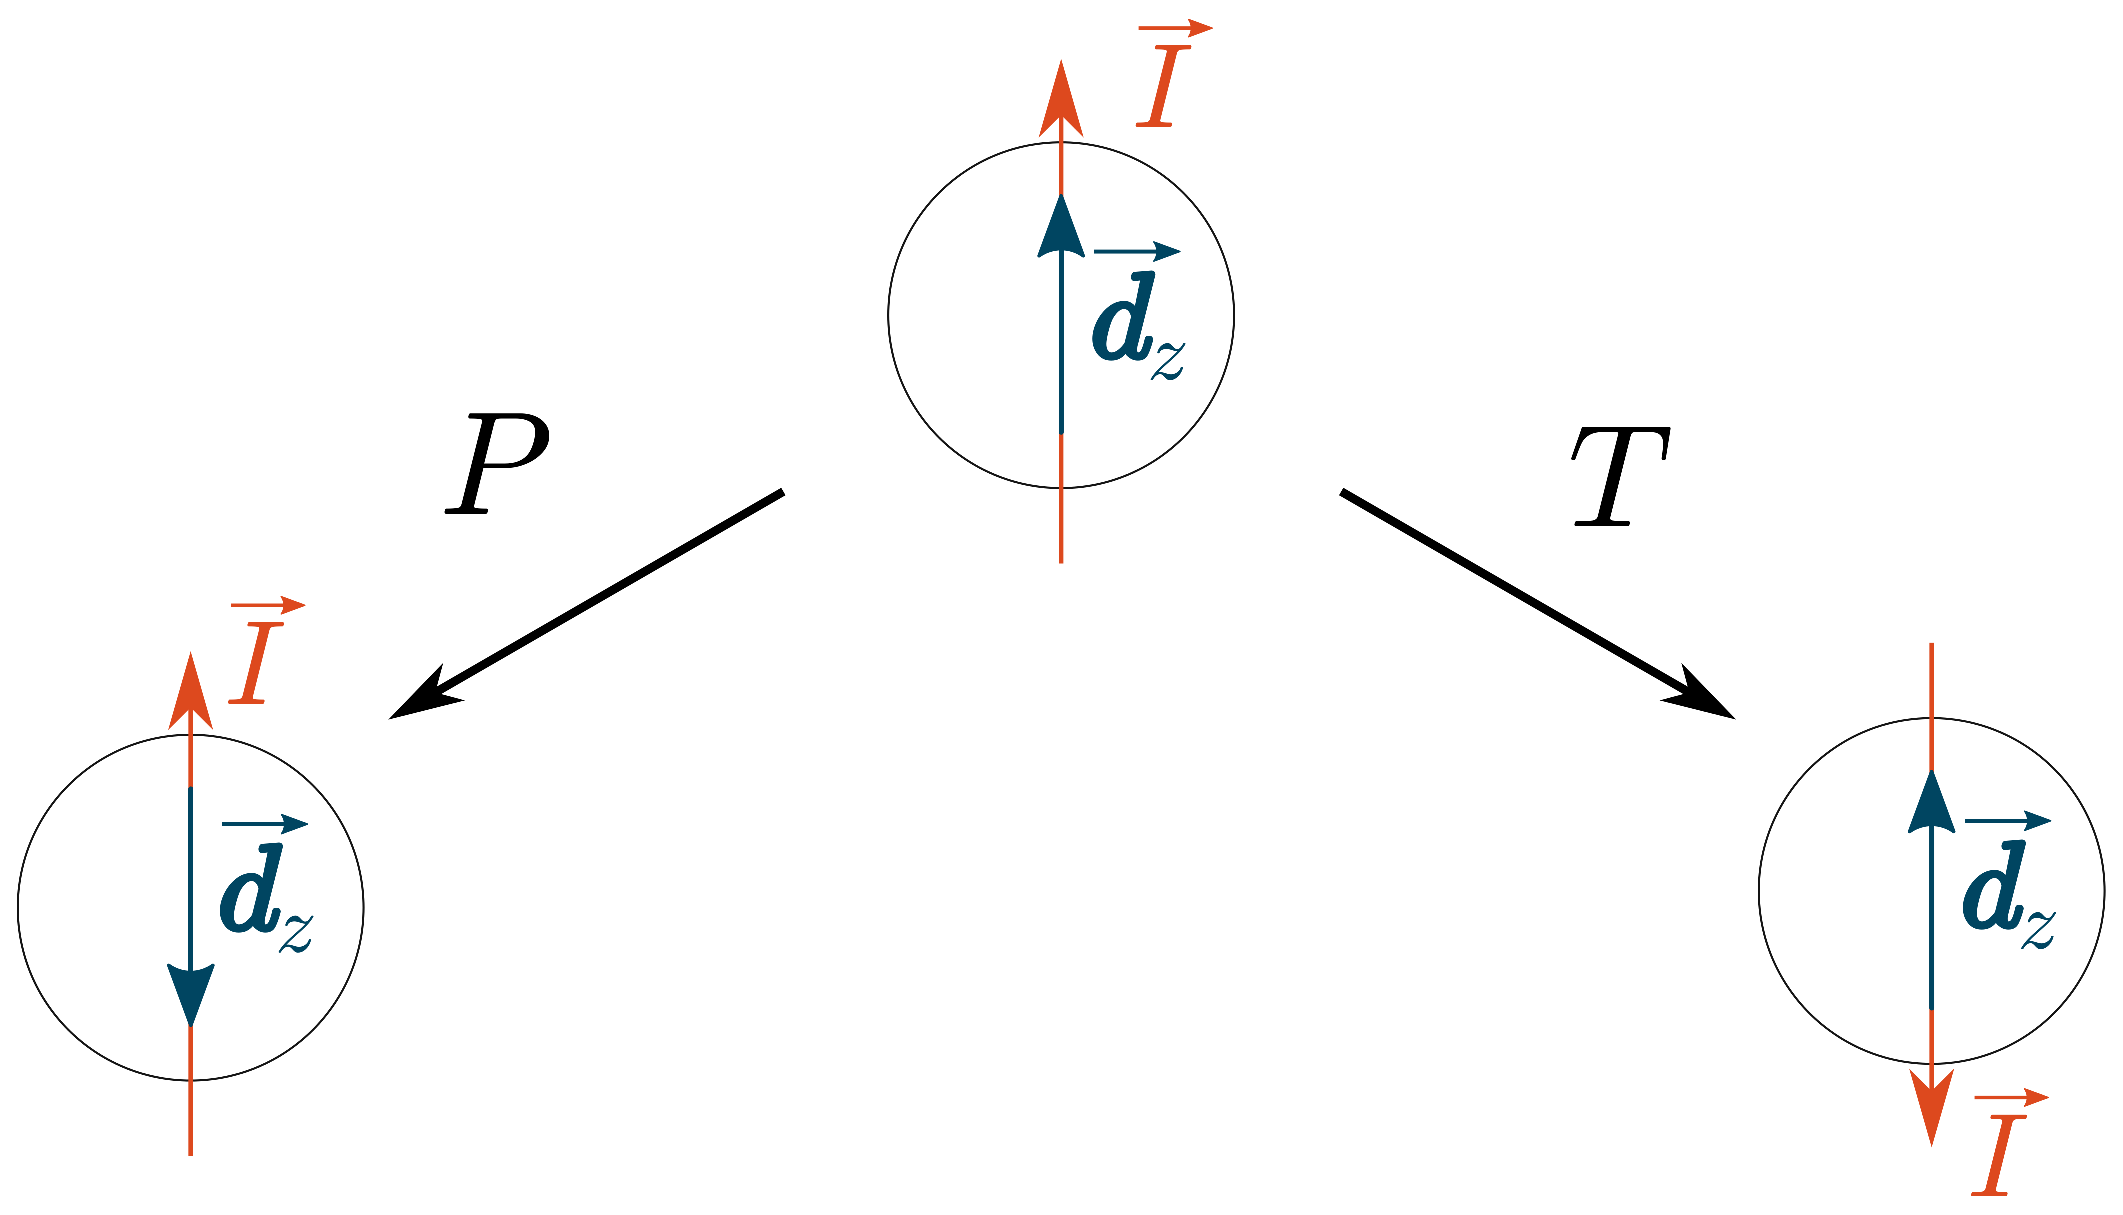
\includegraphics[scale=0.3]{./figures/EDM.eps}
\caption{\label{fig:ParityTimeEDM} This diagram show the $P$ and $T$ transforms of a particle with angular momentum $I$ and a finite EDM $\textbf{d}$. The spatial EDM defined in  is $P$-odd and $T$-even. However as the EDM must be in the direction of the angular momentum of the particle which is $P$-even and $T$-odd there is a contradiction and the EDM violates $P$ and $T$.}
\end{figure}
Experiments aimed at measuring these permanent EM moments present a promising avenue for possibly detect or at least constraining 
\section{Lorentz symmetry violation} \label{sec:Lorentz}
Tests of Lorentz violation also span both high-energy, cosmological scales down to low energy precision tests. $\gamma$ ray bursts are a potential test of quantum gravity  \cite{Amelino1998}. A superluminal charged particle will rapidly radiate photons until it no longer exceeds the speed of light \cite{Coleman1997}. A review on potential high energy Lorentz violating tests can be found in Ref. \cite{Coleman1999}. 

Like the discrete symmetries, Lorentz symmetry is one of the most fundamental symmetries in nature. It forms the basis of modern physics as the cornerstone to special relativity. Local Lorentz invariance (LLI) states that there is no preferred reference frame of the universe and the laws of physics are unchanged when the orientation of the system (rotation) or speed of the system (boosts) is changed. Due to its importance, considerable effort has been made over the last century to test and quantify its validity through experiments \cite{Michelson1887, Kennedy1932, Ives1938, Robertson1949, LorentzTestSeries}.  \\
\linebreak
In the current SM Lorentz invariance, along with combined CPT, is always conserved. However, there are many proposals for new physics BSM such as GUT and String theories that require LLI to be violated \cite{Kostelecky1989,  Damour, Gambini1999, Pospelov2012, Kostelecky1995, Mavromatos2007, Liberati2013}.  Like the discrete symmetries above, LLI is suspected to be a low-energy effective property which is spontaneously broken at higher energies due to an underlying theory. Unlike violation of the discrete symmetries however,  there  are no sources of LLIV in the SM and any measurement of some anisotropy will be the result of some unknown greater underlying theory. Therefore an extension to the SM in Refs. \cite{Colladay1997, Colladay1998, Kostelecky1999, LorentzDataTables2017} has been proposed which contains LLIV terms in the SM Lagrangian while preserving other desirable properties of the SM such as renormalizability and gauge invariance. This extension to the SM provides a framework to represent and quantify particular LLIV mechanisms in experiments. \\
\linebreak
The possiblility of these new physics has led to a renewed concerted effort in detecting LLIV using modern experimental methods using more sophisticated techniques. These include  resonance cavity experiments \cite{Muller2005, Muller2003, Wolf2004}, Doppler shift experiments \cite{Lane2005, Saathoff2003} and clock comparison experiments \cite{Prestage1985, Chupp1989, Hohensee2013, Dzuba2016}. These experiments rely on measuring slight variations in results when the orientation or speed of the system is changed and therefore require extremely precise measurements. Currently, these experiments have only resulted in null measurements, however they have constrained the LLIV parameters in the SM extension extensively. A yearly review on the current status of LLIV can be found in \cite{LorentzDataTables2019} which provides an exhaustive list of the constraints on LLIV parameters in the SM extension.



\section{Violation in nuclear, atomic and molecular systems}
As mentioned previously, while violation of the LLI and $CP-$ symmetries are spontaneously broken at extremely high energies, signatures of these violations may manifest at low energies. The realm of atomic and nuclear physics is a perfect domain to search for these signatures as they offer high sensitivity at relatively low cost. The concept of using atomic interactions to detect LLIV has long been considered \cite{Hughes1960, Drever1961, Prestage1985, Lamoreaux1986, Lamoreaux1989}


Atoms provide an optimal space to test the Standard Model as all SM interactions are found in atomic theory and can be probed.


$CP$- violating permanent electrodynamic moments are expected to be observed in composite particles and systems  such as atoms, nuclei and baryons and interpreted as parameters of $CP$- violating interactions in the lepton and quark-gluon sectors. In this paper we focus on the magnetic quadrupole moment (MQM) of the nucleus in particular, which is the lowest order magnetic moment that is forbidden in quantum systems by the time reversal invariance ($T$) and  parity ($P$).  For an in-depth review on symmetry violating electromagnetic moments including the MQM see Ref. \cite{GF2004, KhriplovichPNC, SFK1984, Roberts2015, KhriplovichCP, Pospelov2005}. The MQM of composite systems such as the deuteron \cite{Liu2012} have previously been investigated. The search for MQM in comparison with the electrostatic $T,P$-violating moments (EDM, Schiff and octupole moments) may have the following advantages:

\begin{itemize}
\item The nuclear EDM  in neutral atoms and molecules are completely screened \cite{Schiff1963}. The Schiff and octupole moments have an additional second power of a very small nuclear radius. The magnetic interaction is not screened. The MQM contribution to atomic EDM typically is an order of magnitude larger than the contribution of the Schiff moment and several orders of magnitude larger than the octupole contribution \cite{SFK1984, Flambaum1997}.  

\item In quadrupole deformed nuclei MQM is enhanced by an order of magnitude \cite{Flambaum1994}, therefore, the MQM contribution to atomic EDM may be two orders of magnitude larger than the Schiff moment contribution.

\item In the expression for the Schiff moment there is a partial cancellation between the first term and the second (screening) term. There is also a screening correction to the octupole moment \cite{ Flambaum1986, SFK1984, Flambaum2012}.

\item In the Hg and Xe atoms  where the most accurate measurements of atomic EDM have been performed, the valence nucleon is a neutron. Therefore, the electrostatic moments (EDM, Schiff and octupole) moments do not appear directly, they exist due to the nuclear polarization effects \cite{Flambaum1986}. Due to the screening effect and the indirect polarization origin of the Schiff moment the nuclear calculations are rather unstable.
In the case of the MQM moment both valence protons and neutrons  contribute directly, and the result is expected to be more accurate\cite{Flambaum2014}.  

\end{itemize}

 A promising method of measuring $CP$- violating moments is in diatomic molecular experiments where the effective electric field is significantly larger than those directly accessible in laboratory experiments.  There is a considerable body of work for calculating the effective electric field in diatomic molecular systems which may be experimentally viable. Both theoretical and experimental progress has been made in measuring the $T,P-$ odd effects in  YbF\cite{Hudson2011, Mosyagin1998, Quiney1998, Parpia1998, Kozlov1994, Nayak2009, Steimle2007, Abe2014}, HfF$^+$ \cite{Cossel2012, Loh2013, Petrov2007, Fleig2013, Meyer2006, Skripnikov2008Hf, Le2013, Skripnikov2017Hf, Cairncross2017}, ThO \cite{Petrov2014, Meyer2008, Skripnikov2013ThO, Skripnikov2014ThO, Titov2015ThO, Fleig2014, Denis2016, Baron2017}, ThF$^+$\cite{Loh2013, Skripnikov2015Th, Denis2015}, TaN \cite{Skripnikov2015Ta, Fleig2016TaN} and TaO$^+$ \cite{Fleig2018} particularly in relation to the nuclear Schiff moment and electron EDM.   In section \ref{sec:MQMmolecule} we present the molecular energy shift due to the nuclear MQM for these molecules.
 
 
 The PNC effects appear due to mixing of opposite parity states in atoms and molecules by the weak interaction between the nucleus and electrons. The field  of PNC in atoms and molecules has been thoroughly reviewed in Refs.  \cite{KhriplovichPNC,GingesReview,RobertsReview}. It was noted in Ref.  \cite{FS78} that the nuclear quadrupole moment induces a tensor PNC weak interaction between the nucleus and electrons (see also  \cite{KhriplovichPNC,KP91}). In Ref. \cite{Flambaum2016} it was argued that these tensor  effects of the weak quadrupole moments are strongly enhanced for deformed nuclei and may get a significant additional enhancement due to mixing of  close atomic and molecular levels of opposite parity with a  difference of the electron angular momenta $|J_1-J_2| \le 2$. These selection rules are similar to that for the effects of the time reversal ($T$) and parity ($P$) violating nuclear magnetic quadrupole moment (MQM). Therefore, nuclei, molecules and molecular levels  suggested for the MQM search in Ref. \cite{Flambaum2014},  for example,  $|\Omega |=1$ doublets in the molecules $^{177}$HfF+, $^{229}$ThO, $^{181}$TaN will also have enhanced effects of the weak quadrupole (see section \ref{sec:PNC}). Following our proposal, there has been recent experimental interest in using the weak quadrupole moment to study PNC effects in HfF$^{+}$ molecules (used to measure electron electric dipole moment \cite{Cairncross2017}) and parity violation in $^{173}$Yb \cite{Antypas2017} and $^{163}$Dy \cite{Leefer2017} atoms. 
 
Violation of LLIV in nuclear systems using the tensor interaction does not require study of nuclear transitions like other LLIV parameters as the angular momentum projections are different. The $C_0^{(2)} = c_{xx} + c_{yy} - 2c_{zz}$ is the LLIV tensor interaction in the laboratory frame where the quantization axis (same as the deformation axis deformed nuclei, see next chapter) lies along the $z$ axis.
\chapter{Properties of deformed nuclei}
The existence of non-spherical nuclei has been suspected since the 1930s where anomalous behaviour was observed in the hyperfine structure in isotopes of Eu ($Z=63$) and Lu ($Z=71$) by H. Schuler and Th. Schmidt \cite{Schuler1935(1), Schuler1935(2)}. Soon after this discovery, H. B. G. Casimir published an explanation of these results and posited the anomaly could be explained by the existence of an permanent electric quadrupole moment of the nucleus which interacts with the atomic electrons \cite{Casimir1935, Casimir1936}. The origin of this nuclear quadrupole moment was orginally ascribed to the existence of an unpaired valence proton with nuclear spin $I_t$ which induces and electric quadrupole moment  $Q_{p,\text{val}}$ of the nucleus by the equation \cite{BohrMottVol1},
\begin{align}\label{eq:valQ}
Q_{p,\text{val}} &=  - \dfrac{I_t-1/2}{I_t + 1}0.009A^{2/3} \ \text{barn}.
\end{align}  
This single particle description is incomplete for several reasons. Firstly, it does not account for the quadrupole moments of nuclei with unpaired neutrons which also have significant quadrupole moments, for example $^{163}_{66}$Dy has an unpaired neutron with an experimental quadrupole moment $Q_p = +2.318(2) \ \text{barn}$ \cite{Stone2005}. Secondly, the magnitude of a quadrupole moment from a single proton is significantly less than those observed in experiment. For example consider $^{181}_{73}$Ta, which has total nuclear spin $I_t=7/2^{+}$, using eqn (\ref{eq:ValQ}) results in a quadrupole moment of $Q_{p,\text{val}} = -0.192 \ \text{barn}$. This is significant less (along with opposite sign) than the experimental $Q_p = +3.17(2) \ \text{barn}$. Therefore the quadrupole moment of a nucleus must be a collective effect of the nucleus involving a large amount of the nuclear matter and cannot be accounted for by a single nucleon. 
\begin{figure}
\centering
\begin{subfigure}[b]{0.48\textwidth}
\centering
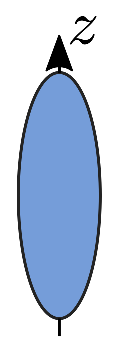
\includegraphics{./figures/prolate.eps}
\caption{Prolate deformation of a nucleus. Here the $z$ axis is the symmetry axis.}
\end{subfigure}	
\quad
\begin{subfigure}[b]{0.48\textwidth}
\centering
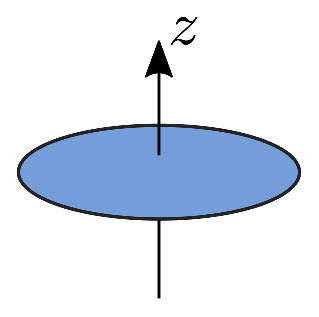
\includegraphics{./figures/oblate.eps}
\caption{Oblate deformation of a nucleus. Here the $z$ axis is the symmetry axis.}
\end{subfigure}
\end{figure}
\section{The Nilsson Model}
While collective effects of the nucleus have been considered for a significantly long time with the liquid drop model, they were not considered in the context of the microscopic prospect of the nucleus. The isometric shell model is an independent single particle model where the nucleons are modeled in a mean field approximated by the interaction of the other nucleons which was very successful in predicting the closed shells in spherical nuclei\cite{Mayer1949, Jensen1949}. While the spherical shell model was successful in predicting closed shell of spherical nuclei, it had limitations when considering highly deformed nuclei. Collective properties of the nucleus include large quadrupole moments and nuclear fission. Non-spherical nuclei were first explored in depth by Rainwater in 1950 \cite{Rainwater1950}. A single-particle model which accounts for the asymmetry of the nucleus was developed by S. G. Nilsson in 1955 \cite{Nilsson1955}. This model, known as the Nilsson model, uses an anisiotropic harmonic oscillator potential to describe the nuclear potential the nucleons move in. The complete Hamiltonian of the Nilsson model is given by \cite{Nilsson1955, Gustafson1967},
\begin{align} \label{eq:NilssonHamiltonian}
H = \dfrac{\textbf{p}^2}{2m} + \dfrac{1}{2}m \left[\omega_x\left(\textbf{x}^2 + \textbf{y}^2\right) + \omega_z \textbf{z}^2\right] + C\textbf{l}\cdot \textbf{s} + D \left(\textbf{l}^2 - \left<I^2\right>\right)
\end{align}
Both the spin-orbit term ($\textbf{l}\cdot \textbf{s}$) and the  $\textbf{l}^2 - \left<I^2\right>$ terms were included to reproduce the magic numbers in the spherical limit.   Considering quadrupole deformations only, the energies on the perpendicular are equal $\omega_x = \omega_y = \omega_{\perp}$. In the regions of closed major shells the equilbrium shape of the nucleus is spherical \cite{Nilsson1955}. The only oblate candidates are those where the protons or neutrons  are near the end of a major shell ($N$). Therefore the vast majority of nuclei are prolate deformed, however the Nilsson model is also applicable for oblate nuclei.
\begin{align*}
\omega_{\perp^{2}} = \omega_0^2\left(1 + \dfrac{2}{3}\delta\right) \\
\omega_z^2 = \omega_0^2\left(1 - \dfrac{4}{3}\delta\right)
\end{align*}
  In the spherical shell model the orbit with angular momentum $I$ has degeneracy $2I + 1$ nucleons. This degeneracy is broken in the Nilsson model for deformed nuclei where the projection of the angular momentum onto the symmetry axis, $\Omega$, is the good quantum number (see Figure \ref{fig:prolate_AM}). Each of these $\Omega$ states are doubly degenerate. The consequences of a deformed nucleus on the quantum states of the constituent nucleons can be deduced from two simple physical arguments. Consider the non-rotating, intrinsic (body) frame of the nucleus. Where $\Omega$ is the projection of the nucleons angular momentum $I$ on the deformation axis. 
\begin{figure}
\centering
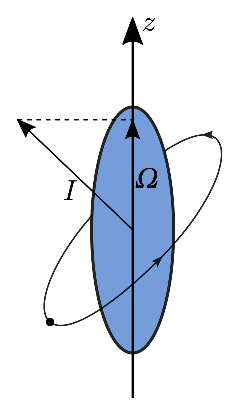
\includegraphics[scale=1]{./figures/prolate_AM.eps}
\caption{Projection of angular momentum of a prolate deformed nucleus onto the symmetry axis in the intrinsic frame. Here $I$ is the angular momentum of the nucleon and $\Omega$ is its projection on the axis of deformation.}
\label{fig:prolate_AM}
\end{figure}
By definition the projection of total angular momentum on the symmetry axis $\Omega$ is the sum of the projection of the orbital angular momentum, $\Lambda$ and the projection of the spin angular moment$\Sigma = \pm 1/2$.  $\Omega = \pm\tfrac{1}{2}, \pm\tfrac{3}{2},  \pm\tfrac{5}{2},  ... ,  \pm\tfrac{I}{2}$

%\begin{align*}
%\delta \approx 0.95 \beta
%\end{align*}
The deformation of the nucelar field implies important modifications of the nucleonic motion. Each orbit may be occupied twice, corresponding to the two possible signs of $\Omega$. The absence of degeneracuies implies a very simply coupling scheme for the particle motion. Thus, in an odd-A nucleus the ground-state spin is equal to the value of $\Omega$ for the orbit occupied by the last nucleon except for $\Omega=1/2$ \cite{Nilsson1955}. 


To classify each constituent nucleon in the deformed nucleus we use the Nilsson model of deformed nuclei \cite{Nilsson1955, BohrMottVol2}. The independent particle model will only describe how a single nucleon will behave in the mean field/potential. In the case of an atom this is a relatively simple and stable approach. This is because in an atom, to a first approximation, the electrons experience a potential from the much larger point like nucleus. It is only in lower approximations that you take into account the inter electron potential by using methods such as Hartree Fock. However in the nucleus there is no centre source of potential, it all comes from the inter-nucleon interactions which is not completely understood. Therefore any mean field potential ascribed to the nucleus is going to be inherently unstable, especially when considering larger nuclei. This results in a anisotropy of the nucleus which has interesting properties when trying to understand nuclear physics.

In this paper we will use the empirically successful Nilsson model \cite{Nilsson1955, BohrMottVol2} (deformed oscillator model)  to describe the single particle model states of the constituent nucleons in deformed nuclei and calculate the magnitude of the quadrupole and momentum tensors. The Nilsson Hamiltonian which governs the system is,

which has the form of an asymmetric 3D oscillator model where we have chosen the $z-$axis as the axis of deformation. Here $m$ is the nucleon mass, $\omega_z$ and $\omega_{\perp}$ are the nucleon oscillation frequencies along the $z-$axis and the perpendicular  plane respectively.  The deformation of the nucleus has the effect of splitting the degeneracy of the nuclear energy levels within the oscillator shell. The greater the deformation the greater the splitting. Each nucleon can be characterised by the set of quantum numbers $\left[N n_z \Lambda \pm\Omega\right]$ \cite{BohrMottVol2}  where $N = n_z + n_x + n_y$ and each $n_i$ ($i = x, y, z$) is the principal quantum number in the direction of $i$, $\Lambda$ and $\Omega$ are the nucleon's orbital and total angular momentum projection on the deformation axis respectivly. Each energy level is doubly degenerate for $\pm\Omega$. The average oscillator frequency   is given by $\hbar\bar{\omega} = \hbar/3\left(2\omega_{\perp} + \omega_z\right) \approx 45A^{-1/3} - 25A^{-2/3} \ \text{MeV}$\cite{Brown2016}. Second order tensor properties  in deformed nuclei exhibit a collective enhancement compared to vector properties. We indirectly include spin-orbit and angular momentum terms of the Nilsson Hamiltonian through the split level Nilsson energy plots in ref. \cite{BohrMottVol2}.

Consider the magnetic dipole moment  which is proportional to  the projection of the total angular momentum $\Omega$ to the nuclear axis. In an even-even nucleus all the nucleons are paired and therefore the magnetic dipole moment of the $+\Omega$ state cancels with the $-\Omega$ state resulting in no net magnetic dipole moment of the nucleus. For an odd $A$ nucleus  the magnetic dipole moment of the entire nucleus is simply the dipole moment of the odd nucleon. This is the well known Schmidt model of the nucleus. The cases for second order tensor properties of the nucleus are different. For  nucleons in the  $+\Omega$ and the $-\Omega$ states tensor properties  are additive. Therefore there is a collective effect and many nucleons contribute to the tensor properties of the nucleus.

In the Nilsson model we consider the nucleus in the intrinsic frame which rotates with the nucleus. However the nucleus itself rotates with respect to the fixed laboratory frame \cite{BohrMottVol2}. Due to this rotation the tensor properties transform between the intrinsic  and laboratory frame. The relationship between these two frames is \cite{BohrMottVol2}
\begin{align} \label{eq:RotationalFactor}
A^{Lab} = \dfrac{I\left(2I - 1\right)}{\left(I + 1 \right)\left(2I + 3\right)}A^{Intrinsic},
\end{align}
where $I=I_z= \left|\Omega\right|$ is the projection of total nuclear angular momentum (nuclear spin) on the symmetry axis. This expression shows that only in nuclei with spin $I > 1/2$ can we detect these second order tensor properties. 
The collective enhancement of MQM for some  heavy deformed nuclei were estimated in \cite{Flambaum1994, Flambaum2014} where they considered the contribution using a spherical wave function basis. In this work we will use the Nilsson model of the the nucleus  which is an empirically successful single particle model which accounts for the quadrupole deformation of a nucleus by using an anisotropic oscillator potential \cite{Nilsson1955, Mottelson1955, BohrMottVol2}. In the Nilsson model the deformation breaks the degeneracy of the isotropic shell model which results in several overlapping partially filled nuclear shells containing a large number of nucleons.  Each nucleon in the Nilsson model is defined in the Nilsson basis $\left[Nn_z\Lambda\Omega\right]$ where $N$ is the principle shell number ($N = n_x + n_y + n_z$), $\Lambda$ is the projection of the orbital angular momentum on the deformation axis (chosen to be the $z$-axis) and $\Omega = \Lambda + \Sigma$ is the projection of the total angular momentum of the nucleon on the deformation axis.


To illustrate why the MQM tensor should be enhanced in quadrupole deformed nuclei let us compare it with  the EDM vector property of nuclei. The direction of the EDM of a nucleon is characterised by its angular momentum projection on the deformed nucleus axis $\Omega$. In the case of the vector properties such as EDM and magnetic moment the contributions of $\Omega$ and $-\Omega$ cancel each other and  there is no enhancement in the quadrupole deformed nuclei. For the second rank tensors such as MQM and nuclear electric quadrupole moment the contributions of $\Omega$ and $-\Omega$ double the effect. There are many nucleons in the open shells of deformed nuclei and this leads to a collective enhancement of second rank tensor properties.
\section{The distribution of neutrons in the nucleus}
Measuring the NQMN, $Q_{n}$,  is a very difficult  task as neutrons are electrically neutral particles unlike the electric quadrupole moment of the nucleus which was first observed and measured nearly a century ago by H. Schuler and Th. Schmidt \cite{Schuler1935(1), Schuler1935(2), Casimir1935} by studying the hyperfine structure of rare earth elements. The NQMN is an important property which will give insight not only into the structure of  atomic nuclei but also other dense collections of neutrons such as neutron stars \cite{Brown2000, Furnstahl2002, Typel2001, Reinhard2010} and also the theory of atomic parity nonconservation. For the last two decades there has been increasing interest in understanding the distribution of neutrons compared to protons in atomic nuclei known as the neutron skin. This focus has largely been on the spherical distribution of neutrons (measurement of the root mean square radius of neutrons) and there has been a large amount of experimental effort in measuring the spherical distribution \cite{Clark2003, Trzcinska2001, Lenske2009, Abrahamyan2012}. 


Rewriting equations (\ref{eq:CollectiveMDim}), (\ref{eq:CollectiveQDim})  and, the relation between the longitudinal  and perpendicular frequencies in dimentionless quantities $\eta = \bar{\omega}/\omega_z$ and $\xi = \bar{\omega}/\omega_{\perp}$ we have the equations,
\begin{align}
3 &= \dfrac{1}{\eta} + \dfrac{2}{\xi} \label{eq:average} 
\end{align}

The nucleon angular momentum dependence shows up in the order of the split energy branches in the Nilsson plots \cite{Nilsson1955, BohrMottVol2}.
%It should be noted that there is no explicit dependence on the angular momentum of the nucleons. This is because the angular momentum dependence is in the order of the nucleons in the Nilsson plots used to find the nucleonic configuration. 
The parameters $\eta$ and $\xi$ can be viewed as deformation parameters of the nuclei. For positive deformation $\eta > 1$ (prolate) and for negative deformation $\eta < 1$ (oblate). As there is a predominance on nuclear prolate deformations in nature most of the nuclei we consider will be prolate. \\


\chapter{The weak quadrupole moment and Lorentz violation in nuclei}
\textit{The results of this chapter have been published in reference \cite{LFWQM2018} } \\
Int his chapter I present the calculations of the local Lorentz invariance violating (LLIV) parameters $C_{2}^{(0)}$ and the weak quadrupole moments (WQM) of deformed nuclei. \\   
\linebreak
Non-spherical nuclei present a lucrative avenue for studying the existence and magnitude of second order tensor properties due to the collective properties of deformed nuclei. In this chapter we focus on the quadrupole moment of the nonspherical  distribution of neutrons in the nucleus, $Q_{n}$,  the weak quadrupole moment (WQM), $Q_{W}^{(2)}$,  and the violation of Local Lorentz invariance (LLI) in the nucleon sector. \\
\linebreak





 However, the best current laboratory limits are from clock comparison experiments \cite{Prestage1985, Chupp1989, Hohensee2013, Dzuba2016} in particular the tensor LLIV parameters $c_{ij}$ for the neutron in \cite{Smiciklas2011} using a $^{21}$Ne clock and for the proton in \cite{Wolf2006} using $^{133}$Cs clocks which was further constrained by 4 orders of magnitude in \cite{Flambaum2016}.  In Ref. \cite{Brown2016} the $s-d$ shell model calculations of the tensor LLIV effects have been performed in $^{21}$Ne, $^{131}$Xe and $^{201}$Hg nuclei. It was demonstrated that virtual excitations from the nuclear core enhance the nuclear quadrupole moment and suppress the LLIV tensor.  The results of the $s-d$ shell model calculations have been supported by the calculations in the Hartree-Fock-Bogoliubov model published in the same paper \cite{Brown2016}.

The best laboratory limits on the Michelson-Morley type LLIV tensor in the photon sector has been obtained in Ref. \cite{FlambaumRomalis2017}  using the $^{21}$Ne clock data from  \cite{Smiciklas2011}.  
The limits on the LLIV parameters  obtained using astrophysical measurements and laboratory experiments can be found in \cite{Kostelecky1999, LorentzDataTables2017}. In the present paper we study  the LLIV momentum tensor Hamiltonian $\delta H$  \cite{Kostelecky1999}
\begin{align} \label{eq:HamilQuadShift}
\delta H = \left[-c_{ij} -\dfrac{1}{2}c_{00}\delta_{ij}\right]\dfrac{p_ip_j}{m^2},
\end{align}
 where $m$ is the nucleon mass,  to describe the tensor parameter $c_{ij}$  for the LLIV interaction \cite{Kostelecky1999} in the laboratory frame. 
\section{Quadrupole moment of neutron distribution in deformed nuclei}

The quadrupole moment tensor along the symmetry axis of the nucleus in cartesian coordinates is given by
\begin{align}\label{eq:QMomentStandard}
Q_{zz} = Q = 2\left<z^2\right> - \left<x^2\right> - \left<y^2\right> .
\end{align}
From the virial theorem for bound particle in a harmonic oscillator potential the average kinetic energy $\left<T\right>$ and average potential energy $\left<U\right>$ are equal. Using the well known energy spectrum for the harmonic oscillator $E_{n} = \hbar\omega(n + 1/2)$  the average of the square of the position in the $z$ direction is,
\begin{align}\label{eq:zExpectation}
m\omega_z^2\left<z^2\right>&= \hbar\omega_z\left(n_z + 1/2\right) 
\end{align}
  with similar relations for $\left<x^2\right>$ and $\left<y^2\right>$. Using equations (\ref{eq:QMomentStandard}), (\ref{eq:zExpectation}) and $n_x + n_y = N - n_z$ the contribution to the quadrupole moment from a single nucleon in the quantum state $\left[N n_z \Lambda \Omega\right]$ is given by
\begin{align} \label{eq:QMomentNucleon}
q_{i,\nu} &= \dfrac{\hbar}{m}\left[\dfrac{\left(2n_z + 1\right)_{i,\nu}}{\omega_z} - \dfrac{\left(N -n_z + 1\right)_{i,\nu}}{\omega_{\perp}}\right] ,
\end{align}
where $\nu = p,n$ for the $i$th proton or neutron respectively. The total quadrupole moment is the sum of all the respective nucleon quadrupole moment contributions
\begin{align}
Q_{\nu} &= \sum_{i} q_{i,\nu} \nonumber\\
&= \dfrac{\hbar}{m}\left[\dfrac{1}{\omega_z}\sum_{i}\left(2n_z + 1\right)_{i,\nu} - \dfrac{1}{\omega_{\perp}}\sum_{i}\left(N -n_z + 1\right)_{i,\nu}\right]. \label{eq:CollectiveMDim} 
\end{align}
\section{Lorentz invariance violation  in deformed nuclei}
Taking the expectation value of equation (\ref{eq:HamilQuadShift}), we find that the LLIV energy shift  for a nucleus with $N_{\nu}$ nucleons with angular momentum projection $I_{\nu}$ is given by 
%\cite{Kostelecky1999},
\begin{align} \label{eq:MomentumEnergyShift}
<\delta H>_{\nu} = \dfrac{1}{6m}C_{0, \nu}^{(2)}\sum_{N=1}^{N_{\nu}}\left<I_{\nu},I_{\nu}\left|\hat{M}\right|I_{\nu},I_{\nu}\right> 
\end{align}
where the $\hat{M} = 2\hat{p}_z^2 - \hat{p}_x^2 - \hat{p}_y^2$ is the momentum tensor operator for $p_ip_j$ in the SME in cartesian coordinates. We use the standard notion $C_{0, \nu}^{(2)} = c_{xx} + c_{yy} -2c_{zz}$ \cite{Kostelecky1999}. We define the single nucleon LLIV momentum tensor as,
\begin{align} \label{eq:LLIVMomentum}
\bar{m}_{i, \nu} =  \left<I,I\left|2\hat{p}_z^2 - \hat{p}_x^2 - \hat{p}_y^2\right|I,I\right>.
\end{align}
Using the virial theorem for a harmonic oscillator ($\left<T\right>=\left<U\right>$) and energy spectrum again we have the average square of the momentum given by
\begin{align} 
\dfrac{\left<p_z^2\right>}{2m} &= \dfrac{\hbar\omega_z\left(n_z + 1/2\right)}{2} \label{eq:pExpectation}
\end{align}
with similar expressions for $x$ and $y$ coordinates. \\
\linebreak
Using equations (\ref{eq:LLIVMomentum}) and (\ref{eq:pExpectation}) we write the contribution to the LLIV tensor of a nucleon as,
\begin{align} \label{eq:MDimensionful}
\bar{m}_{i,\nu} &= \hbar m\left[\left(2n_z + 1\right)_{i,\nu}\omega_z - \left(N - n_z + 1\right)_{i,\nu}\omega_{\perp}\right].
\end{align}
The total LLIV tensor, $M_{\nu}$,  for the nucleus is the sum of all respective nucleons
\begin{align}
M_{\nu} &= \sum_{i,\nu} \bar{m}_{i,\nu} \nonumber \\
&= \hbar m\left[\omega_z\sum_{i}\left(2n_z + 1\right)_{i,\nu} - \omega_{\perp}\sum_{i}\left(N - n_z + 1\right)_{i,\nu}\right]. \label{eq:CollectiveQDim}
\end{align}
This will result in a quadrupole energy shift given by
\begin{align} \label{eq:LLIVEnergyShift}
\left<\delta H\right>_{\nu} = \dfrac{M_{\nu}}{6m} C_{0,\nu}^{(2)}.
\end{align}

\begin{align}
Q_{\nu} = \dfrac{41.5\text{ MeV}\text{fm}^2}{\hbar\bar{\omega}}\left[\eta\sum_{i}\left(2n_z + 1\right)_{i,\nu}  - \xi\sum_{i}\left(N - n_z + 1\right)_{i,\nu}\right]&
\label{eq:QDimensionless}
\end{align}
\begin{align}
M_{\nu} = \hbar\bar{\omega}m\left[\dfrac{1}{\eta}\sum_{i}\left(2n_z + 1\right)_{i,\nu} - \dfrac{1}{\xi}\sum_{i}\left(N - n_z + 1\right)_{i,\nu}\right]. & \label{eq:MDimensionless}
\end{align}
\section{Example calculation of $Q_{\nu}$ and $M_{\nu}$ for the $^{173}$Yb nucleus}
To illustrate the process of calculating NQMN and LLIV values we will present the calculation of $^{173}$Yb as an example. To begin we find the nuclear configuration of protons and neutrons in the deformed field using the energy level plots presented in \cite{Nilsson1955,BohrMottVol2} by filling each non-degenerate $\Omega$ energy branch with two nucleons until all the nucleons have been distributed. To find the correct deformation, $\delta$, from which to fill we use the experimental value of the nuclear spin (which is solely due to the unpaired nucleon). The filling must be done such that the unpaired nucleon is in the correct spin state. The nuclear spin of $^{173}$Yb is $5/2^{-}$ due to an unpaired neutron. Using the method described above we find that this is possible with a minimum deformation of $\delta \approx 0.3$. Here we will only present the configuration of the partially filled $N$ shells. The numbers for each full shell is given in Table \ref{table:FullShellNz}. The incomplete neutron and proton shells in $^{173}$Yb are $N = 5,6$ and $N = 4,5$ respectively. The nucleon configuration of the incomplete shells are given in Table \ref{table:YbConfig}.
\begin{landscape}
\begin{table*} 
\centering
\caption{Nilsson configuration of $^{173}$Yb nucleons: This table shows the nuclear configuration of nucleons in the Nilsson model for $^{173}$Yb generated from the Nilsson plots in Ref. \cite{BohrMottVol2}. This table shows only partially filled $N$ shells. All preceding shells are completely filled. \label{table:YbConfig}}
\begin{tabular}{p{1.5cm}lcc@{\hspace{1cm}}p{1.5cm}lcc}
\toprule
\toprule
\multicolumn{2}{c}{\parbox[c][][c]{2cm}{\vspace{3pt}Neutrons in incomplete shells\vspace{3pt}}} & $\sum \left(2n_z + 1\right)_n$ & $\sum \left(N - n_z + 1\right)_n$ & \multicolumn{2}{c}{\parbox[c][][c]{2cm}{\vspace{3pt}Protons in incomplete shells\vspace{3pt}}} & $\sum \left(2n_z + 1\right)_p$ & $\sum \left(N - n_z + 1\right)_p$\\ 
\midrule
 $2f_{7/2}$: &\parbox[c][][l]{2cm}{\begin{flushleft}
 $\pm 1/2[530]$, $\pm 3/2[521]$, $ \pm 5/2[512]$\end{flushleft} }&  30 & 24 & $1g_{7/2}$: & \parbox[c][][c]{2cm}{\begin{flushleft}
$\pm 1/2[431]$, $\pm 3/2[422]$, $ \pm 5/2[413]$
\end{flushleft} }& 30 & 18 \\
 $1h_{9/2}$: &  \parbox[c][][c]{2cm}{\begin{flushleft}
 $\pm 1/2[541]$, $\pm 3/2[532]$, $ 5/2[523]$\end{flushleft} } & 37 & 14 & $2d_{5/2}$: & \parbox[c][][c]{2cm}{\begin{flushleft}
 $\pm 1/2[420]$, $\pm 3/2[411]$ \end{flushleft} } & 16 & 14 \\
 $3p_{3/2}$: & \parbox[c][][l]{2cm}{\begin{flushleft}
$\pm 1/2[521]$\end{flushleft}} & 10 & 8 & $2d_{3/2}$: & \parbox[c][][c]{2cm}{ \begin{flushleft}
$\pm 1/2[521]$ \end{flushleft} } & 6 & 8 \\
 $1h_{11/2}$: & \parbox[c][][c]{2cm}{\begin{flushleft}
 $\pm 1/2[550]$, $\pm 3/2[541]$, $\pm 5/2[532]$, $\pm 7/2[523]$, $\pm 9/2[514]$, $\pm 11/2 [505]$\end{flushleft}}   & 72 & 42 & $1g_{9/2}$: &  \parbox[c][][c]{2cm}{\begin{flushleft}
$\pm 1/2[440]$, $\pm 3/2[431]$, $ \pm 5/2[422]$, $\pm 7/2[413]$, $\pm 9/2[404]$ \end{flushleft} }  & 50 & 30 \\
 $1i_{13/2}$: & \parbox[c][][l]{2cm}{\begin{flushleft}
 $\pm 1/2[660]$, $\pm 3/2[651]$, $\pm 5/2[642] $, $\pm 7/2[633]$\end{flushleft}} & 80 & 20 & $1h_{11/2}$: & \parbox[c][][l]{2cm}{\begin{flushleft}
$\pm 1/2[550]$, $\pm 3/2[541]$, $\pm 5/2[532]$, $\pm 7/2[523]$ \end{flushleft} } & 64 & 20 \\  
\multicolumn{2}{c}{Total} & 229 & 108 & \multicolumn{2}{c}{Total}& 166 & 90  \\
\bottomrule
\bottomrule
\end{tabular}

\end{table*}
\end{landscape}
Summing up the contribution for all the $^{173}$Yb filled shells from Table \ref{table:FullShellNz} and the partially filled shells from Table \ref{table:YbConfig} the total values for  neutrons are $\sum(2n_z + 1)_{n} = 439$, $\sum(N - n_z + 1)_n = 318$ and protons $\sum(2n_z + 1)_{p} = 266$, $\sum(N - n_z + 1)_p = 190$. Using equation (\ref{eq:RotationalFactor}) to transform the measured value of the quadrupole moment in the lab frame $Q_p^{Lab} = 4.39$ barn (where 1 barn = 100 fm$^2$ = $10^{-24}$ cm$^{2}$) to the internal (rotating) frame we have $Q_{p}^{int} = 12.66\ \text{barn}$. Using equation (\ref{eq:QDimensionless}), the values for $\sum\left(2n_z + 1\right)_{p}$, $\sum\left(N - n_z + 1\right)_p$ and $Q^{int}_p$ we find the dimensionless deformation parameters $\eta = 1.18$ and $\xi = 0.93$ for $^{173}$Yb. We can find the NQMN and the proton and neutron LLIV tensors using (\ref{eq:QDimensionless}) and (\ref{eq:MDimensionless}). Finally in the lab frame using (\ref{eq:RotationalFactor}) we have,
Using equations (\ref{eq:QDimensionless}) and  (\ref{eq:MDimensionless}) to calculate the total NQMN and LLIV momentum tensors in the intrinsic frame, and equation (\ref{eq:RotationalFactor}) to transform back to the laboratory frame we find,
\begin{align*}
Q_{n}^{\text{Lab}} &= 4.53 \text{ barn} \\
M_{p}^{\text{Lab}} &= 54.30 \quad m\text{ MeV}\\
M_{n}^{\text{Lab}} &= 77.25 \quad m\text{ MeV}
\end{align*}
for the $^{173}$Yb. 
From (\ref{eq:LLIVEnergyShift}) we find that the LLIV energy shift of the nucleus is,
\begin{align*}
\left<\delta H\right>_{p} &= 9.05 \quad C^{(2)}_{0,p} \ \text{MeV} \\
\left<\delta H\right>_n &=  12.875 \quad C^{(2)}_{0,n} \ \text{MeV}
\end{align*}
Considering only the contribution of the unpaired neutron in the Schmidt model (see Section \ref{sec:Minimal} or Refs. \cite{Kostelecky1999,Flambaum2016}) gives energy shifts $\left<\delta H\right>_{p} = 0 \ C^{(2)}_{0,p} \text{MeV}$ and $\left<\delta H\right>_n = 0.8 \ C^{(2)}_{0,n} \text{MeV}$. The collective contribution of paired nucleons in the core gives non zero LLIV energy shifts for both protons and neutrons (in the Schmidt model either the proton or neutron LLIV shift will always be zero) and enhances the LLIV energy shifts by an order of magnitude. This method can be completed with all the other deformed nuclei, the Nilsson quantum numbers can be found in Table \ref{table:NzNumbers} and the quadrupole moment values are presented in Table \ref{table:LLIVDeformed}.\\
\linebreak
\begin{table}[h!]
\centering
\begin{tabular}{ccccccc}
\toprule
\toprule
 & \multicolumn{2}{c}{Proton ($\Sigma_p$)} & & \multicolumn{2}{c}{Neutron ($\Sigma_n$)} & \multirow{2}{*}{$\bar{\omega}/\omega_z$} \\
\cline{2-3} \cline{5-6}
 & $2n_z + 1$ & $N - n_z + 1$ & & $2n_z + 1$ & $N - n_z + 1$ &  \\
\midrule
$^{9}$Be   & 8   & 4  & & 9   & 6   & 1.68\\
$^{21}$Ne  & 22  & 14 & & 25  & 16  & 1.30\\
$^{27}$Al  & 29  & 21  &  & 30  & 24  & 1.12\\
$^{151}$Eu & 199 & 177 & & 312 & 276 & 1.08\\
$^{153}$Eu & 241 & 162 & & 350 & 272 & 1.11\\
$^{163}$Dy & 250 & 174 & & 389 & 287 & 1.12\\
$^{167}$Er & 260 & 182 & & 417 & 302 & 1.17\\
$^{173}$Yb & 266 & 190 & & 439 & 318 & 1.18\\
$^{177}$Hf & 264 & 202 & & 439 & 331 & 1.18\\
$^{179}$Hf & 264 & 202 & & 447 & 341 & 1.16\\
$^{181}$Ta & 285 & 199 & & 468 & 338 & 1.08\\
$^{229}$Th & 362 & 268 & & 625 & 502 & 1.22\\
\bottomrule
\bottomrule
\end{tabular}
\caption{Sum of proton and neutron Nilsson quantum numbers and deformation parameters for deformed nuclei: This table shows the sum of $2n_z + 1$ and $N - n_z + 1$ for all nucleons in the nuclei.}
\label{table:NzNumbers}
\end{table}
To understand the propagation of error in the calculations consider an error of 5\% in $Q_p$ (experimental value is $Q_p = 2.80(4)$ barn). Using equations  (\ref{eq:CollectiveMDim}), (\ref{eq:CollectiveQDim}) along with the Nilsson numbers for $^{173}$Yb results in an error of $\approx 5\%$ for  $Q_n$  and an error of $\approx 25\%$ for $M_{\nu}$. This large error is not unique to our calculation of $M_{\nu}$ since it involves the subtraction of large numbers. Consider the results from \cite{Brown2016} where a sophisticated numerical $s-d$ model resulted in similar uncertainty for slight variations of an effective charge for the quadrupole moment operator.

\section{Nuclei with a small deformation} \label{sec:Minimal}

For nuclei with very small deformations the splitting of energy levels with different angular momentum projections is small.
% and the major shells ($N$) are nearly completely full.
 In these circumstances the effect of nuclear pairing becomes significant resulting in mixing of the nucleon configurations. Therefore the Nilsson model approach is no longer applicable as it assumes that there is no mixing when counting the nucleon occupation numbers. For these near-spherical nuclei we need to approach the second order tensor properties differently.  It is well known that the Schmidt model (valence, $Q_{\nu, \text{val}}$) value of nuclear quadrupole is smaller than the true quadrupole value. Therefore we assume that this discrepancy is explained by the quadrupole moment due to a small deformation (deformed, $Q_{\nu, \text{def}}$), i.e. the true quadrupole moment is the sum of these two contributions, $Q_{\nu} = Q_{\nu, \text{val}} + Q_{\nu, \text{def}}$. We also assume that $Q_{\nu,\text{def}}$ for protons and neutrons is related to the total number of protons and neutrons,
\begin{align} \label{eq:Val+Deformed}
\dfrac{1}{Z}Q_{p, \text{def}} = \dfrac{1}{N}Q_{n,\text{def}}.
\end{align}
Then using measured $Q_{p}$ values from \cite{Stone2005} we can find an estimate for the neutron quadrupole moment of slightly deformed nuclei. As an example consider the $^{201}$Hg nucleus which has a small electric quadrupole moment $Q_{p} = 0.35 $ barn with a valence neutron. There is no proton Schmidt contribution to $Q_{p}$ meaning the quadrupole moment due to the deformation is 
\begin{align*}
Q_{p,\text{def}} = Q_{p} = 0.35 \ \text{barn}
\end{align*}
From Eq. (\ref{eq:Val+Deformed}) the contribution to $Q_{n}$ due to deformation is $Q_{n,\text{def}} = 0.53 \ \text{barn}$. The Schmidt model contribution of a valence nucleon is given by \cite{BohrMottVol1, Flambaum2016}
\begin{align} \label{eq:SchmidtQuad}
Q_{n}^{\text{Lab}} &= -\dfrac{I - 1/2}{I + 1}\left<r^2\right> \\
&= -\dfrac{I - 1/2}{I + 1}0.009A^{2/3} \text{ barn}.
\end{align}
 The $^{201}$Hg nucleus has a valence neutron in the $f_{5/2}$ state with angular projection $I =3/2$. Using equation (\ref{eq:SchmidtQuad}) the valence contribution is $Q_{n,\text{val}} = -0.15 \ \text{barn}$. Therefore the total NQMN for $^{201}$Hg is $Q_{n} = 0.38 \ \text{barn}$ where all values are in the labratory frame. As expected this value is larger than $Q_{p}$. For the LLIV tensor we use the method outlined in \cite{Flambaum2016} which relates the LLIV energy shift to the quadrupole moment of the nucleus,
\begin{align} \label{eq:LLIVsd}
\left<\delta H\right>_{\nu} = \dfrac{M_\nu}{6m} C_{0, \nu}^{(2)} = 1100A^{-2/3}Q_{\nu} C_{0, \nu}^{(2)} \ \text{MeV}.
\end{align}
In this work we use the total quadrupole moment including the valence and deformed contribution discussed above. Similar to the NQMN this will give non zero values for both nucleons unlike the Schmidt model. Using equation (\ref{eq:LLIVsd}) for $^{201}$Hg nucleus we have $\left<\delta H\right>_{n} = 17 \ C_{0, n}^{(2)} \ \text{MeV}$ and $\left<\delta H\right>_{p} = 11.2 \ C_{0, p}^{(2)} \ \text{MeV}$. Similar calculations can be performed for $Q_n$ and $M_{\nu}$ in other slightly deformed nuclei such as $^{131}$Xe, $^{133}$Cs which are presented in Table~\ref{table:LLIVDeformed}. In \cite{Brown2016} the LLIV and quadrupole moments were calculated for $^{21}$Ne, $^{131}$Xe and $^{201}$Hg numerically using a self-consistent mean field theory. 
%Victor
Our results for $^{21}$Ne, where we  use the large deformation method, are in a reasonable agreement  with the results of Ref.~\cite{Brown2016} results for both $Q_{n}$ and $M_{\nu}$ ($Q_n = 0.097 \ \text{barn}$, $M_{p} = 2.8 \ m\text{ MeV}$ and $M_n = 4.2 \ m\text{ MeV}$). For nuclei  $^{201}$Hg  and $^{131}$Xe, where we use the small deformation method, there is a reasonable agreement for $Q_n$ and significant differences for $M_{\nu}$. In Ref.~\cite{Brown2016}  they obtained for $^{201}$Hg  $Q_n = 0.584 \ \text{barn}$, $M_{p} = -20.5 \ m\text{ MeV}$ and $M_n = 1.5 \ m\text{ MeV}$,  and for $^{131}$Xe their results are $Q_n = -0.136 \ \text{barn}$, $M_{p} = -4.7 \ m\text{ MeV}$ and $M_n = 5.17 \ m\text{ MeV}$.

\begin{landscape}
\begin{table*}[t!]
\centering
\begin{tabular}{ccccccccc}
\toprule
\toprule
Nuclei & $I_t$ & $Q_p$ (barn) & $Q_n$ (barn) &$M_p$ ($m$ MeV)& $M_n$ ($m$ MeV)& \parbox[c][][c]{3cm}{ \vspace{3pt}$\dfrac{<\delta H>_p}{C_{0,p}^{(2)}}$ (MeV) \vspace{2pt}}&  $\dfrac{<\delta H>_n}{C_{0,n}^{(2)}}$ (MeV) & $Q_{W}^{(2)}$ (barn)\\
\midrule
$^{9}$Be & $\tfrac{3}{2}^{-}$ & +0.0529(4)& +0.053 & -0.14 & -5.88 & -0.024 & -1 & -0.05\\
$^{21}$Ne & $\tfrac{3}{2}^+$ & +0.103(8) & 0.12 & 3.19 & 3.36 & 0.53 & 0.56 & -0.11\\
$^{27}$Al & $\tfrac{5}{2}^+$ & +0.150(6)  & 0.129 & 17.12 & 7.26 & 2.85 & 1.21 & -0.12\\
$^{131}$Xe* & $\tfrac{3}{2}^+$ & -0.114& -0.070 & -29.4 & -18 & -4.9 & -3 & -0.009\\
$^{133}$Cs* & $\tfrac{7}{2}^+$ & -0.00355 & 0.2 & -0.9 & 53 & -0.15 & 9 & -0.20\\
$^{151}$Eu & $\tfrac{5}{2}^+$ & +0.87(2)& 1.4 & 2.45 & 8 & 0.41 & 1.3 & -1.33\\
$^{153}$Eu & $\tfrac{5}{2}^+$ & +2.28(9)& 2.53 & 127 & 81 & 21 & 13.5 & -2.35\\ 
$^{163}$Dy & $\tfrac{5}{2}^-$ & +2.318(2) & 3.3 & 103.4 & 115.5 & 17 & 19 & -3.10\\
$^{167}$Er & $\tfrac{7}{2}^+$ & 3.57(3)& 5.47 & 90 & 107 & 15 & 18 & -5.17\\
$^{173}$Yb & $\tfrac{5}{2}^-$ & +2.8(4) & 4.5 & 54 & 77 & 9 & 13 & -4.26\\
$^{177}$Hf & $\tfrac{7}{2}^-$ & +3.37(3) & 5.73 & 16.35 & 45  & 2.7 & 7.5 & -5.44\\
$^{179}$Hf & $\tfrac{9}{2}^+$ & +3.79(3)& 6.5 & 35.33 & 64 & 6 & 10.5 & -6.17\\
$^{181}$Ta & $\tfrac{7}{2}^+$ & +3.17(2) & 5.33 &  188 & 269.5 & 31 & 45 & -5.05\\
$^{201}$Hg* & $\tfrac{3}{2}^+$ & +0.35 & 0.53 & 67.2 & 102 & 11.2 & 17 & -0.50\\
$^{229}$Th & $\tfrac{5}{2}^+$ & +4.3(9) & 6.62 & 14 & -78 & 2 & -13 & -6.25\\
\bottomrule
\bottomrule
\end{tabular}
\caption{Results for LLIV and quadrupole tensors for different deformed nuclei: (All used $Q_p$ values have been compiled in \cite{Stone2005}.)  This table shows the proton ($Q_p$) and neutron ($Q_n$) electric quadrupole moments, energy shifts due to Lorentz violation ($\left<\delta H \right>_{\nu}$) and the weak quadrupole moments ($Q_{W}^{(2)}$) in $^{9}$Be, $^{21}$Ne, $^{27}$Al, $^{131}$Xe, $^{133}$Cs,  $^{163}$Dy, $^{173}$Yb, $^{177}$Hf, $^{179}$Hf, $^{181}$Ta, $^{201}$Hg and $^{229}$Th. All quantities are in the lab frame. Nuclei marked with an asterix (*) are near spherical nuclei. \label{table:LLIVDeformed}}
\end{table*}
\end{landscape}
\section{Weak quadrupole moments and parity nonconservation in atomic and molecular systems\label{sec:PNC}} 
As mentioned in Section~\ref{sec:violation_in_atoms} previously mentioned above a consequence of studying the NQMN will be further insight into parity nonconservation (PNC) effects in atomic and molecular systems. PNC has been intensively studied in atomic systems (see e.g. book \cite{KhriplovichPNC} and reviews \cite{RobertsReview, GingesReview}).  The $P$-odd weak nucleon-electron interaction is given by,
\begin{align} \label{eq:eNWeak}
H_W = -\frac{G_F}{2\sqrt{2}}\gamma_{5}\left[Zq_{w, p}\rho_{p}(r) + Nq_{w, n}\rho_{n}(r)\right]
\end{align}
Here $G_F$ is the Fermi weak constant, $q_{w,\nu}$ and $\rho_{\nu}(r)$ are the nucleon weak charge  and density of protons or neutrons  normalised to 1. It is well known that the magnitude of the neutron weak charge is significantly larger than that of the proton. Not including radiative corrections the weak charges  are given by 
\begin{align*}
q_{w,p} &= 1 - 4\sin^2\theta_W \approx 0.08 ,\\
q_{w,n} &= -1,
\end{align*}
where $\theta_W$ is the Weinberg angle.  Previously the interaction given by equation (\ref{eq:eNWeak}) treated either the shapes of the proton and neutron densities  the same  or included a correction due to some neutron skin (see e.g. review \cite{RobertsReview}).  The quadrupole moment in the nuclear density produces the tensor weak interaction which is proportional to the weak quadrupole moment (WQM) defined as  \cite{FDC17}
\begin{align*}
Q_{W}^{(2)} = q_{w,p}Q_{p} + q_{w,n}Q_n.
\end{align*}
Similar to the weak charge of a nucleus the WQM is dominated by the neutron contribution,  $Q_{W}^{(2)} \approx q_{w,n}Q_n$,  with a small correction due to the proton contribution. \\

The nuclear WQM induces PNC effects in atomic and molecular systems where the effective single electron  PNC Hamiltonian for the nuclear WQM in atomic systems is presented in Ref.~\cite{FDC17} and is given by,
\begin{align*}
H_{WQM}=-\dfrac{G_F}{2\sqrt{2}}\gamma_5Y_{20}\rho_{0}\dfrac{\sqrt{5\pi}Q_{W}^{(2)}}{\left<r^2\right>}
\end{align*}
where $G_F$ is the Fermi weak constant, $\gamma_5$ is the standard Dirac matrix, $Y_{20}$ is the spherical harmonic, $\rho_0$ is the spherical nucleon density and $\left<r^2\right>$ is the mean squared nuclear radius. While calculations of these PNC effects is outside the scope of this work they can be observed in atomic and molecular systems in many ways (see refs. \cite{FDC17, RobertsReview, KhriplovichPNC, GingesReview}) using interference of forbidden electric dipole transition amplitude with M1 ( or E2) amplitude between the states of equal parity \cite{FDC17}.

Also the PNC effects of the tensor weak interaction which has different selection rules are strongly enhanced  and can be measured in atoms and molecules having close opposite parity energy levels with the difference of the electron angular momenta equal to 2. Corresponding states can be mixed by the tensor weak interaction but not the scalar (proportional to the  weak charge) and vector (proportional to the nuclear anapole moment) components. If the difference of the electron angular momenta is 1 the effects of the anapole and the weak quadrupole may be separated due the difference in their contributions to the different hyperfine components of the electromagnetic transitions. Corresponding atomic calculations have been performed in Ref.  \cite{FDC17}. Measurements of the tensor PNC effects in atoms and molecules will allow one to extract  the neutron quadrupole moment of the nuclei. \\

\chapter{The magnetic quadrupole moment of the nucleus}
\textit{The results of this chapter have been published in reference \cite{LFMQM2018}} \\
\linebreak
In this chapter I present the calcuation of the nuclear MQM in specific deformed nuclei along with the induced energy shifts in polar diatomic molecules. The results are presented in terms of fundamental $T-$ and $P-$ violating parameters in the neutron EDM, $d_n$ , the quark chromo-EDMs and the $CP-$ violating QCD $\bar{\theta}$ term.
\iffalse
\section{Magnetic quadrupole moment in deformed nuclei}
TP violating nuclear moments induce a spin hedgehog wavefunction.
\begin{align*}
\left|\psi'\right> = \left(1 + \xi\hat{\boldsymbol{\sigma}}\hat{\boldsymbol{\nabla}}\right)\left|\psi_0\right>
\end{align*}
where $\left|\psi_0\right>$ is the unperturbed wavefunction. The magnetic quadrupole moment of the nucleus (MQM) is defined by the second order tensor operator,
\begin{align*}
\hat{M}_{kn} = \dfrac{e}{2m}\left[3\mu\left(r_k\sigma_n + \sigma_kr_n - \dfrac{2}{3}\delta_{kn}\hat{\boldsymbol{\sigma}}\textbf{r}\right) \right. \\
\left. + 2q\left(r_kl_n + l_kr_n\right)\right]
\end{align*}
for the unperturbed wavefunction the matrix element vanishes $\left<\psi_0\right|\hat{M_{kn}}\left|\psi_0\right> = 0$. However after it is perturbed by the TP odd interaction there is a non zero matrix element.
\begin{align*}
M_{kn} &= \left<\psi'\right|\hat{M_{kn}}\left|\psi'\right> \\
&= \left<\psi_0\right|\hat{M_{kn}}\left|\psi_0\right> \\
-\xi  \left<\psi_0\right|\left[\hat{\boldsymbol{\sigma}}\hat{\boldsymbol{\nabla}}, \hat{M}_{kn}\right]\left|\psi_0\right> \\ - \xi^{2} \left<\psi_0\right|\hat{\boldsymbol{\sigma}}\hat{\boldsymbol{\nabla}}\hat{M}_{kn}\hat{\boldsymbol{\sigma}}\hat{\boldsymbol{\nabla}}\left|\psi_0\right>
\end{align*}
as stated above the first term vanishes also ignore the last term as it is heavily suppressed due to $\xi^2$ the MQM due to the TP violating effects is given by the matrix element,
\begin{align*}
M_{kn} = -\xi  \left<\psi_0\right|\left[\sigma_{\nu}\nabla_{\nu}, \hat{M}_{kn}\right]\left|\psi_0\right>
\end{align*}
This simplifies to 4 effective matrix elements,
\begin{align*}
M^{(1)}_{kn} &= \left<\psi_0\right|\sigma_m\nabla_m\left(r_k\sigma_n + \sigma_kr_n - \dfrac{2}{3}\delta_{kn}\sigma_{\nu}r_{\nu}\right)\left|\psi_0\right> \\
M^{(2)}_{kn} &= \left<\psi_0\right|\sigma_m\nabla_m\left(r_kl_n + l_kr_n\right)\left|\psi_0\right> \\
M^{(3)}_{kn} &=  \left<\psi_0\right|\left[\sigma_m , r_k\sigma_n + \sigma_kr_n -\dfrac{2}{3}\delta_{kn}\sigma_{\nu}r_{\nu}\right]\nabla_m\left|\psi_0\right> \\
M^{(4)}_{kn} &= \left<\psi_0\right|\left[\sigma_m, r_kl_n + l_kr_n\right]\nabla_m\left|\psi_0\right>
\end{align*}
These 4 matrix elements will determine the MQM in nuclei. We will go through each of the matrix elements separately. The first element,
\begin{align*}
M^{(1)}_{kn} &= \left<\sigma_m\nabla_m\left(r_k\sigma_n + \sigma_kr_n - \dfrac{2}{3}\delta_{kn}\sigma_\nu r_\nu\right)\right> \\
&= \left<\sigma_m\left(\delta_{km}\sigma_{n} + \delta_{mn}\sigma_k - \dfrac{2}{3}\delta_{kn}\delta_{m\nu}\sigma_{\nu}\right)\right> \\
&= \left<\sigma_k\sigma_n + \sigma_n\sigma_k - \dfrac{2}{3}\sigma_{\nu}\sigma_{\nu} \right>
\end{align*}
Using the Pauli matrices properties for the anticommutator and product we have $\left\{\sigma_k, \sigma_n\right\} = 2I_{2}\delta_{kn}$ and $\sigma_{\nu}\sigma_{\nu} = 3I_{2}$ therefore we have that,
\begin{align*}
M^{(1)}_{kn} = 2I_{2}\delta_{kn} - \dfrac{2}{3} 3I_{2} = 0.
\end{align*}
The second matrix element is given by ,
\begin{align*}
M^{(2)}_{kn} &= \left<\sigma_m\delta_m\left(r_kl_n + l_kr_n\right)\right> \\
 &= \left<\sigma_m \left[\delta_{km}l_n + \delta_{nm}l_k\right]\right> \\
&= \left<\sigma_k l_n + \sigma_nl_k\right>
\end{align*}
The third matrix element is given by,
\begin{align*}
M^{(3)}_{kn} &= \left<\left[\sigma_m, r_kl_n + l_kr_n\right]\nabla_m\right> \\
\end{align*}
as $r_i$, $l_{j}$ and $\sigma_k$ commute for $i,j,k$ we have that,
\begin{align*}
M^{(3)}_{kn} = 0.
\end{align*}
For the last matrix element we have,
\begin{align*}
M^{(4)}_{kn} &= \left<\left[\sigma_m, r_k\sigma_n + \sigma_kr_n - \dfrac{2}{3}\delta_{kn}\sigma_{\nu}r_{\nu}\right] \nabla_m\right> \\
&= \left< \left[\sigma_m,r_k\right]]\sigma_n\nabla_m + r_k\left[\sigma_m,\sigma_n\right]\nabla_m + \left[\sigma_m,\sigma_k\right]r_n\nabla_m \right. \\ 
&\left. + \sigma_k\left[\sigma_m,r_n\right]\nabla_m - \dfrac{2}{3}\delta_{kn}\left[\sigma_m,\sigma_{\nu}\right]r_{\nu}\nabla_m\right> \\
&= r_k\left[\sigma_m,\sigma_n\right]\nabla_m + r_n \left[\sigma_m,\sigma_k\right]\nabla_m - \dfrac{2}{3}\delta_{kn}\left[\sigma_m,\sigma_{\nu}\right]r_{\nu}\nabla_{m}
\end{align*}
Using the Pauli commutation relations $\left[\sigma_i\sigma_j\right] = 2i\epsilon_{ijk}\sigma_k$ we have that,
\begin{align*}
M^{(4)}_{kn} = \left<2ir_k\epsilon_{mna}\sigma_a\nabla_m + 2ir_n\epsilon_{mka}\sigma_a\nabla_m\right> - \dfrac{2}{3}\delta_{kn}2i\epsilon_{m\nu a}\sigma_{a}r_{\nu}\nabla_{m}
\end{align*}
We can rewrite this as,
\begin{align*}
M^{(4)}_{kn} = r_kB_n + r_nB_k - \dfrac{2}{3}\delta_{kn}r_{\nu}B_{\nu}
\end{align*}
where $B_{i} = 2i\epsilon_{mia}\sigma_a\nabla_m$. we are interested in the projection of the MQM on the symmetry axis of the nucleus which we will denote as the $z$ axis. Therefore we want to find $M_{zz}$ projection. For the non vanishing matrix elements we will find the value of the projection,
\begin{align*}
M_{zz}^{(2)} = \left<2\sigma_zl_z\right>
\end{align*}
Pauli matrices are related to the spin matrices by the realation,
\begin{align*}
\sigma_i = 2s_i
\end{align*}
and therefore the matrix element is given by,
\begin{align*}
M_{zz}^{(2)} = 4\left<s_zl_z\right>
\end{align*}
For the unperturbed state we will use the Nilsson basis described in the 1955 Nilsson paper citeNilsson1955 $\left|\psi_0\right> = \left|Nl\Lambda\Sigma\right>$. From citeNilsson1955 the matrix element $\left<s_zl_z\right> = \left<s_z\right>\left<l_Z\right> = \Sigma\Lambda$. \\
For the other matrix element we have to simplify the matrix element first. \\

\begin{align*}
\dfrac{\left<r_{\nu}B_{\nu}\right>}{2i} &= \left<r_{\nu}\epsilon_{m\nu a}\sigma_a \nabla_m\right> \\
&= -i\left<\sigma_a\epsilon_{a\nu m}r_{\nu} p_{m} \right> \\
&= -i\left<\boldsymbol{\sigma}\cdot\left(\textbf{r} \times \textbf{p}\right)\right> \\
&= -i\left<\boldsymbol{\sigma}\cdot\textbf{l}\right> \\ 
\Rightarrow \left<r_{\nu}B_{\nu}\right> &= 2\left<\boldsymbol{\sigma}\cdot\textbf{l}\right> \\
&= 4\left<\textbf{s}\cdot\textbf{l}\right> \\
&= 4\Sigma\Lambda
\end{align*}
Also
\begin{align*}
\end{align*}
Therefore the total quadrupole moment is given by,

\fi
\section{MQM  Calculation}
The magnetic quadrupole moment of a nucleus due to the electromagnetic current of a single nucleon with mass $m$ is defined by the second order tensor operator \cite{SFK1984},
\begin{align} \label{eq:MQMTensor}
\begin{split}
\hat{M}_{kn}^{\nu} = \dfrac{e}{2m}\left[3\mu_{\nu}\left(r_k\sigma_n + \sigma_kr_n - \dfrac{2}{3}\delta_{kn}\hat{\boldsymbol{\sigma}}\textbf{r}\right) \right. \\
\left. + 2q_{\nu}\left(r_kl_n + l_kr_n\right)\right]
\end{split}
\end{align}
where $\nu = p,n$ for protons and neutrons respectively and, $\mu_{\nu}$ and $q_{\nu}$ are the magnetic moment and charge of the nucleon respectively. The nuclear MQM is $T$-,$P$- odd and therefore it is forbidden in the absence of nucleon EDMs and $T$-, $P$- odd nuclear forces. It is understood the shell nucleons interact with the core of the nucleus through a $P-$ and $T-$ odd potential \cite{Flambaum1994, SFK1984, KhriplovichPNC}. This results in a perturbed ``spin hedgehog'' wavefunction of a nucleon given by \cite{SFK1984, Flambaum1994},
\begin{align} \label{eq:SpinHedgehog}
\left|\psi'\right> &= \left(1 + \dfrac{\xi_{\nu}}{e}\hat{\boldsymbol{\sigma}}\hat{\boldsymbol{\nabla}}\right)\left|\psi_0\right> \\
\xi_{\nu} &\approx -2\times 10^{-21}\eta_{\nu} \ e\cdot\text{cm} \nonumber
\end{align}
where $\nu = p,n$ for protons and nucleons respectively. Here $\eta_{\nu}$ represent $T$-,$P$- odd nuclear strength constants from the $T$-,$P$- violating nuclear potential $H_{T,P} = \eta_{\nu}G_{F}/(2^{3/2}m_{\nu})(\boldsymbol{\sigma}\cdot \nabla\rho)$ and $\left|\psi_0\right>$ is the unperturbed nucleon wavefunction. Here $\rho$ is the total nuclear number density and $G_{F}$ is the Fermi weak constant.  It should be noted that we used   $T$-,$P$- odd interaction in the contact limit while the actual interaction has a finite range due to the pion exchange contribution. Another approximation used in the derivation of the Eq. (\ref{eq:SpinHedgehog}) is that the strong potential and nuclear density have similar profiles (not necessarily the  spherical one). These approximations introduce a sizeable theoretical uncertainty.  Using (\ref{eq:MQMTensor}) and (\ref{eq:SpinHedgehog}) the MQM for a single nucleon due to the $P$-, $T$- odd valence-core interaction is given by,
\begin{align}
M^{TP}  = M_{zz}^{TP} = \xi\dfrac{2}{m}\left(\mu\left<\sigma\cdot l \right> - q\left<\sigma_z l_z\right>\right) .
\end{align}
In the Nilsson basis \cite{Nilsson1955} the nucleon's total angular momentum projection onto the symmetry axis is given by $\Omega_N = \Lambda_N + \Sigma_N$, where $\Sigma_N = \pm 1/2$ is the spin projection and $\Lambda$ is the orbital angular momentum projection of the nucleon. In this basis the MQM  generated by the spin-hedgehog Eq. (\ref{eq:SpinHedgehog}) is given by,
\begin{align}
M^{TP}_{\nu} = 4\Sigma_N\Lambda_N\xi\left(\mu_{\nu} - q_{\nu}\right)\dfrac{\hbar}{m_p c}.
\end{align} 
The orbit of a permanent electric dipole moment (EDM) also  generates a contribution to the nuclear MQM, $M_{\nu}^{EDM} \propto d_{\nu}$ \cite{Khriplovich1976}. As both the proton and neutron are expected to have an EDM both will contribute to the MQM. From \cite{Flambaum2014} using a valence nucleon approach the ratio of the two contributions $M^{TP}_{\nu}/M_{\nu}^{EDM}$ is independent of the total angular momentum, $I$, of the nucleon. Therefore up to non diagonal elements of definite $I$ the ratio is the same in the Nilsson model. That is,
\begin{align}
M_{\nu}^{EDM} \approx  4\Sigma_N\Lambda_N d_{\nu}\dfrac{\hbar}{m_p c}.
\end{align}
Therefore, the MQM generated by a single nucleon is given by,
\begin{align}\label{eq:NuclearMQM} 
\begin{split}
M_{\nu} &= 4\Sigma_N\Lambda_N M_{\nu}^0 \\ 
M_{\nu}^0 &= \left[\xi\left(\mu_{\nu} - q_{\nu}\right) + d_{\nu}\right]\dfrac{\hbar}{m_p c}. 
\end{split}
\end{align}
Using the Nilsson model we can find the total MQM of the nucleus by summing up every nucleon in the open and closed shells. To find the nuclear configuration of each species we have to first identify the quadrupole deformation of the nucleus. In  odd-A nuclei there is  one unpaired nucleon which defines the nucleus' spin  and parity ($I_t^{\pi}$). Therefore we find the correct deformation factor $\delta$ of the nucleus by filling up each energy level in the Nilsson energy diagrams \cite{BohrMottVol2} such that the final configuration results in the correct nuclear spin and parity (see Ref. \cite{BF2018}).   For any odd-$A$ isotope the nuclear MQM in laboratory frame can be found  using (\ref{eq:RotationalFactor})  and (\ref{eq:NuclearMQM}) if the condition $I_t \geq 3/2$ is satisfied. The nuclear MQM  for nuclei of experimental interest are presented in  Table \ref{table:NuclearMQM}. We do not consider configuration mixing in our MQM calculations. Configuration mixing has been shown to suppress the nuclear EDM and spin matrix elements with partially filled nuclear shells \cite{Yoshinaga2010, Yoshinaga2014, Yamanaka2017}. A similar effect may appear for MQM. \\

\begin{table}
\label{table:NuclearMQM}
\begin{tabular}{ccc|ccc}
\toprule
\toprule
\parbox{1.5cm}{Nuclei}   & $I_t^{\pi}$ &  $M$ & \parbox{1.5cm}{Nuclei} & $I_t^{\pi}$ & $M$ \\
\midrule
$^9$Be     & $\tfrac{3}{2}^-$ & $0M_{0}^{p} + 0.4M_{0}^{n}$ &  $^{167}$Er & $\tfrac{7}{2}^+$ & $21M_{0}^{p} +36M_{0}^{n}$\\[5pt]
$^{21}$Ne  & $\tfrac{3}{2}^+$ & $0M_{0}^{p} + 0.4M_{0}^{n}$ &  $^{173}$Yb & $\tfrac{5}{2}^-$ & $14M_{0}^{p} +26M_{0}^{n}$\\[5pt]
$^{27}$Al  & $\tfrac{5}{2}^+$ & $3M_{0}^{p} + 4.5M_{0}^{n}$ &  $^{177}$Hf & $\tfrac{7}{2}^-$ & $17M_{0}^{p} +42M_{0}^{n}$\\[5pt]
$^{151}$Eu & $\tfrac{5}{2}^+$ & $12M_{0}^{p} + 23M_{0}^{n}$   &  $^{179}$Hf & $\tfrac{9}{2}^+$ & $20M_{0}^{p} + 50M_{0}^{n}$\\[5pt]
$^{153}$Eu & $\tfrac{5}{2}^+$ & $12M_{0}^{p} + 20M_{0}^{n}$   &  $^{181}$Ta & $\tfrac{7}{2}^+$ & $19M_{0}^{p} + 45M_{0}^{n}$\\[5pt]
$^{163}$Dy & $\tfrac{5}{2}^-$ & $11M_{0}^{p} + 21M_{0}^{n}$  &  $^{229}$Th & $\tfrac{5}{2}^+$ & $13M_{0}^{p} + 27M_{0}^{n}$\\[5pt]
\bottomrule
\bottomrule
\end{tabular}
\caption{Total nuclear MQM for each quadrupole deformed nucleus calculated  using the Nilsson model. This table presents both the proton and neutron contributions to the total nuclear MQM in the laboratory frame. }
\end{table}

Comparing these nuclear MQMs to those presented in \cite{Flambaum2014} we see that the use of the deformed Nilsson orbitals instead of the spherical orbitals leads to a  significant increase of the results. For example, in the Hafnium isotopes $^{177}$Hf and  $^{179}$Hf the neutron contribution is enhanced by a factor of 3.  Similarly, for $^{179}$Yb the neutron contribution has doubled.  Note also that  MQMs in these heavy quadrupole deformed nuclei are an order of magnitude larger than MQM due to a valence proton   ($ \sim M_{0}^{p}$)  or neutron  ($\sim M_{0}^{n}$) in spherical nuclei.

The $T$-,$P$- odd nuclear potential which generated the MQM is dominated primarily by the neutral $\pi_0$ exchange. We can express the strength constants $\eta_{\nu}$ in the  $T$-,$P$- violating nuclear potential $H_{T,P}$  in terms of the strong $\pi NN$ coupling constant $g$ and three $T$-,$P$-odd coupling constants, corresponding to the different isotopic  channels,  $g_i$ where $i=0,1,2$. For heavy nuclei the results are the following  \cite{Dmitriev1994, SFK1984}:
\begin{align}
\eta_{n} = -\eta_{p} \approx 5\times 10^{6}g\left(\bar{g}_1 + 0.4 \bar{g}_2\ - 0.2\bar{g}_0\right) .
\end{align}
We can rewrite the contribution of both the proton and nucleon MQMs in terms of these coupling constants \cite{Flambaum1994, Vorov1995},
\begin{align} 
\begin{split}
M_{p}^0(g) &= \left[ \vphantom{\dfrac{1}{2}} g\left(\bar{g}_1 + 0.4\bar{g}_2 - 0.2\bar{g}_0\right) \right. \\
&\quad \left. + \dfrac{d_{p}}{1.2 \times 10^{-14} \ e\cdot\text{cm}}\right]3.0 \times 10^{-28} \ e\cdot\text{cm}^2 
\end{split}\label{eq:MQM_pion_p} \\
\begin{split}
M_{n}^0(g) &= \left[ \vphantom{\dfrac{1}{2}} g\left(\bar{g}_1 + 0.4\bar{g}_2 - 0.2\bar{g}_0\right) \right. \\
& \ \left. + \dfrac{d_{p}}{1.3 \times 10^{-14} \ e\cdot\text{cm}}\right]3.2 \times 10^{-28} \ e\cdot\text{cm}^2. 
\end{split} \label{eq:MQM_pion_n}
\end{align}
We can write the contributions of the $T$-,$P$-odd $\pi NN$ interaction and nucleon EDMs in terms of more fundamental $T$-,$P$- violating parameters such as the  QCD $CP$- violating parameter $\bar{\theta}$ which is the heart of the strong $CP$ problem,  or in terms of the EDMs  $d$ and chromo-EDMs $\tilde{d}$ of $u$ and $d$ quarks. They are \cite{ Crewther1979,Pospelov1999, Pospelov2005, Alexandrou2017, JLQCD, PNDME2018}:
\begin{align}
g\bar{g}_0(\bar{\theta})&= -0.37 \bar{\theta} \\
\begin{split}
g\bar{g}_0(\tilde{d}_u, \tilde{d}_d)&= 0.8\times 10^{15} \left(\tilde{d}_u - \tilde{d}_{d}\right) \ \text{cm}^{-1} \\
g\bar{g}_1(\tilde{d}_u, \tilde{d}_d)&= 4\times 10^{15} \left(\tilde{d}_u + \tilde{d}_{d}\right) \ \text{cm}^{-1}
\end{split} \label{eq:EDM_Chromo_1} \\
\begin{split}
d_{p}(d_u, d_d, \tilde{d}_u, \tilde{d}_d) &= 1.1e\left(\tilde{d}_u + 0.5\tilde{d}_{d}\right) + 0.8 d_u - 0.2d_d \\
d_{n}(d_u, d_d, \tilde{d}_u, \tilde{d}_d) &= 1.1e\left(\tilde{d}_d + 0.5\tilde{d}_{u}\right) - 0.8 d_d + 0.2d_u
\end{split} \label{eq:EDM_Chromo_2}
\end{align}
where the chromo-EDM contributions in eqs. (\ref{eq:EDM_Chromo_1}) and (\ref{eq:EDM_Chromo_2}) arise from the Peccei-Quinn mechanism \cite{Peccei1977, Pospelov2005}. 
The corresponding substitutions give the following results for the dependence on $\tilde{\theta}$ of  proton and neutron MQM contributions:
\begin{align}
\begin{split}
M_{p}^0(\bar{\theta}) = 1.9 \times 10^{-29}\bar{\theta} \ e\cdot\text{cm}^2 \\
M_{n}^0(\bar{\theta}) = 2.5 \times 10^{-29}\bar{\theta} \ e\cdot\text{cm}^2.
\end{split}
\end{align}
The dependence  on the up and down quark EDMs is
\begin{align} 
\begin{split}
M_{p}^0(\tilde{d}_u - \tilde{d}_d) = 1.2 \times 10^{-12}(\tilde{d}_u - \tilde{d}_d) \ e\cdot\text{cm} \\
M_{n}^0(\tilde{d}_u - \tilde{d}_d) = 1.3 \times 10^{-12}(\tilde{d}_u - \tilde{d}_d) \ e\cdot\text{cm}. 
\end{split}
\end{align}
While there have been more sophisticated treatments of the  $\pi NN$ interaction with respect to $\bar{\theta}$\cite{Vries2015, Engel2013, Yamanaka2017, Chupp2018} and the quark chromo-EDMs \cite{Fuyuto2013, Seng2018, Engel2013, Yamanaka2017, Chupp2018} the values used above are within the accuracy of our model.  
%There is a large theoretical uncertainty due to the long range effect of vaccum alignment for the  $\bar{\theta}$ and quark chromo-EDMs.
\section{MQM energy shift in diatomic molecules} \label{sec:MQMmolecule}
Direct measurement of the nuclear MQM is unfeasible and a more indirect method is required. As mentioned above the use of neutral molecular systems is promising as the nuclear MQM will interact with the internal electromagnetic field. Molecules in particular present a lucrative option due to existence of very close paired levels of opposite parity, the  $\Omega$-doublet - see e.g.  \cite{Flambaum2014}. For highly polar molecules consisting of a heavy and light nucleus (for example, Th and O) the effect of MQM is $\sim Z^2$, therefore it is calculated for the heavier nucleus. The Hamiltonian of diatomic paramagnetic molecule including the $T, P-$ odd nuclear moment effects is given by \cite{SFK1984,Kozlov1995}:
\begin{align}
H = W_d d_e \mathbf{S}\cdot\mathbf{n} + W_{Q}\dfrac{Q}{I}\mathbf{I}\cdot\mathbf{n} - \dfrac{W_{M}M}{2I(2I -1)}\mathbf{S}\hat{\mathbf{T}}\mathbf{n},
\end{align}
where $d_e$ is the electron EDM, $Q$ is the nuclear Schiff moment, $M$ is the nuclear MQM, $\mathbf{S}$ is the electron spin, $\mathbf{n}$ is the symmetry axis of the molecule, $\hat{\mathbf{T}} $ is the second rank tensor operator characterised by the nuclear spins $T_{ij} = I_iI_j + I_jI_i - \tfrac{2}{3}\delta_{ij}I(I + 1)$  and  $W_d$, $W_Q$ and $W_M$ are fundamental parameters for each interaction which are dependent on the particular molecule. We have omitted the $P$-,$T$- odd electron-nucleon interaction terms which are presented e.g. in reviews \cite{Safronova2017,GF2004}. 
These parameters $W_d$, $W_Q$ and $W_M$
%, which are necessary for extracting the nuclear MQM from an experiment, 
are related to the electronic molecular structure of the state. For each molecule there is an effective field for each fundamental parameter, these effective fields are calculated using many-body methods for electrons close to the heavy nucleus \cite{Flambaum2014}.  For the nuclear MQM we are interested only in $W_M$ which has been calculated for molecules YbF \cite{Kozlov1995}, HfF$^{+}$\cite{Skripnikov2017}, TaN \cite{Skripnikov2015Ta, Fleig2016TaN}, TaO$^+$\cite{Fleig2018}, ThO \cite{Skripnikov2014ThO} and ThF$^+$\cite{Skripnikov2015Th}. 
Using these vales we present the results for the energy shifts in molecules induced by MQM in terms of $CP-$ violating parameters $\bar{\theta}$, $d_p$  and $(\tilde{d}_u -\tilde{d}_d)$ in Table \ref{table:MQMMoleculeShift}. 

\begin{table}
\begin{tabular}{c c c c c c c}
\toprule
\toprule
 & & & $|W_M|$ & \multicolumn{3}{c}{$|W_M M S|$ ($\mu$Hz)} \\[5pt]
 \cline{5-7} \\ [5pt]
Molecule & $I_t^{\pi}$ & State & \pbox{20cm}{$10^{39}$ $\mu$Hz/\\ 
 $e\cdot$cm$^{2}$}  & \pbox{20cm}{$10^{25}d_p$/ \\
 $e\cdot$ cm} & \pbox{20cm}{$10^{10} \bar{\theta}$} & \pbox{20cm}{$10^{27}(\tilde{d}_{u} - \tilde{d}_d)$/ \\
 cm} \\[5pt]
\midrule
$^{173}$YbF & $\tfrac{5}{2}^-$ & $^{2}\Sigma_{1/2}$ & 2.1\cite{Kozlov1995} & 37 & 96 & 53 \\[5pt]
$^{177}$HfF$^+$  & $\tfrac{7}{2}^-$ & $^3\Delta_1$ & 0.494\cite{Skripnikov2017} & 21 & 68 & 37 \\[5pt]
$^{179}$HfF$^+$ & $\tfrac{9}{2}^+$ & $^3\Delta_1$ & 0.494\cite{Skripnikov2017} & 25 & 81 & 44 \\[5pt]
$^{181}$TaN & $\tfrac{7}{2}^+$ & $^3\Delta_1$ & 1.08\cite{Skripnikov2015Ta} & 51 & 159 & 87 \\[5pt]
$^{181}$TaO$^+$ & $\tfrac{7}{2}^+$ & $^3\Delta_1$  & 0.45\cite{Fleig2018} & 21 & 66 & 36 \\[5pt]
$^{229}$ThO & $\tfrac{5}{2}^+$ & $^3\Delta_1$ & 1.10\cite{Skripnikov2014ThO} & 35 & 102 & 56\\[5pt]
$^{229}$ThF$^+$ & $\tfrac{5}{2}^+$ & $^3\Delta_1$ &0.88\cite{Skripnikov2015Th} & 28 & 81 & 45\\[5pt] 
\bottomrule
\bottomrule
\end{tabular}
\caption{Frequency shifts due to the MQM interaction with the electron magnetic  field of the molecules. We present the energy shifts in terms of the $CP-$ violating parameters of interest. These are the strong $CP-$ term in QCD $\bar{\theta}$, the permanent EDM of the proton $d_p$ and the difference of quark chromo-EDMs $(\tilde{d}_{u} - \tilde{d}_d)$.\label{table:MQMMoleculeShift}}
\end{table}
\iffalse
In Ref. \cite{Skripnikov2015Ta} the limits of Ta are given by,
\begin{align*}
\left|W_M M S\right|_{\text{TaN}} &= 31 \times 10^{25}d_p \ \dfrac{\mu \text{Hz}}{  e\cdot \text{cm}} \\
\left|W_M M S\right|_{\text{TaN}} &= 54 \times 10^{10}\bar{\theta}  \ \mu \text{Hz} \\ 
\left|W_M M S\right|_{\text{TaN}} &= 32 \times 10^{27}(\tilde{d}_{u} - \tilde{d}_d) \  \dfrac{\mu \text{Hz}}{  \text{cm}} \\
\end{align*}

\begin{align*}
\left|W_M M S\right|_{^{177}\text{HfF}} &= 20 \times 10^{25}d_p \ \dfrac{\mu \text{Hz}}{  e\cdot \text{cm}} \\
\left|W_M M S\right|_{^{177}\text{HfF}} &= 35 \times 10^{10}\bar{\theta}  \ \mu \text{Hz} \\ 
\left|W_M M S\right|_{^{177}\text{HfF}} &= 20 \times 10^{27}(\tilde{d}_{u} - \tilde{d}_d) \  \dfrac{\mu \text{Hz}}{  \text{cm}} \\
\end{align*}

\begin{align*}
\left|W_M M S\right|_{\text{ThO}} &= 44 \times 10^{10}\bar{\theta}  \ \mu \text{Hz} \\ 
\left|W_M M S\right|_{\text{ThO}} &= 25 \times 10^{27}(\tilde{d}_{u} - \tilde{d}_d) \  \dfrac{\mu \text{Hz}}{  \text{cm}} \\
\end{align*}
\fi
The MQM molecular energy shifts for HfF$^+$, TaN, TaO$^{+}$ and ThO were calculated in Refs. \cite{Skripnikov2017Hf}, \cite{Skripnikov2015Ta}, \cite{Fleig2018} and \cite{Skripnikov2014ThO} respectively. They used the MQM calculated in  the spherical basis method outlined in \cite{Flambaum2014} and represent the shifts in fundamental $T$-,$P$- odd parameters as in Table \ref{table:MQMMoleculeShift}. Using the Nilsson model, the MQM energy shifts are larger for TaN, TaO$^+$ and ThO molecules by a factor of 2 however for $^{177}$HfF$^+$ the values of the two models are similar. Using the currents limits on the CP-violating parameters \cite{Swallows2013} $|d_p| < 8.6 \times 10^{-25}$~$e\cdot$cm, $\bar{\theta} < 2.4 \times 10^{10}$ and $\tilde{d}_{u} - \tilde{d}_d < 6\times 10^{-27}$~cm the respective MQM energy shifts ($\left|W_M M S\right|$) in $^{229}$ThO are $<300$~$\mu$Hz, $<250$~$\mu$Hz and $340$~$\mu$Hz. The $^{232}$ThO molecule has recently been used to set new limits on the electron EDM with a factor of 12 improvement in accuracy of 80 $\mu$Hz\cite{ACME2014,ACME2018}. As $^{232}$Th has an even number of nucleons there is no spectroscopic nuclear MQM. Therefore in principle, if a similar experiment is possible with $^{229}$ThO future measurements should improve constraints on nuclear $CP$- violating interactions. It is interesting to find the minimal SM prediction for the energy shifts which comes solely from the CKM matrix. Using eqs. (\ref{eq:MQM_pion_p}) and (\ref{eq:MQM_pion_n}), the lower limit on the CKM nucleon EDM $d_{p}^{\text{{\tiny CKM}}} = -d_{n}^{\text{{\tiny CKM}}} \approx 1 \times 10^{-32}$~$e\cdot$cm\cite{Seng2015} and the strengths of the $CP-$odd pion  nucleon couplings in the CKM model $g\bar{g}_0 \approx -1.6 \times 10^{-16}$, $g\bar{g}_1 \approx -1.8 \times 10^{-16}$ and $g\bar{g}_2 \approx 4.7\times 10^{-20}$ \cite{Yamanaka2016} we find $|M_{p}^{0,\text{{\tiny CKM}}}|\approx |M_{n}^{0,\text{{\tiny CKM}}}| \approx 4.5 \times 10^{-44} \ e\cdot$cm$^2$. This corresponds to an energy shift of $|W_MMS| \approx 1$~nHz in $^{229}$ThO due to the MQM which is 4 orders of magnitude lower than the current accuracy. Results for other molecules in Table \ref{table:MQMMoleculeShift} are similar.
\chapter{Conclusion}

We presented a versatile semi-empirical method to calculate several second order tensor properties of nuclei which are enhanced in deformed nuclei including the weak quadrupole moment. Though we present values for only a few deformed nuclei the method can be applied to many nuclei of interest. In particular the highly deformed $^{181}$Ta, $^{167}$Er, $^{163}$Dy and $^{153}$Eu have large enhancement of tensor properties and are particularly promising candidates for further study. The theoretical results presented should facilitate experimentalists in probing the nuclear structure and fundamental physics, specifically the previously unstudied quadrupole distribution of neutrons and the violations of Lorentz symmetry. Currently such systems are of high interest  as they allow the study of physics beyond the standard model with low energy systems. \\

This enhancement in deformed nuclei can also be applied for other second order tensor observables of interest such as the time-reversal and parity violating magnetic quadrupole moment. Further study of these tensor properties in deformed nuclei  could lead to further understanding of fundamental physics.

In this work we present a novel method for calculating the nuclear MQM for any nuclei that satisfy the angular momentum condition $I_t \geq 3/2$. In heavy nuclei with large quadrupole deformations there is an enhancement of the nuclear MQM  due to the collective effect of partially filled nucleon shells and therefore these nuclei present an opportunity for detecting and measuring $T$-,$P$- violating effects in the hadronic sector. The molecular systems which have been used to study the electron EDM with promising results are also excellent candidates for measuring the nuclear MQM  \cite{Skripnikov2017, Skripnikov2014ThO}. With increasing experimental capabilities  in paramagnetic molecular systems the possibility of measure these $T$-,$P$- violating effects is attractive. The nuclear MQM's and MQM molecular energy shifts presented in this work may allow experimentalists either detect or constrain the limits of fundamental $T$-,$P$- violating nucleon EDM ($d_p$), strong $CP$ parameter ($\bar{\theta}$) and chromo-EDMs $(\tilde{d}_{u} - e{d}_d) $. 
\part{Theoretical calculations of Super Heavy Element properties}

Since the beginning of the 10th century the discovery of elements history the discovery and study of new elements has been a constant theme  in the scientific discipline. While early discoveries relied on the extracting naturally occurring elements from ores the discovery of transuranium elements (which are not naturally occurring on earth) requires significant investments in facilities. Currently, all elements up to $Z=118$ (oganesson) have been synthesized and officially recognized by IUPAC. In particular the region of the periodic table for $Z>100$ are known as super heavy elements (SHEs). While these elements can be synthesized at a rate of a few atoms an hour, they are unstable. The short lifetimes and production rates present a significant problem when attempting to study the physical and chemical properties of the elements. 



The sparse theoretical results for elements $Z=105-111$ is due to the open $6d-$shell where current methods are not viable. For more than four valence electrons previous many-body methods become too computationally expensive due to the large diagonalisation problem. The computational cost is reduced by using a combination of the configuration interaction (CI) and perturbation theory (PT). In this section we will give a brief discussion of our implementation of the CIPT method. For an in depth discussion please refer to Ref. \cite{DBHF2017}. 

The study of super heavy elements (SHE), $Z > 100$, has been an important field in atomic and nuclear physics for the 
past century \cite{Oganessian2009,  HHO2013}.  These exotic elements, which are not found in nature, are interesting
particularly in relation to the existence of the `island of stability' where stable SHE isotopes are expected to be found 
as predicted by theoretical nuclear shell models ~\cite{OUL2004, HHO2013, Leino2016, Oganessian2012}. 
The theoretical study of SHE by means of atomic physics provides an opportunity to study the interplay between correlation and
relativistic effects in extreme conditions of heavy many-electron system.

%The increased nuclear size and charge also results in extreme atomic conditions compared to lighter elements, this will give insight into fundamental physics such as quantum electrodynamic  (QED) corrections and relativistic interactions in atomic systems \cite{Schwerdtfeger2014, Eliav2015}. \\

Experimental knowledge of SHEs is still limited due to difficulties caused by  short lifetimes and low production rate.
While elements up to $Z$=118 have been synthesized, the heaviest elements for which experimental spectroscopic data 
are available are No ($Z=102$) and Lr  ($Z=103$).
The $^1$S$_0 \rightarrow ^1$P$^{\rm o}_1$ excitation energy of No  ($Z=102$)~\cite{Laatiaoui2016} 
and ionisation potentials (IP) of No~\cite{Laatiaoui2016} and Lr ($Z=103$) \cite{SAB15} have been recently measured. 
The development and refinement of laser spectroscopy techniques make future measurements in 
the SHE region promising~\cite{Laatiaoui2014, Laatiaoui20161, Ferrer2017}. 
The theoretical results presented here will facilitate future experiments. 

There has been significant theoretical study of SHEs with a small number of electrons (holes) above (below) closed shells. 
These calculations have been performed using well-established many-body techniques such  as couple-cluster methods \cite{Lindgren1986,Blundell1991}, CI+MBPT~\cite{Dzuba1996}, correlation potential (CP) methods~\cite{Dzuba1989} and Multiconfigurational Dirac-Fock (MCDF)~\cite{Grant1988} etc.  For SHEs $Z=102,103,104$ which have 2, 3, and 4 valence electrons above the  closed $5f$ shell, their spectra, ionisation potentials and static polarisabilities have been calculated \cite{Liu2007,Desclaux1980,Eliav1995,Fritzsche2007,Zou2002,Borschevsky2007,Martin1996,Mosyagin2010, DSS2014, Eliav2015, Kaldor2007}. Similarly atomic properties of SHEs  $Z=112-118$ using  coupled-cluster methods~\cite{DF2016, Pershina2008, Nash2005,Landau2001,Borschevsky2015, Thierfelder2008,Kaldor2008,Dinh2016,Indelicato2007}, CI+MBPT methods~\cite{Dinh2008, Dzuba1996} and MCDF methods~\cite{Eliav1996, Yu2008} have been calculated. 
Elements Mc to Og ($Z=115-118$) have more than three external electrons and theoretical study is limited to
calculation of IPs, polarizabilities, electron affinities, etc. but not energy levels (see, e.g.~\cite{Borschevsky2015}).
Atomic properties of elements with $Z=119-122$, which also have simple electron structure, having from one to four valence
electrons,  have also been theoretically studied~\cite{Landau2001a, Lim2005, Dinh120_2008, Dinh2008a, Gaigalas2010, Borschevsky2013, Skripnikov2013, Dzuba2013, Ginges2015, Eliav2015}. A review of SHE atomic calculations can be found  e.g. in 
Refs.~\cite{Eliav2015,Schwerdtfeger2014}.

Theoretical study of electron structure of superheavy elements (SHE, nuclear charge $Z>103$) is an important area of research closing the gaps in relevant experimental data. While all SHE up to oganesson (Og, $Z=118$) have been synthesized and named \cite{Karol2016, HHO2013, OUL2004}, experimental data on their spectra are absent.

%The study of superheavy elements (SHE, nuclear charge $Z>103$) is a huge area of research including nuclear physics, chemistry and atomic physics (see, e.g. \cite{}). Theoretical study of electron structure of SHE is an important part of it. It is closely related to the chemical properties of SHE and currently it is the main source of information about spectroscopic properties of SHE. 
%While all SHE elements up to Og ($Z=118$) have been synthesized and officially recognized and named \cite{Karol2016, HHO2013, OUL2004} the experimental data on their spectra  are absent.
The heaviest elements for which experimental spectroscopic data are available are nobelium (No, $Z=102$)~\cite{Laatiaoui2016, Chhetri2018} and lawrencium (Lr, $Z=103$)~\cite{SAB15}. Ionization potential (IP) has been measured for both atoms and the frequency of the strong $7s^2 \ ^1$S$_0$ $\rightarrow$ $7s7p \ ^1$P$_1^{\rm o}$ electric dipole transition is measured for No. For heavier SHE the data come only from theory. There are many accurate calculations for atoms with relatively simple electronic structure, which includes atoms and ions with few electrons above closed shells (usually not more that four,
%and atoms or ions with one or two holes in a closed shell and/or one or two electrons above the closed-shell core 
see, e.g. Refs.~\cite{eliav2015,pershina2015,E-E113,P-E113,E114a,E114b,E114c,E114d,E115,FF113-115,DD113-114}). This constitutes less then a half of the SHE in the range $104 \leq Z \leq 118$.
Most of the SHE have an open $6d$ or $7p$ shell with more than four electrons. Till recently, the only available tool to perform calculations for such systems was the multi-configuration Dirac-Fock method (MCDF, see, e.g. review~\cite{Fischer2016}). Some of the  MCDF results we discuss in section \ref{sec:SHEIP}. There are some model calculations of the basic parameters of the atoms, such as IP~\cite{Borsch115-117} and polarizabilities~\cite{Dzuba2016}. Accurate {\em ab initio} calculations of the spectra are practically absent. This is an unfortunate situation since from the study of relatively simple SHE we know that strong relativistic effects often bring significant difference in properties of SHE compared to their lighter analogs. Similar effects are expected for all SHE, including those with open shells. To address the problem,  we have developed efficient versions of the configuration interaction (CI) approach, which allows study of atoms with any number of valence electrons. This includes the so-called CIPT method (configuration interaction with perturbation theory,~\cite{DBHF2017}) and its fast version, the FCI method (fast configuration interaction~\cite{FCI}). Both methods are based on the idea that off-diagonal matrix elements between highly excited states can be neglected in the CI matrix. This allows one to reduce the problem to a much smaller matrix with modified matrix elements. The methods were tested on such open-shell systems as Yb and No (including states with excitations from the $4f$ and $5f$ subshells)~\cite{DBHF2017,FCI}, Ta~\cite{LDFDb2018}, W and I~\cite{DBHF2017}, and superheavy elements Db~\cite{LDFDb2018} and Og~\cite{LDF118}. 
Db is the first SHE with an open $6d$ shell that has been studied using the CIPT method~\cite{DBHF2017,Berengut-Db}. Its ground-state configuration is [Rn]$5f^{14}7s^25d^3$, i.e. it has five valence electrons above closed shells, which makes it difficult to use other methods. Lighter neighbours of Db, Rf (four valence electrons) and Lr (three valence electrons) were studied with the use of the powerful CI+all-order method~\cite{NoLrRf,IPNoLrRf}.
The use of the latter approach for Db is very problematic and is practically impossible for heavier elements. Following the successful use of the CIPT for Db, we apply it in the present work to heavier elements Sg, Bh, Hs and Mt ($106 \leq Z \leq 109$).
 

%important in modern physics and fundamental research. From the complex underpinnings of many-body interactions, relativistic effects in many body systems, probing fundamental interactions and symmetries, and even further understanding the composition of cosmoslogical bodies. All SHE elements up to Og ($Z=118$) have been synthesized and officially recognized and named \cite{Karol2016, HHO2013, OUL2004}.  As these SHE isotopes are created in nuclear reactors at rates of a few atoms per day at best, established experimental techniques such as optical spectroscopy are unfeasible, however recent success with laser spectroscopy in the superheavy region have been promising\cite{Laatiaoui2014, Laatiaoui20161, Ferrer2017}with recent experimental success in measuring the ionization potentials of No ($Z=102$) \cite{Laatiaoui2016} and Lr ($Z=103$) \cite{SAB15} and measurement of the $^1$S$_0$ $\rightarrow$ $^1$P$_0^{\rm_o}$ transition in No. While these results provide a promising outlook for future measurements in the SHE region we must rely on theoretical approaches to further study and understand both the atomic and nuclear properties of SHEs.\\
%\linebreak
%While SHEs with a small number of electrons (holes) above (below) complete atomic shells have been studied using sophisticated many-body computational techniques (see e.g. \cite{Eliav2015}) difficulties arise when there are more than four electrons (holes) above (below) the shells. Therefore, although the ionization potentials \cite{Johnson1999, Johnson2002, Dzuba2016} and electron polarizabilities \cite{Dzuba2016} have been calculated using semi-empirical methods, further spectroscopic properties have not been calculated such as the excitiation spectrum and electric dipole (E1) transitions. Using a computational method combining the configuration interaction and perturbation theory (CIPT) (introduced and discussed in Ref. \cite{DBHF2017}) calculating the excitation spectrum of these elements becomes tractable. The nonexistent experimental results for any Sg \textsc{i} ($Z=106$), Bh \textsc{i} ($Z=107$), Hs \textsc{i} ($Z=108$) or Mt \textsc{i} ($Z=109$) makes a direct comparison for accuracy impossible. However we can test the accuracy of the calculations for each SHE through comparison with their respective elemental homologue. Using the same parameters for the CIPT calculation of the lighter elements spectra and compare with experimental results we can find the relative uncertainty of our calculations. This method has been applied to Ta~\textsc{i}\cite{LDFDb2018}, W~\textsc{i}\cite{DBHF2017} and Rn~\textsc{i}\cite{LDFOg2018}. \\
%\linebreak
 
While established numerical methods have been used for SHEs with relatively simple atomic structure, difficulties arise 
for more than four valences electrons in the open subshells in many-electron atoms ($Z=105-111$) due to the extremely 
large CI basis which leads to the CI matrix of unmanageable size. This has limited the calculations mostly to ionisation 
potentials and electric polarizabilites~\cite{Turler2013,  Dzuba2016, Johnson1999, Johnson2002}.  
A recently developed method combining configuration interaction with perturbation theory (the CIPT method~\cite{DBHF2017})
overcomes these limitations, allowing calculation of spectra for the rest of SHE. In this work we calculate the atomic spectra of
homologues Ta I and Db I which both have five valence electrons above a closed $f$ shell. 
The calculation of  Ta I is performed to demonstrate the accuracy of the CIPT calculations by comparing 
with available experimental data.  




The wave function for valence electrons has the form of an expansion over single-determinant 
basis states. It is assumed that the summation in the expansion can be divided in two parts,
\begin{eqnarray}
&&\Psi(r_1,\dots,r_{N_e}) = \label{e:Psi} \\
&& \sum_{i=1}^{N_{\rm eff}} c_{i} \Phi_i(r_1,\dots,r_{N_e}) + \sum_{i=N_{\rm eff}+1}^{N_{\rm total}} c_{i} \Phi_i(r_1,\dots,r_{N_e}).
\nonumber
\end{eqnarray}
First summation goes over small number of terms which lie low on the energy scale 
and represent good approximation for the wave function.
Second summation goes over large number of high-energy terms, however it represents only 
small correction to the wave function.
In this case the off-diagonal matrix elements of the CI Hamiltonian between terms from second summation in (\ref{e:Psi})
can be neglected and the problem of finding the wave function and corresponding energy is reduced to the 
matrix eigenvalue problem of the size $N_{\rm eff}$ with modified CI matrix
\begin{equation}
(H^{\rm CI} - EI)X=0,
\label{e:M}
\end{equation}
where $I$ is unit matrix, the vector $X = \{c_1, \dots, c_{N_{\rm eff}}\}$, and matrix elements of $H^{\rm CI}$ are modified 
to include contribution from high states (second summation in (\ref{e:Psi})):
\begin{equation}
\langle i|H^{\rm CI}|j\rangle \rightarrow \langle i|H^{\rm CI}|j\rangle + 
\sum_k \frac{\langle i|H^{\rm CI}|k\rangle\langle k|H^{\rm
    CI}|j\rangle}{E - E_k}. 
\label{e:PT}
\end{equation}
Here $|i\rangle \equiv \Phi_i(r_1,\dots,r_{N_e})$,  $i,j \le N_{\rm eff}$, $N_{\rm eff} < k \le N_{\rm total}$,  
$E_k = \langle k|H^{\rm CI}|k\rangle$, and $E$ is the energy of the state of interest.
Since this energy is not known in advance, one has to perform iterations
\begin{equation}
\left(H^{\rm CI}(E^{(i-1)}) - E^{(i)}I\right)X=0,
\label{e:Mi}
\end{equation}
where $i$ is iteration number. To find initial approximation for the energy one can neglect the modification of the CI
matrix (second term in (\ref{e:PT})). When convergence is achieved, the solution of (\ref{e:M}) is the exact solution of the 
full CI problem with off-diagonal matrix elements neglected between high states. In other words, neglecting these
matrix elements is the only approximation assumed in the method.


For each level we calculate the Land\'{e} $g$-factor and compare it to the non-relativistic expression,
\begin{align} \label{eq:Lande}
g =  1 + \dfrac{J(J + 1) - L(L+1) + S(S+1)}{2J(J+1)}.
\end{align}
We treat angular momentum $L$ and spin $S$ as fitting parameters to fit the calculated values of the $g$-factors
with the formula (\ref{eq:Lande}). This allows us to use the $LS$ notations for atomic states.
Note however that the SHE states are highly relativistic and strongly mixed and the $LS-$ coupling scheme 
is very approximate. 

The ionisation potential is obtained by calculating the energy of the ground state of the ion and taking the difference 
between ground states of the ion and the neutral atom. The same single-electron basis is used for the ion as for the
neutral atom. 

To calculate the spectra of oganesson we use a combination of the configuration interaction and perturbation theory (CIPT), introduced in ref. \cite{DBHF2017}. This technique has been used to calculate the spectra in open $d$-shell and open $f$-shell atoms with a large number of valence electrons where other many-body methods are unfeasible\cite{DBHF2017, LDFDb2018, Dzuba2018}. Calculations for W I, Ta I and Yb I are in good agreement with experiment. In this section we will give a brief overview of the CIPT method for Rn and Og. For an in depth discussion of the CIPT method refer to refs. \cite{DBHF2017}. \\

We generate the set of complete orthogonal single-electron states for both Rn I and Og I by using the $V^{N-1}$ approximation \cite{Kelly1964, Dzuba2005} (where $N$ is the total number of electrons). The Hartree-Fock (HF) calculations for atomic core are done for the open-shell configurations $6s^2 6p^5$ and $7s^2 7p^5$ for the Rn I and Og I respectively. The single-electron basis sets are calculated in the field of the frozen core using a B-spline technique with 40 B-spline states of order 9 in a box with radius 40 $a_B$ (where $a_B$ is the Bohr radius) with partial waves up to $l_{\text{max}} = 4$ included \cite{Johnson1988}. \\

The many-electron wavefunctions $ |i \rangle = \Phi_i(r_1,\dots,r_{N_e})$ are formed through single and double excitations from low-lying reference configurations. The many-electron wavefunctions are ordered by energy and divided into two sets. The first set represents a small number of low energy states which contribute greatly to the total CI valence wavefunction ($i < N_{\text{eff}}$, where $N_{\text{eff}}$ is the number of included low energy states) and the remaining wavefunctions represent a large number of high energy terms which are small corrections to the valence wavefunction ($N_{\rm eff} < i \le N_{\text{total}}$). The valence wavefunction can be written as 
\begin{align} 
| \Psi \rangle &= 
\sum_{i=1}^{N_{\text{eff}}} c_{i}|i\rangle + \sum_{i = N_{\text{eff}} + 1}^{N_{\text{total}}} c_{i}|i\rangle .
\end{align}
The off-diagonal matrix elements between the higher order states are neglected ($\langle i | H^{\text{CI}} | j \rangle = 0 $ for $N_{\rm eff} < i,j \le N_{\text{total}}$) which greatly decreases the computation time for a small sacrifice in accuracy. \footnote{It immediately follows from the perturbation theory that contributions of CI matrix elements between high states to low state energy are suppressed by a second power of large energy denominators while the contribution of matrix elements between high and low states are only suppressed by the first power in the denominator.}  

The matrix elements between high energy and low energy states are included pertubatively by modifying the low energy matrix elements,
\begin{equation}
\langle i|H^{\rm CI}|j\rangle \rightarrow \langle i|H^{\rm CI}|j\rangle + 
\sum_k \frac{\langle i|H^{\rm CI}|k\rangle\langle k|H^{\rm
    CI}|j\rangle}{E - E_k}, 
\end{equation}
 where $i,j \le N_{\rm eff}$, $N_{\rm eff} < k \le N_{\rm total}$,  $E_k = \langle k|H^{\rm CI}|k\rangle$, and $E$ is the energy of the state of interest.  This results in a modified CI matrix and the energies  are found through solving the standard eigenvalue problem,
\begin{align} \label{eq:CI_diag}
(H^{\rm CI} - EI)X=0,
\end{align} 
where $I$ is unit matrix, the vector $X = \{c_1, \dots, c_{N_{\rm eff}}\}$. The CI equations (\ref{eq:CI_diag}) are iterated in the CIPT method. For a detailed discussion of the CIPT precedure see Refs.~\cite{DBHF2017, LDFDb2018}. \\

We included both Breit interaction\cite{Breit1929, Mann1971, DF2016}  and QED radiative corrections in our calculation of the Og spectra.  The Breit interaction $V_B$ accounts for the magnetic interaction between two electrons and retardation. The QED corrections $V_R$ accounts for the Ueling potential and electric and magnetic formfactors\cite{FG2005}. 

For the calculation of the even parity states of Og the low energy reference states in the effective matrix were $7s^27p^6$ and $7s^27p^58p$ while for the odd states $7s^2 7p^5 8s$ and $7s^2 7p^5 7d$. For the calculation of the ionisation potential and electron affinity we remove or add one electron from the states in the effective matrices respectively.\\
 
Each level is presented with an $LS$ notation. These are selected by comparing calculated $g$-factors to the non-relativistic expression,
\begin{align} 
g_{NR} =  1 + \dfrac{J(J + 1) - L(L+1) + S(S+1)}{2J(J+1)}.
\end{align}
and using the $L$ and $S$ values as fitting parameters. We stress that the presented $LS$ notations are approximations as the states of Og are highly relativistic and strongly mixed. \\

\chapter{The CIPT method}
As discussed in the previous chapter, the development of more efficient methods to calculate the atomic properties of atoms with partially filled shells are needed. In this chapter I discuss the recently developed method which combines the configuration interaction method and perturbation theory (written as CIPT method). In Section \ref{sec:HF} I outline the method used to calculate the single-electron atomic basis states using self-consistent Hartree-Fock method
\section{Hartree-Fock Calculation of Basis States}
All atomic calculations are performed \textit{ab initio}. The Hamiltonian for a many-body electron atom is given by,
\begin{align}
H\left(\textbf{r}_1,\textbf{r}_2, \textbf{r}_3, .... \textbf{r}_N\right) = \sum_{i=1}^{N} h_0\left(\textbf{r}_i\right) + \dfrac{1}{2}\sum_{i\neq j}\dfrac{1}{r_{ij}}.
\end{align}
The first term is the sum of single-electron relativistic Dirac Hamiltonians,
\begin{align*}
h_0\left(\textbf{r}\right) = c \boldsymbol{\alpha}\cdot\textbf{p} + \beta c^2 - \dfrac{Z}{r}.
\end{align*}




To generate the single electron wavefunctions for both Ta I and Db I  we use the $V^{N-1}$ approximation ($N$ is the total number of electrons) \cite{Kelly1964, Dzuba2005}. The Hartree-Fock (HF) calculations are performed for an open-shell atom with a valence $s$ electron removed ($5d^3 6s$ and $6d^3 7s$ for Ta  and Db respectively) where  single-electron basis states are calculated in the field of the frozen core. We use a  B-spline technique~\cite{Johnson1988}  with 40 B-spline states of order 9 in each partial wave in a box with radius $40 \ a_B$ with partial waves up to $l_{max}=4$. Many-electron basis states for the CI calculations are formed by making all possible single and double excitations from reference low-lying configurations. 


Finally we have the single-determinant many-electron basis states $\left|i\right> = \Phi\left(r_1, r_2, ... , r{N_e}\right)$, where $r_j$ is the radial position of the $j$th electron.

\section{Configuration Interaction + Perturbation Theory}
Having generated the many-electron basis states we can now establish the CI matrix and calculate the energy levels of the atom of interest. We construct a different matrix for states of differing parity and definite angular momentum $J^{\pi}$ where $\pi = \pm$ (in this thesis we will refer to states having either even ($+$) or odd parity ($-$)). We populate each CI matrix with single and double excitations from designated low lying non-relativistic reference valence states ordered from smaller to largest energy. For example, to calculate the even parity states in Ta we use reference states $5d^3 6s^2$, $5d^4 6s^1$ and $5d^5$. This set of wavefunctions is then dived into two distinct sets, $\mathcal{P}$ and $\mathcal{Q}$. These two sets are,
\begin{itemize}
\item $\mathcal{P}$: A small set of low energy wavefunctions ($i \leq N_{\text{Eff}}$, where $N_{\text{Eff}}$ is the number of wavefunctions in the low energy set) that give dominant contributions to the CI wavefunction.
\item $\mathcal{Q}$: A large set of high energy wavefunctions ($N_{\text{Eff}}<i \leq N_{\text{total}}$) that are corrections to the wavefunctions from $P$.
\end{itemize}
Here $N_{\text{Eff}}$ is the number of states in the effective CI matrix. Therefore, the total valence wavefunction is written as an expansion over single-determinant many-electron states $|i \rangle $,
\begin{align*}\label{eq:psi}
| \Psi \rangle = 
\sum_{i=1}^{N_{\text{Eff}}} c_{i}|i\rangle + \sum_{i = N_{\text{Eff}} + 1}^{N_{\text{total}}} c_{i}|i\rangle .
\end{align*}
where $c_i$ are coefficients of expansion. The CI matrix is then divided according to the matrix elements between the two sets as seen in Figure \ref{fig:CIPT_matrix}.  The CI Hamiltonian is truncated by neglecting the off-diagonal matrix elements of the CI Hamiltonian between terms in $\mathcal{Q}$ ($\langle i | H^{\text{CI}} | j \rangle = 0 $ for $|i\rangle, |j\rangle \in Q$),  which reduces the problem of finding the wave function and corresponding energy to a matrix eigenvalue problem of the size $N_{\text{Eff}}$ with modified CI matrix
\begin{equation} \label{eq:CI}
(H^{\rm CI} - EI)X=0,
\end{equation}
where $I$ is unit matrix, the vector $X = \{c_1, \dots, c_{N_{\rm eff}}\}$ and the low energy matrix elements of $H^{\rm CI}$ are modified to include perturbative contributions between states in $P$ and $Q$.
\begin{equation}
\langle i|H^{\rm CI}|j\rangle \rightarrow \langle i|H^{\rm CI}|j\rangle + 
\sum_k \frac{\langle i|H^{\rm CI}|k\rangle\langle k|H^{\rm
    CI}|j\rangle}{E - E_k}. 
    \label{eq:HCI}
\end{equation}
where $|i\rangle, |j\rangle \in \mathcal{P}$, $|k\rangle \in \mathcal{Q}$,  $E_k = \langle k|H^{\rm CI}|k\rangle$, and $E$ is the energy of the state of interest.  

\begin{figure}
\centering
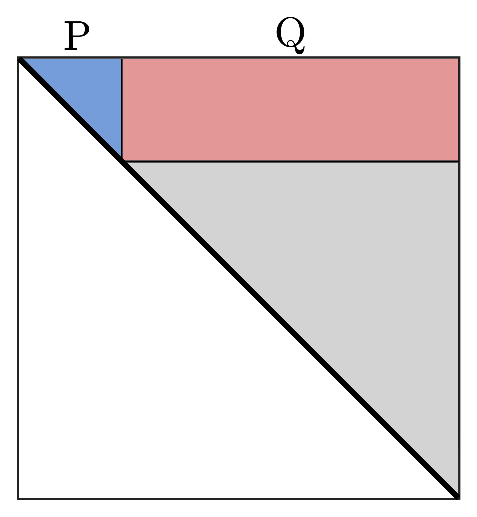
\includegraphics[scale=1]{./figures/CIPT_matrix.eps}
\caption{(First published in Ref. \cite{Dzuba2017}). CIPT matrix structure which is both real and symmetric. The matrix is divided up into three sections for the CIPT calculation. The upper left corner (blue) represents the effective matrix consisting of matrix elements for between states only in set P. The upper middle and right section (red) consists of the matrix elements between states in sets P and Q to be treated perturbatively. The remaining off-diagonal grey matrix elements between states only in set Q are discarded. \label{fig:CIPT_matrix}}
\end{figure}
\section{Relativistic and Radiative effects}
In this work we include the effects of both the Breit interaction \cite{Breit1929, Mann1971} and quantum electrodynamic (QED) radiative corrections (self-energy and vacuum polarisation corrections) \cite{FG2005} for completeness. The Breit interaction which accounts for the magnetic interaction and retardation is included in the zero momentum transfer approximation,
\begin{align}\label{eq:HB}
\hat{H}^B = -\dfrac{\boldsymbol{\alpha}_1 \cdot \boldsymbol{\alpha}_2 + \left(\boldsymbol{\alpha}_1\cdot\textbf{n}\right)\left(\boldsymbol{\alpha}_2\cdot \textbf{n}\right)}{2r}
\end{align}
where $\boldsymbol{\alpha}$ is the Dirac matrix, $\textbf{r}=r\textbf{n}$ and $r$ is the distance between electrons 
denoted by subscripts $1$ and $2$.  Similar to Coulomb interaction, Breit interaction (\ref{eq:HB}) leads to Breit potential
$V_B$ which is added to the HF potential and included into the HF iterations.

The QED radiative corrections due to the Uehling potential $V_U$, and electric and magnetic form-factors 
$V_E $ and $ V_g$  are included via a radiative potential $V_R$~\cite{FG2005},
\begin{align}\label{eq:VR}
V_{R}(r) = V_{U}(r) + V_{g}(r) + V_{E}(r).
\end{align}
It is also included into the HF procedure.
%Both the Breit and effective radiation correction potentials are included  in the Hartree-Fock procedure described above.
Note that iterating  HF equations with Breit and QED potentials $V_B$ and $V_R$ formally lead to inclusion of non-linear
contributions  $V_B^2$, $V_R^2$, etc. which have no physical meaning. We have checks that corresponding contributions
are small and cause no problem. On the other hand, iterating the HF equations with $V_B$ and $V_R$ takes into account
an important relaxation effect~\cite{DF2016} which is first order in $V_B$ or $V_R$ but all-order in Coulomb interaction.
This relaxation effect reduces the size of the Breit or QED correction to the energy up to two times~\cite{DF2016}.
Both, Breit and QED corrections grow with $Z$ faster than first power of $Z$, therefore it is important to check whether
they give significant contributions to the energies of SHE. See section~\ref{sec:DbI} for more discussion. 
\section{Estimation of the accuracy} \label{sec:Accuracy}

Theoretical uncertainty is dominated by incomplete treatment of inter-electron correlations. These correlations can be further separated into core-valence and valence-valence correlations. We will discuss each of these separately. For the SHE calculations, the core includes all states in closed shells
from $1s$ to $5f$ containing one hundred electrons occupying one hundred states.
All other states, including states of the $6d$ and $7s$ shells are treated as
valence states. Only valence states are used in calculation of the CI matrix.
This means that we neglect core-valence correlations. To estimate the corresponding uncertainties, we perform calculations of the energy levels of gold and roentgenium (Rg, $Z$=111). Both these elements have one external electron above a closed $5d$ or $6d$ shell. We perform the calculations using the correlation potential method~\cite{Dzuba1988, DFSS1987_2}. In this method, core-valence correlation corrections are obtained using the electron self-energy operator (correlation potential) $\Sigma$\footnote{Do not confuse this with  the QED self-energy operator which we included using the radiative potential method \cite{FG2005}. This is the many-body self-energy operator, which for example, has been defined in the textbook \cite{LandauStatPhysPart2}. We calculate this operator using a Feynman diagram technique with relativistic Hartree-Fock Green's functions \cite{Dzuba1988}.} calculated by summation of the diagrams in the many-body perturbation theory.  The operator $\Sigma $ is defined by the correlation correction to the energy of the valence electron on the orbital $n$, $\delta E_n = \langle n | \Sigma | n \rangle$.   For the Au and Rg calculations, the upper complete $d$-shell ($5d$ or $6d$) is attributed to the core, and the correlation interaction of the external electron with the core is described by a correlation potential $\Sigma$.   \\

Calculation of $\Sigma$ involves a summation over all core states from
$1s$ to $5d$ for Au or $6d$ for Rg. This summation is strongly dominated by the upper $d$-shell. E.g., the $5d$ shell gives about 90\% of the correlation correction to the energies of the $6s$ and $6p$ valence states of Au, and more than 80\% of the correlation correction to the energies of the $7s$ and $7p$ valence states of Rg (see Table \ref{tab:CPaccuracy}). This is because of the small energy interval between the energies of
the $5d$ (or $6d$) state and the energies of lowest valence states.  Since correlation correction to the energy of the $s$ and $p$ valence states is about 20\%, the effect of neglecting inner-core contributions to the core-valence correlations is about 1 to 2\% of the energy of valence states.

%This appears in the correlation
%potential method via small energy denominator in the expression for $\Sigma$,
%which is this small energy interval.

\begin{table}
\centering
\caption{Removal energies (cm$^{-1}$) for states of external electron of
Au and Rg calculated in different approximations. RHF is relativistic
Hartree-Fock, $\Sigma$($nd$) are Brueckner orbital energies calculated with correlation
potential $\Sigma$, in which summation over core states is limited to $5d$ or
$6d$ shell only. $\Sigma$(all) are the energies calculated with full summation over
core states. \label{tab:CPaccuracy}}
\begin{tabular}{l@{\hspace{0.7cm}}r@{\hspace{0.7cm}}r@{\hspace{0.7cm}}r@{\hspace{0.7cm}}r}
\toprule
\toprule
\multicolumn{5}{c}{Au} \\
  &  \centering    RHF &  $\Sigma$($5d$) &    $\Sigma$(all) &   Expt~\cite{NIST_ASD} \\
  \midrule
$6s_{1/2}$ &  60 179 &  75 539  & 77 878 &  74 409 \\
$6p_{1/2}$ &  29 303 & 36 508  & 37 322 & 37 051 \\
$6p_{3/2}$ &  26 664  & 32 314  & 32 785 & 33 324 \\
$6d_{3/2}$  & 11 929  & 12 423  & 12 439 & 12 457 \\
$6d_{5/2}$ &   11 875  & 12 344 &  12 357 & 12 376 \\
\\
\multicolumn{5}{c}{Rg} \\
    &   \centering  RHF  &    $\Sigma$($6d$) &   $\Sigma$(all)  \\
    \midrule
$7s_{1/2}$  & 83 436 & 101 901 & 106 780 \\
$7p_{1/2}$ &  38 006 &  49 996 &  52 269 \\
$7p_{3/2}$ &  26 550 &  33 659 &  34 685 \\
$7d_{3/2}$  & 11 859 &  12 594 &  12 656 \\
$7d_{5/2}$  & 11 738  & 12 383  & 12 428 \\
\bottomrule
\bottomrule
\end{tabular}
\end{table}

   It is interesting to note that in the second order of many-body perturbation theory, the correlation potential$\Sigma$ always overestimates the value of the correlation correction. This is because it does not include the effect of screening of inter-electron interaction by other atomic electrons. This effect appears in higher orders of perturbation theory. Its proper inclusion leads to very accurate results (see, e.g.~\cite{Dzuba1988, Dzuba2008}).
   
Since in the present work we do not go beyond the second order, we have the fortunate situation where neglecting inner-core contributions to $\Sigma$ has a similar affect on its value as the screening would do. In other words, the effect of neglecting the higher-order perturbative contributions on
the calculated energies partially compensates the effect of neglecting
screening of interelectron interactions. The data in Table \ref{tab:CPaccuracy} show that this is the case at least for the
$6s$ state of Au (and probably for the $7s$ state of Rg) where the correlation correction
is the largest in value. Therefore, it is reasonable to assume that the theoretical uncertainty is dominated by valence-valence correlations. The main source for it is the perturbative treatment of the excited configurations. The best way of estimating the uncertainty is to compare the theoretical and experimental energies for lighter elements. We did this in detail for W~\cite{DBHF2017}, which is the lighter analog of Sg, and for pairs Ta and Db~\cite{LDFDb2018}, and Rn and Og~\cite{LDFOg2018}. As follows from this comparison and from the analysis in Sections \ref{sec:Sg}, \ref{sec:Bh}, the theoretical uncertainty for the energies is on the level of $\sim$ 1000~cm$^{-1}$, sometimes a little higher (e.g.  $\sim$ 2000~cm$^{-1}$ for odd states of Bh). The uncertainty for ionization potentials is on the level of a few percent (see section \ref{sec:SHEIP}).

\section{Comparison of CIPT calculations with experimental results in Ta}
\begin{table}[p!]
\centering
\caption{Comparison of experimental (from ref.\cite{NIST_ASD}) and CIPT spectra and ionisation potential of Ta I. The experimental excitation energies ($E_E$) and Land\'{e} g-factors ($g_E$) are compared to respective CIPT excitation energies ($E_T$) and Land\'{e} g-factors ($g_T$).   The final column is the difference between experimental and theoretical excitation energies $\Delta = E_{E} - E_{T}$. \label{tab:TaComparison}}
\begin{tabular}{cl@{\hspace{0.5cm}}l@{\hspace{0.5cm}}c@{\hspace{0.5cm}}r@{\hspace{0.5cm}}r@{\hspace{0.5cm}}r@{\hspace{0.5cm}}r@{\hspace{0.5cm}}r}
\toprule
\toprule
& & & & \multicolumn{2}{c}{Experimental} & \multicolumn{2}{c}{CIPT} &  \\
\cmidrule{5-6} \cmidrule{7-8}
& Configuration & State & $J$ &  \multicolumn{1}{c}{\parbox{1cm}{ $E_E$ \\ (cm$^{-1}$)}}  &  \multicolumn{1}{c}{$g_E$} &  \multicolumn{1}{c}{\parbox{1cm}{$E_T$ \\ (cm$^{-1}$)} } &  \multicolumn{1}{c}{$g_T$} &  \multicolumn{1}{c}{\parbox{1cm}{$\Delta$ (cm$^{-1}$)} } \\
\midrule
& Even states\\
(1)  &$5d^3 6s^2$ & $^4$F & 3/2 & 0.00 & 0.447 &  0.00 & 0.4373 & \\
(2)  &$5d^3 6s^2$ & $^4$F & 5/2 & 2 010 & 1.031 &  1 652 & 1.0336 & 358 \\
(3)  &$5d^3 6s^2$ & $^4$F & 7/2 & 3 964 & 1.218 & 3 175 & 1.2265 &  789\\
(4)  &$5d^3 6s^2$ & $^4$F & 9/2 & 5 621 & 1.272 & 4 679 & 1.3066 & 942\\
(5)  &$5d^3 6s^2$ & $^4$P & 1/2 & 6 049 & 2.454 & 6 017 & 2.4022 & 32\\
\\
& Odd states\\
(6)  &$5d^3 6s 6p$ & $^6$G$^{\rm_o}$  & 3/2 & 17 385 &  & 17 599 &   0.1719   &  -214\\
(7)  &$5d^3 6s 6p$ & $^2$F$^{\rm_o}$  & 5/2 & 17 994 & 0.732 &  18 225 &   0.7955  & -231\\
(8)  &$5d^2 6s^2 6p$ & $^4$D$^{\rm_o}$  & 1/2 & 18 505 & 0.172 & 18 629 &   0.0716  & -124\\
(9)  &$5d^3 6s 6p$ & $^6$G$^{\rm_o}$  & 5/2 & 19 178 & 0.851 & 19 393 &   0.8551 &  -123\\
(10)  &$5d^2 6s^2 6p$ & $^4$D$^{\rm_o}$  & 3/2 & 19 658 & 1.018 & 19 724 &   0.9389 & -66\\
(11)  &$5d^2 6s^2 6p$ & $^2$S$^{\rm_o}$  & 1/2 & 20 340 & 1.956 & 20 574 &   2.0278 & -233\\
(12)  &$5d^3 6s 6p$ & $^6$G$^{\rm_o}$  & 7/2 & 20 560 & 1.194 & 20 463 &   1.1394 & -97\\
(13)  &$5d^2 6s^2 6p$ & $^2$D$^{\rm_o}$  & 3/2 & 20 772 & 0.812 & 20 796 &     0.8124 & -24\\
(14)  &$5d^2 6s^2 6p$ & $^4$D$^{\rm_o}$  & 5/2 & 21 168 &   & 21 358 &   1.2117 &  -190\\
(15)  &$5d^3 6s 6p$ & $^4$F$^{\rm_o}$ & 3/2 & 21 855 & 0.666 & 22 132 & 0.6773 & -277 \\
(16)  &$5d^2 6s^2 6p$ & $^2$D$^{\rm_o}$ & 5/2 & 22 047 & 1.179 & 21 875 & 1.0838 & 172 \\
(17)  &$5d^2 6s^2 6p$ & $^4$G$^{\rm_o}$  & 7/2 & 22 381 & 1.060 & 22 276 & 1.0377 & 105 \\
(18)  &$5d^3 6s 6p$ & $^6$G$^{\rm_o}$ & 9/2 & 22 682 & 1.231 & 22 285 & 1.2677 & 397 \\
(19)  &$5d^3 6s 6p$ & $^6$F$^{\rm_o}$ & 1/2 & 23 355 & -0.320 & 23 680 & -0.2689 & -325 \\
(20)  &$5d^3 6s 6p$ & $^4$F$^{\rm_o}$ & 5/2 & 23 363 & 1.078 & 23 381 & 1.0766 & -18 \\
(21)  &$5d^2 6s^2 6p$ & $^4$D$^{\rm_o}$ & 7/2 & 23 927 & 1.326 & 23572 & 1.3256 & 355 \\
(22)  &$5d^3 6s 6p$ & $^6$F$^{\rm_o}$ & 3/2 & 24 243 & 1.126 & 24 463 & 1.1018 & -220 \\
(23)  &$5d^3 6s 6p$ & $^6$D$^{\rm_o}$ & 1/2 & 24 517 & 2.888 & 24 907 & 2.9261 & -390 \\
(24)  &$5d^3 6s 6p$ & $^6$D$^{\rm_o}$ & 3/2 & 24 739 & 1.620 & 25 143 & 1.6808& -404 \\
(25)  &$5d^3 6s 6p$ & $^4$F$^{\rm_o}$  & 7/2 & 24 982 & 1.235  & 24 922 & 1.2590 & 60 \\
(26)  &$5d^3 6s 6p$ & $^6$G$^{\rm_o}$ & 11/2 & 25 009 & 1.302 & 24 528 & 1.3366 & 481 \\
(27)  &$5d^3 6s 6p$ & $^6$F$^{\rm_o}$ & 5/2 & 25 181 & 1.239 & 25 267 & 1.2573 & -86 \\
(28)  &$5d^3 6s 6p$ & $^6$G$^{\rm_o}$ & 9/2 & 25 186 &  & 24 733  & 1.2540 & 453 \\
(29)  &$5d^3 6s 6p$ & $^4$D$^{\rm_o}$ & 1/2 & 25 513 & 0.028 & 25 697 & 0.0319  & -184 \\
(30)  &$5d^3 6s 6p$ & $^4$F$^{\rm_o}$  & 9/2 & 25 926 &  1.292 & 25 509 & 1.2970 & 417 \\
(31)  &$5d^2 6s^2 6p$ & $^4$P$^{\rm_o}$ & 5/2 & 26 220 & 1.338 & 26 298 & 1.2923 & -78 \\
(32)  &$5d^3 6s 6p$ & $^4$D$^{\rm_o}$ & 3/2 & 26 364 & 1.393 & 26 678 & 1.2676 & -314 \\
(33)  &$5d^3 6s 6p$ & $^6$F$^{\rm_o}$  & 7/2 & 26 586 & 1.356  & 26 299 & 1.315 & 287 \\
(34)  &$5d^2 6s^2 6p$ & $^4$P$^{\rm_o}$ & 3/2 & 26 590 & 1.576 & 26 759 & 1.6833 & -169\\
(35)  &$5d^3 6s 6p$ & $^6$D$^{\rm_o}$ & 5/2 & 26 795 & 1.416 & 26 815 & 1.4086 & -20 \\
(36)  &$5d^2 6s^2 6p$ & $^4$P$^{\rm_o}$ & 1/2 & 26 866 & 2.650 & 27 094 & 2.6189 & -228\\
(37)  &$5d^3 6s 6p$ &  $^4$F$^{\rm_o}$   & 7/2 & 26 960 & 1.223  & 26 787 & 1.2390 & 173 \\
(38)  &$5d^3 6s 6p$ & $^6$F$^{\rm_o}$  & 9/2 & 27 733 &  1.390 & 27 279 & 1.3590 & 454 \\
(39)  &$5d^3 6s 6p$ & $4$D$^{\rm_o}$   & 7/2 & 27 781 & 1.374  & 27 643 & 1.4658 & 138 \\
(40)  &$5d^3 6s 6p$ & $^6$G$^{\rm_o}$ & 11/2 & 27 783 & 1.351 &  27 376 & 1.350  & 407\\
(41)  &$5d^3 6s 6p$ & $^4$D$^{\rm_o}$ & 5/2 & 28 134 & 1.394 & 28 337 & 1.3665 & -203 \\
(42)  &$5d^3 6s 6p$ & $^4$G$^{\rm_o}$   & 7/2 & 28 183 & 1.115  & 27 970 & 1.0421 & 213 \\
(43) &$5d^3 6s 6p$ & $^2$P$^{\rm_o}$   & 3/2 & 28 689 & 1.356  & 28 693 & 1.3052  & -4 \\
(44)  &$5d^3 6s 6p$ & $^6$D$^{\rm_o}$  & 9/2 & 28 767 &  1.337 & 28 414 & 1.4106 & 353 \\
(45)  &$5d^3 6s 6p$ & $^6$F$^{\rm_o}$ & 5/2 & 28 862 & 1.247 & 28 868 & 1.2678 & -6 \\
(46)  &$5d^3 6s 6p$ & $^6$D$^{\rm_o}$ & 1/2 & 29 902 & 2.994 & 30 323 & 2.9971 & -421 \\
\\
& Ta I ionisation potential \\
(47)  &$5d^3 6s$& $5$F & 1 & 60 891 & 0.000 & 61 073 &    0.0235 &  -182\\
\bottomrule
\bottomrule
\end{tabular}
\end{table}

To demonstrate the accuracy of the CIPT method we compare the theoretical and experimental spectra of Ta~I. As Ta lies in the same group but one period lower, we believe theoretical accuracy of the CIPT Ta spectrum would indicate the accuracy we can expect for Db. Electron states of neutral Ta have an open $5d$ shell, its ground state configuration is [Xe]$4f^{14}5d^3 6s^2$. As the $6s$ electrons are easily excited, we should treat the atom as a system with five external electrons. Note that a slightly more complicated atom, tungsten, which has one more external electron, was already successfully studied using the CIPT method~\cite{DBHF2017}. Therefore, we expect similar or better accuracy for Ta. For low lying even parity states of Ta we used the basis states of the $5d^3 6s^2$, $5d^4 6s$ and $5d^5$  configurations in the effective CI matrix. All other configurations, which were obtained by exciting one or two electrons from these configurations, were included perturbatively. Similarly for the odd parity states we used the states of the $5d^3 6s 6p$, $5d^2 6s^2 6p$ configurations in the effective CI matrix, while other configurations are included perturbatively.

In Table \ref{tab:TaComparison} we present the comparison between experimental excitation energies and $g$-factors and those calculated by the CIPT method.  We present a significant number of odd parity states to demonstrate the accuracy these states particularly towards the end of the optical region. This is because the most promising measurements are strong optical electric dipole (E1) transitions between the ground state and excited states of different parity. 
It is important to include as many of these transitions as possible. To identify the correct states for comparison with experiment 
we use the experimental and theoretical Land\'{e} $g$-factors. When experimental $g$-factors were not available we used the next sequential state in the theoretical calculations. There was excellent agreement between the experimental and CIPT $g$-factors with maximum difference between theory and experiment $\Delta g \approx 0.1$. This is sufficient accuracy for identification of the states.
%the only significant difference for the odd state $J=1/2$ at $18 505$ cm$^{-1}$.  

There is good agreement between the experimental and theoretical excitation energies particularly for the low-lying odd parity 
states which are important for measuring the electric dipole transitions (see Section \ref{sec:E1transitions}). For the odd parity
states the largest discrepancy in energy was $\Delta = 453$ cm$^{-1}$ with most states having $|\Delta| \approx 100-400$ 
cm$^{-1}$. The main source of the difference between theory and experiment is incomplete treatment of the correlations,
which mostly comes from two factors. We neglect core valence correlations and off-diagonal matrix elements between
highly excited states. This is the price we have to pay to be able to perform the calculations for a
complicated system with five external electrons. There are some smaller factors, like cutting basis at $l_{max}=4$, 
ignoring triple excitations, etc.
%Our calculations also supported the existence of the $J=11/2$ level at $E_E=  27 783$ cm$^{-1}$ which is listed as ambiguous \cite{NIST_ASD}.  
For the CIPT calculations of the Db I spectrum we expect a similar accuracy as seen in Ta~I due to the similar electronic structure.\\


\chapter{Energy Levels of superheavy elements}

\chapter{Electric dipole transitions}

\chapter{Isotope shifts in super heavy elements}

\section{Db I} \label{sec:DbI}

Dubnium was first synthesized in 1968 and the current longest living isotope is $^{268}$Db with a halflife of $\approx 30 $ hrs 
\cite{Schadel2012, Oganessian2005}. This long lifetime relative to other SHEs makes future experiments promising. 
There is limited experimental and theoretical data for Db with the majority being chemical properties~\cite{Schadel2012,
 Fricke1975}.  An estimation of the ionisation potential has been performed for Db in~\cite{Dzuba2016} using a relativistic 
 Hartree-Fock  method with semi-empirical corrections introduced to simulate the effect of correlations.

For the CIPT calculations of Db~I we use the same parameters as for the Ta~I calculations in Section \ref{sec:TaI}. In the $V^{N-1}$ approximation discussed in Section \ref{sec:CIPT} we remove a $7s$ electron in the initial Hartree-Fock
calculations and in the calculation of the single-electron basis states.
 The Db~I ground state is [Rn]$5f^{14}6d^3 7s^2$ which is similar to Ta I with different principle quantum numbers. For calculation of the even parity states we populated the effective CI matrix with the states of the $6d^3 7s^2$,  $6d^4 7s$ and $6d^5$ configurations. All higher states are obtained through single and double excitations of these states and are included perturbatively. Similarly for  the states of odd parity the effective matrix contains states of the  $6d^3 7s 7p$, $6d^2 7s^2 7p$ and $6d^4 7p$ configurations. Other configurations are included perturbatively. For the ion  we use the states of the $6d^3 7s$, $6d^2 7s^2$ and $6d^4$ configurations.  Both Breit and radiative corrections are expected to be larger in SHE compared to lighter elements and therefore are included in Table~\ref{table:DbISpectrum}. In Table~\ref{table:DbISpectrum} we present the excitation energies of Db using the CIPT method. To demonstrate the affect of  Breit and QED corrections we performed four separate calculations,
first with no Breit or QED corrections, second with only Breit correction included, then with QED included but no Breit, and finally,
with both corrections included (see Table~\ref{table:DbISpectrum}).
\begin{table*}[p!]
\begin{adjustwidth}{-1.3cm}{-1.3cm}
\centering 
\caption{Spectrum for the low lying energy levels of Db I and Db II using the CIPT method. Here $E_{NC}$ are the excitation energies when neither Breit nor radiative corrections are included in the calculations, $\Delta_B$ and $\Delta_R$ are the changes in energy from $E_{NC}$ when Breit and radiative corrections are included respectively. The final energy $E$ is the excitation spectrum when both Breit and radiative corrections are included \textit{ab initio}. The accuracy of these levels is expected to be similar to Ta I presented in Table \ref{tab:TaComparison}. (Originally published in \cite{LDFDb2018}). \label{table:DbISpectrum}} 
\begin{tabular}{cllcrrrrr}
\toprule
\toprule
  & & & & \multicolumn{4}{c}{Excitation energy} &\\
  \cmidrule{5-8}
& \parbox{2cm}{Major \\ Configuration} & State & $J$ & \parbox{2cm}{CIPT with \\ no Breit or QED \\ $E_{NC}$ \\ (cm$^{-1}$)} & \parbox{2cm}{Breit \\ correction \\ $\Delta_B$ \\ (cm$^{-1}$)} & \parbox{2cm}{QED \\ corrections \\$\Delta_R$\\ (cm$^{-1}$)} &  \parbox{2cm}{Total\\ $E$ \\ (cm$^{-1}$)} & \parbox{1.5cm}{Land\'{e} \\g-factor} \\ 
\midrule
& Even States \\
(1)  &   $6d^3 7s^2$  &  $^4$F  &  $3/2$ & 0 & 0 & 0 & 0 & 0.554 \\ 
(2) &   $6d^3 7s^2$  &  $^4$F &  $5/2$  &  4 072 & -77 & 21 & 4 016 & 1.043 \\ 
(3)  &  $6d^3 7s^2$  &  $^2$F &  $7/2$  &  6 595 & -100 & 31 & 6 527 & 1.170 \\ 
(4)  &  $6d^3 7s^2$  &  $^2$S  & $1/2$ &  7 691 &  -73  &  16 & 7 634 & 2.058 \\ 
(5)  &  $6d^3 7s^2$  &  $^4$G &  $9/2$ &  8 076 & -92 &  33 & 8 017 & 1.191 \\ 
&  Odd States \\
(6) & $6d^2 7s^2 7p$  &  $^2$F$^{\rm_o}$  & $5/2$ &  6 255 & 213 &  123 & 6 591 & 0.739 \\ 
(7)  & $6d^2 7s^2 7p$  &  $^2$D$^{\rm_o}$  & $3/2$ &  11 240 & 156 &  87 & 11 483 &  0.633 \\ 
(8)  &   $6d^2 7s^2 7p$  &  $^2$P$^{\rm_o}$ &  $1/2$ &  12 642 & 140 &  84  & 12 869 & 1.308 \\ 
(9)  &  $6d^2 7s^2 7p$  &  $^4$G$^{\rm_o}$ &  $7/2$  &  13 645 &  116 &  147 & 13 909 & 1.023 \\ 
(10)   &  $6d^2 7s^2 7p$  &  $^4$F$^{\rm_o}$  & $5/2$ &  13 873 & 113  &  132 & 14 117 & 1.067 \\ 
(11)   &  $6d^2 7s^2 7p$  &  $^2$P$^{\rm_o}$  & $1/2$ &  14 516 & 96  &  88  & 14 705 & 0.995 \\ 
(12)   &  $6d^2 7s^2 7p$  &  $^6$F$^{\rm_o}$  & $3/2$ &  14 572 & 105 & 96  & 14 772 & 1.111 \\ 
(13)   &  $6d^2 7s^2 7p$  &  $^4$F$^{\rm_o}$ &  $5/2$ &  17 493 & 78 &76  & 17 647 & 1.111 \\ 
(14)  &  $6d^2 7s^2 7p$  &  $^4$G$^{\rm_o}$  & $9/2$ &  18 596 & 80 &  144  & 18 820  & 1.145 \\ 
(15)  & $6d^3 7s 7p$  &  $^2$D$^{\rm_o}$  & $3/2$ &  19 379 & 62 &  -3  & 19 438 & 0.701 \\ 
 (16)  &  $6d^2 7s^2 7p$  &  $^4$F$^{\rm_o}$ &  $7/2$  &  20 462 & 53 & 134 & 20 649  & 1.203 \\ 
(17)  &  $6d^2 7s^2 7p$  &  $^6$F$^{\rm_o}$  & $3/2$ &  21 706 & 56  & 50 & 21 811 & 1.073 \\ 
(18)  &  $6d^2 7s^2 7p$  &  $^4$D$^{\rm_o}$ &  $1/2$ &  22 123 & 72  & 93 & 22 284 & 0.078 \\ 
(19)   &  $6d^2 7s^2 7p$  &  $^4$F$^{\rm_o}$ &  $5/2$ &  22 204 & 35  & 54 & 22 292 & 1.110 \\ 
(20)  &  $6d^2 7s^2 7p$  &  $^2$D$^{\rm_o}$  & $3/2$ &  23 003 & 39 & 22 & 23 067 & 0.697 \\ 
(21)  &  $6d^2 7s^2 7p$  &  $^2$F$^{\rm_o}$ &  $7/2$  &  23 221 & 37   & 133 & 23 390 & 1.102 \\ 
(22)  &  $6d^3 7s 7p$  &  $^4$F$^{\rm_o}$  & $5/2$ &  23 910 &  4 &  -2 & 23 913 & 0.948 \\ 
(23) &   $6d^2 7s^2 7p$  &  $^2$P$^{\rm_o}$ &  $3/2$ &  24 622 & 2  &  119  & 24 743  & 1.372 \\ 
(24)  &   $6d^2 7s^2 7p$  &  $^2$G$^{\rm_o}$  & $9/2$ &  24 915&  27  & 133 & 25 074 & 1.111 \\ 
 (25)  & $6d^3 7s 7p$  &  $^2$F$^{\rm_o}$ &  $7/2$  &  25 458 & 9  & 17  & 25 480 & 1.152 \\ 
(26) &   $6d^2 7s^2 7p$  &  $^4$F$^{\rm_o}$ &  $5/2$ &  25 510 & 5   & 73 & 25 589 & 1.031 \\ 
(27)   & $6d^2 7s^2 7p$  &  $^2$F$^{\rm_o}$ &  $7/2$ &  26 538 & -4   &  78 & 26 612 & 1.172 \\ 
(28)   &  $6d^2 7s^2 7p$  &  $^2$S$^{\rm_o}$ &  $1/2$ &  27 435 & -10   &  49 & 27 479 & 1.663 \\ 
(29)  &   $6d^2 7s^2 7p$  &  $^2$F$^{\rm_o}$ &  $7/2$  &  27 662 & -23   & 24  & 27 666 & 1.128  \\ 
(30)  &  $6d^2 7s^2 7p$  &  $^4$D$^{\rm_o}$ &  $3/2$ &  27 589 & -5   & 114 & 27 697  & 1.147 \\ 
(31)  &  $6d^2 7s^2 7p$  &  $^4$G$^{\rm_o}$ &  $9/2$ &  27 885 & -13   &  118 & 27 990 & 1.173 \\ 
(32)   & $6d^2 7s^2 7p$  &  $^2$D$^{\rm_o}$ &  $5/2$ &  28 162 & -25  & 75 & 28 211  & 1.130 \\ 
(33)    &  $6d^2 7s^2 7p$  &  $^4$P$^{\rm_o}$ &  $3/2$ &  29 183 & 1  & 74 & 29 259 & 1.659 \\ 
(34)  & $6d^2 7s^2 7p$  &  $^4$G$^{\rm_o}$ &  $11/2$ &  29 669 & -45 & 103 & 29 669 & 1.254 \\ 
(35)  & $6d^3 7s 7p$  &  $^6$G$^{\rm_o}$ &  $9/2$ &  29 946 & -75  & -87 & 29 784 & 1.254 \\ 
(36)  &   $6d^2 7s^2 7p$  &  $^6$F$^{\rm_o}$  & $5/2$ &  29 734 &  -25  & 174  & 29 821 & 1.343 \\ 
(37) &  $6d^3 7s 7p$  &  $^4$D$^{\rm_o}$ &  $1/2$ &  29 886 & -24  &  -33  & 29 832 & 0.220 \\ 
(38)  &  $6d^2 7s^2 7p$  &  $^2$F$^{\rm_o}$  &  $7/2$ &  30 474 & -29  & 97 & 30 541  & 1.161 \\ 
 & Db II states\\
(39)  &   $6d^2 7s^2$  &  $^3$F &  $2$ & 56 546 & 48 & 139 & 56 733 & 0.731 \\ 
(40)  &   $6d^2 7s^2$  &  $^3$S &  $0$ & 62 673 & -13 & 119 & 62 778 & 0.000 \\ 
(41)  &   $6d^2 7s^2$  &  $^3$F &  $3$ & 62 952 & -45 & 176 & 63 083 & 1.083 \\ 
(42)  &   $6d^2 7s^2$  &  $^3$D &  $2$ & 65 122 & -62 & 120 & 65 179 & 1.250 \\ 
(43)  &   $6d^2 7s^2$  &  $^3$P &  $1$ & 65 587 & -79 & 113 & 65 620 & 1.467 \\ 
(44)  &   $6d^2 7s^2$  &  $^5$G &  $4$ & 67 466 & -83 & 189 & 67 572 & 1.120 \\ 
\bottomrule 
 \bottomrule 
\end{tabular} 
\end{adjustwidth}
\end{table*}

Comparing the Db~I spectrum in Table~\ref{table:DbISpectrum} to the Ta~I spectrum in Table~\ref{tab:TaComparison} we see there are some notable differences. While the order of even parity states has remained the same relative to each other,  the order of the odd states has been significantly altered with the first $2F^{\rm_o}_{5/2}$ state being significantly lowered in the spectrum. Another thing to note is that the odd parity excitations are typically $6d \rightarrow 7p$ as opposed to the Ta excitation $6s \rightarrow 6p$. This can be explained by relativistic effects where the $7s$ electrons are more tightly bound than the $6d$ electrons in contrast to the $5d$ and $6s$ electrons in Ta \cite{Schwerdtfeger2014}. These relativistic effects also cause the $6d$ electron to be ionised in Db instead of the $7s$ electron. This may result in significantly different chemical properties in Db compared to Ta. \\

\begin{figure}[tb]
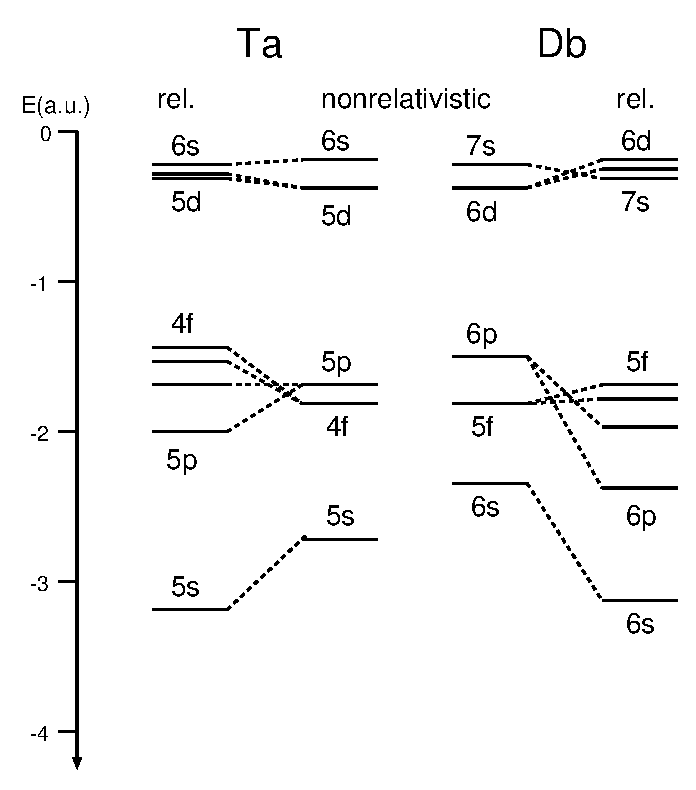
\includegraphics[scale=0.7]{./figures/el.eps}
\caption{Hartree-Fock energies of upper core states of Ta and Db calculated in non-relativistic and relativistic 
approximations.}
\label{f:el}
\end{figure}
To understand the difference between the atoms it is instructive to look at the Hartree-Fock energies and electron 
densities calculated in non-relativistic and relativistic approximations. Fig.~\ref{f:el} shows energies of the upper
core states of Ta and Db. The spectra are very similar. Relativistic energy shifts are larger for Db as expected and
the most noticeable difference cause by this shift is the change of the order of the $6d$ and $7s$ states which leads 
to the  change of the dominant configurations in low odd states of Db as discussed above.  However, the absolute
shift of the energies is small. It changes the order of the states because they are very close in the non-relativistic
calculations. This change in the Hartree-Fock spectra caused by relativistic effects suggests that the differences 
in the spectra of neutral Ta and Db are mostly due to relativistic effects while correlation corrections are
similar. This means that the accuracy of the calculations should also be similar for Ta and Db.
This can be further illustrated by comparing the electron densities of the atoms calculated in non-relativistic and relativistic
approximations (see Fig.~\ref{f:ro}). Examining the densities one can see the following:
(a) There are four peaks for Ta and five for Db. They correspond to shells with principal quantum numbers from 1 to 4 for
Ta and 1 to 5 for Db. Electrons in higher shells are distributed over larger distances and their density does not form a peak.
(b)  Relativistic effects pull inner electrons towards the nucleus but have little effect on outer electrons.
(c) The densities at large distances ($r>a_B$), where external electrons are located, are very similar.
This is another indication that correlations are likely to be similar.  To check this we performed another test. We
compared the contribution of high energy states (second term in (\ref{e:PT})) to the energies of Ta and Db.
It turns out that the corrections to the energies of even states of Ta and Db differ by 2\% only while corrections to 
the energies of odd states of Db about 30\% larger than those of Ta. This means the uncertainty in the calculations for these
states might also be larger for Db. Therefore, it seems to be reasonable to increase estimated uncertainty from 
$ \sim 400$~cm$^{-1}$ for Ta to $ \sim 500$~cm$^{-1}$ for Db.

\begin{figure}[tb]
\includegraphics[scale=0.45]{./figures/ro.eps}
\caption{Electron density normalized to one ($\int \rho dV = 1$) of Db and Ta  calculated in non-relativistic (solid line)
and relativistic (dotted line) approximations.}
\label{f:ro}
\end{figure}
From Table~\ref{table:DbISpectrum} we see that the effect of both the Breit interaction ($\Delta_B$) and radiative corrections 
($\Delta_R$)  is small and lies within the accuracy of our CIPT method. As it was discussed in previous section the main
source of the uncertainty of the calculations comes from incomplete treatment of the correlations and it is $ < 500$~cm$^{-1}$
for Ta. It is expected to be similar for Db. On the other hand, the maximum value of the sum of Breit and QED corrections for 
Db is $\sim 300$~cm$^{-1}$ while for most of the states it is $< 200$~cm$^{-1}$ (see Table~\ref{table:DbISpectrum}).
It is interesting that the Breit and QED effects do not correlate with each other. This can be seen by summing the two  
corrections and the calculated energy with no  corrections included ($E_{NC}$). This energy is very close to states in 
the spectrum which include both corrections simultaneously,
\begin{align*}
E \approx E_{NC} + \Delta_B + \Delta_R.
\end{align*}
Including both Breit and QED effects simultaneously will introduce new terms which are second order in perturbations of the interactions. Since both corrections are small these new terms will be negligible.
To test the consistency of our method we calculated the spectrum of Db~I using the $V^{N-1}$ approach removing a $6d$ electron for the frozen core potential. In these calculations we obtained a similar spectrum within the accuracy of our calculations.

During completion of our work another paper on calculation of the Db spectrum appeared~\cite{Geddes2018}.
The calculations are done with a different implementation of a very similar method. The difference between the results 
of two papers seems to be larger than the uncertainty of our calculations. However, if we accept the difference between 
theory and experiment for Ta in~\cite{Geddes2018} as an estimation of the uncertainty of their calculations, the results
are consistent.

We are not aware of any other calculations of the Db spectrum apart from the calculations of IP. Our value 56744~cm$^{-1}$ is in good agreement with the Hartree-Fock number 55000(7000)~cm$^{-1}$~\cite{Dzuba2016} and
coupled cluster number 55590~cm$^{-1}$~\cite{BorschevskyPC}. Note that the IP of Db is significantly smaller than the IP
of Ta (IP(Ta)=60891~cm$^{-1}$, see previous section) which is another indication of possible different chemical properties. 

\section{Electric dipole transitions and isotope shift} \label{sec:E1transitions}

Due to the current low production rate of dubnium and other SHEs, broad spectroscopic scans are unfeasible for current experimental methods. Therefore experimental searches need to be assisted with theoretical predictions of the strongest lines specifically for optical electric dipole (E1) transitions. In this work we calculate and present the E1 transition amplitudes for the major optical  transitions between the ground state and the  lowest lying odd parity states for each Ta~I and Db~I. It should be noted that there is no published data for the E1 transitions for either Ta~I or Db~I and therefore we present the E1 transition amplitudes ($A_{E1}$)  and transition probabilities ($T_{E1}$) for both atoms. \\

To calculate the E1 transition amplitudes $A_{E1}$ we use the self-consistent random-phase approximation (RPA) to simulate the atom in an external electromagnetic field. This results in an effective electric dipole field for the electrons. The E1 transition amplitude for a transition between states $a$ and $b$ is given by $A_{E1} = \left< b || \hat D + \delta V || a\right>$ where $|a>$ and $|b>$ are the many electron wavefunctions calculated in the CIPT method above, $\hat D$ is the electric dipole operator acting on external electrons, $\delta V$ is the correction to the self-consistent Hartree-Fock potential of atomic core caused by photon electric field. For a more in depth discussion on this method refer to ref. ~\cite{Dzuba2018}. \\

The E1 transition rates are calculated using (in atomic units),
\begin{align*}
T_{E1} = \dfrac{4}{3}\left(\alpha \omega\right)^3\dfrac{ A_{E1}^2}{2J + 1}
\end{align*}
where $J$ is the angular momentum of the odd parity state, $\alpha$ is the fine structure constant and $\omega$ is the frequency of the transitions in atomic units. All calculations obey the selection rules for E1 transitions, a change in parity and change in angular momenta $|\Delta J| \leq 1 $. We present the E1 transitions for Ta I and Db I in Table \ref{table:E1Amplitudes}.\\

\begin{table*}[t!] 
\centering
\caption{Allowed electric dipole transitions between the  ground states of Ta I ($^4F_{3/2}$) and its low lying odd parity states.  The numbers next to the states correspond to the numbered spectra in Tables \ref{tab:TaComparison}. The transition amplitudes $D_{E1}$ are in atomic units. (Originally published in \cite{LDFDb2018}) \label{table:E1Amplitudes} }
\begin{tabular}{cl@{\hspace{0.75cm}}r@{\hspace{0.75cm}}r@{\hspace{0.75cm}}}  % @{} adds extra padding to the columns 
\toprule
\toprule
\multicolumn{4}{c}{Ta I}  \\ \\
 & State &   \multicolumn{1}{c}{\parbox{1cm}{$D_{E1}$ \\ (a.u)}} & \parbox{1.5cm}{$A_{E1}$ \\ $(\times 10^{6} \ \text{s}^{-1})$ } \\
\midrule
 (6) & $^6$G$^{\rm_o}_{3/2}$  & -0.270   & 0.194   \\
(7) & $^2$F$^{\rm_o}_{5/2}$  & 0.214 &  0.090   \\
(8) & $^4$D$^{\rm_o}_{1/2}$   & -0.641   & 2.64  \\
 (9) & $^6$G$^{\rm_o}_{5/2}$  & -0.434   & 0.449   \\
 (10) & $^4$D$^{\rm_o}_{3/2}$   & 0.149   &  0.0856   \\
 (11) &$^2$S$^{\rm_o}_{1/2}$    & -0.107  & 0.0973   \\
 (13) &$^2$D$^{\rm_o}_{3/2}$    & 0.495   & 1.12  \\
 (14) &$^4$D$^{\rm_o}_{5/2}$   & -0.200   &  0.128    \\
 (15) &$^4$F$^{\rm_o}_{3/2}$  & -0.360   & 0.688   \\
 (16) &$^2$D$^{\rm_o}_{5/2}$    & 0.069   & 0.0160   \\
 (19) &$^6$F$^{\rm_o}_{1/2}$   &   0.019   & 0.00446  \\
 (20) &$^4$F$^{\rm_o}_{5/2}$   &  -0.094   & 0.0381  \\
 (22) &$^6$F$^{\rm_o}_{3/2}$  & 0.007   & 0.000412  \\
 (23) &$^6$D$^{\rm_o}_{1/2}$    & -0.073   & 0.0795 \\
 (24) &$^6$D$^{\rm_o}_{3/2}$ & -0.249   & 0.477 \\
 (27) &$^6$F$^{\rm_o}_{5/2}$   & -0.356   & 0.683   \\
 (29) &$^4$D$^{\rm_o}_{1/2}$   &  0.282   & 1.34 \\
 (31) &$^4$P$^{\rm_o}_{5/2}$ & 0.202   & 0.248 \\
 (32) &$^4$D$^{\rm_o}_{3/2}$   & 0.405   & 1.53    \\
 (34) &$^4$P$^{\rm_o}_{3/2}$   &  -0.063   & 0.0377 \\
 (35) &$^6$D$^{\rm_o}_{5/2}$  & 0.338   & 0.741   \\
 (36) &$^4$P$^{\rm_o}_{1/2}$    & -0.066   & 0.0859  \\
 (41) &$^6$D$^{\rm_o}_{5/2}$  & -0.278   & 0.583  \\
 (43) & $^2$P$^{\rm_o}_{1/2}$  &  -0.295   & 1.04  \\
\bottomrule
\bottomrule
\end{tabular}
\end{table*}

\begin{table*}[t!] 
\centering
\caption{Allowed electric dipole transitions and associated isotope shift parameters $a$ and $F$  between the  ground state of Db I ($^4F_{3/2}$) and its low lying odd parity states.  The numbers next to the states correspond to the numbered spectra in Table \ref{table:DbISpectrum}. The transition amplitudes $D_{E1}$ are in atomic units. The isotope shift calculation was performed for $^{268}$Db ($\left<r^{2}\right>_{268} = 36.770$ fm$^2$) and $^{289}$Db ($\left<r^{2}\right>_{289}=38.470$ fm$^2$). (Originally published in \cite{LDFDb2018}) \label{table:E1Amplitudes} }
\begin{tabular}{cl@{\hspace{0.75cm}}r@{\hspace{0.75cm}}r@{\hspace{0.75cm}}|r@{\hspace{0.5cm}}r@{\hspace{0.5cm}}r@{\hspace{0.5cm}}r}  % @{} adds extra padding to the columns 
\toprule
\toprule
\multicolumn{7}{c}{Db I} \\ \\
& State &   \parbox{1.5cm}{$D_{E1}$ \\ (a.u)} & \parbox{1.5cm}{$A_{E1}$ \\ $(\times 10^{6} \ \text{s}^{-1})$  } &  \parbox{1cm}{$a  $ (cm$^{-1}$)} & \parbox{1.5cm}{$F $ \\ (cm$^{-1}$/fm$^{2}$)} &  \multicolumn{1}{c}{\parbox{1cm}{$\tilde{F} $ \\ (cm$^{-1}$) }} \\
\midrule
 (6) & $^2$F$^{\rm_o}_{5/2}$  &   0.631  & 0.0385 & 32.16 & 3.11 & 23.78  \\
 (7)  & $^2$D$^{\rm_o}_{3/2}$ & 1.53  &  1.80 & 18.70 & 1.81 & 13.83 \\
(8) &  $^2$P$^{\rm_o}_{1/2}$  & 0.558 & 14.05 & 1.43 & 10.98 \\
 (10) & $^4$F$^{\rm_o}_{5/2}$    & -0.531 &  0.268 & 27.33 & 2.64 & 20.21  \\
 (11) & $^2$P$^{\rm_o}_{1/2}$    & 0.384 & 0.476 & 15.78 & 1.52 & 11.67 \\
(12)  & $^6$F$^{\rm_o}_{3/2}$ & 0.180 &  0.0527 & 14.93 & 1.44 & 11.04 \\
 (13) & $^4$F$^{\rm_o}_{5/2}$  &    -0.339 & 0.213 & 8.39 & 0.81 & 6.21 \\
 (15) & $^2$D$^{\rm_o}_{3/2}$  &   -0.343  & 0.437 & -18.84 & -1.82 & -13.93   \\
(17)  & $^6$F$^{\rm_o}_{3/2}$  &    1.22  & 7.85 & -0.33 & -0.03 & -0.24 \\
 (18) & $^4$D$^{\rm_o}_{1/2}$  &    0.0968 & 0.105 & 13.58 & 1.31 & 10.04 \\
 (19) & $^4$F$^{\rm_o}_{5/2}$ &    -0.163 & 0.0996& -1.54 & -0.51 & -1.14 \\
 (20) & $^2$D$^{\rm_o}_{3/2}$  &    0.784 & 3.83 & -4.88 & -0.47 & -3.61 \\
 (22) & $^4$F$^{\rm_o}_{5/2}$  &    -1.01 & 4.70  & -19.24 & -1.86 & -14.23 \\
 (23)  & $^2$P$^{\rm_o}_{3/2}$  &   -0.150 & 0.173 & 16.75 & 1.62 & 12.38 \\
 (26) & $^4$F$^{\rm_o}_{5/2}$  &    -0.890 & 4.49  & 6.22 & 0.60 & 4.60 \\
 (28) & $^2$S$^{\rm_o}_{1/2}$ &     -0.570 & 6.83 & -4.42 & -0.43 & -3.27 \\
 (30) & $^4$D$^{\rm_o}_{3/2}$ &   -0.114 & 0.139 & 16.04 & 1.55 & 11.86  \\
 (32) & $^2$D$^{\rm_o}_{5/2}$ &  0.228 & 0.393 & 3.31 & 0.32 & 2.45 \\
 (33)  & $^4$P$^{\rm_o}_{3/2}$ &   -0.388 & 2.01 & 6.68 &  0.64 & 4.94 \\
 (36) & $^6$F$^{\rm_o}_{5/2}$ &    -0.0174   & 0.00270 & 14.86 & 1.44 & 10.99 \\
 (37)  & $^4$D$^{\rm_o}_{1/2}$  &   1.49 & 59.7 & -28.14 & -2.72 & -20.81 \\
\bottomrule
\bottomrule
\end{tabular}
\end{table*}

For Db from Table~\ref{table:E1Amplitudes} we see that the  transition between the ground state and the odd parity state $^4$F$_{3/2} \rightarrow ^4$D$^{\rm_o}_{1/2}$ with has the largest transition rate $T_{E1} = 59.7 \times 10^{6}$ s$^{-1}$ with an energy difference 29 886 cm$^{-1}$. The rate of this transition is an order of magnitude lower than the recently measured transition in No \cite{Laatiaoui2016} and calculated in \cite{Borschevsky2007, Indelicato2007, Liu2007} however the level is at a similar energy which may be promising for future experiments on Db. Other promising transitions from the ground state are to states (7), (17), (20), (22), (33) although the rate of these transition are an order of magnitude lower.  
Large E1 amplitudes can probably found when configuration mixing allows for significant contribution of the 
$7p \rightarrow 7s$ transition as opposed to the  $7p \rightarrow 6d$ transition. This is especially clear for the 
$^4$F$_{3/2} \rightarrow ^4$D$^{\rm_o}_{1/2}$ transition considered above.


%A reason for these large E1 amplitudes  could be due to the larger contribution of the $7p \rightarrow 7s$ transition as opposed to the more suppressed $7p \rightarrow 6d$ transition.

Finally, we calculate isotope shift for Db. Isotope shift is important since it helps to obtain information about
nuclei of SHE when frequencies of the transitions are measured for several isotopes. It can also be used 
to predict the spectra of other isotopes, in particular the spectrum of the hypothetically stable neutron-rich 
isotopes with ``magic'' number of neutrons $N=184$. This may help in search for such isotopes.

Isotope shift of SHE elements is strongly dominated by volume shift (also known as ``field shift'' in literature). We calculate it by varying nuclear radius in 
computer codes. We present results in two different forms. First is given by~\cite{DFW17}
\begin{align*}
\delta \nu &= E_{2} - E_{1} = a\left(A_{2}^{1/3} - A_{1}^{1/3}\right),
\end{align*}
where $A_1$ and $A_2$ are atomic numbers for two isotopes ($A_2>A_1$) and $a$ is the parameter which
comes from the calculations. This form is convenient for prediction of the spectra of heavier isotopes. It is motivated by the relativistic dependence of the volume shift on the nuclear radius, $R_N$, which is proportional to $R_N^{2\gamma}$ where $\gamma = \sqrt{1 - (Z\alpha)^2}$. For  Db  $R_N^{ 2\gamma}  \approx R_{N}^{1.28}$ and using the large scale trend for nuclear radii $R_N \propto A^{1/3}$  the volume shift can be approximated by $\propto A^{1/3}$. This nuclear radius approximation is valid for large scale trends in $A$ where nuclear shell fluctuations are suppressed \cite{Angeli2013, DFW17}, this is applicable for our Db I calculations as $A_1$ and $A_2$ are not neighboring isotopes.

Another form for the isotope shift is the standard formula related the change of atomic frequency to the change
of nuclear radius
\begin{align*}
\delta \nu &= F\delta \left<r^{2}\right>.
\end{align*}
This formula is convenient for extraction of the nuclear radius change from the isotope shift measurements.
The values of the $a$ and $F$ parameters for strong electric dipole transitions of Db are presented in 
Table~\ref{table:E1Amplitudes}.


\chapter{$Z=106-112$}

In this work we present the low-lying odd and even states of SHE $Z=106$-$109$ including the allowed E1 transition amplitudes and rates from the ground state to odd parity states. We also calculate the ionization potential and isotope shift parameters for these elements.\\

The paper progresses as follows; in Section \ref{sec:CIPT} we give a brief overview of the CIPT technique and how we implement it for the SHE. In Section \ref{sec:Accuracy} we discuss the accuracy of the calculations. In Section \ref{sec:Isoshift} we give a brief discussion on the calculation of E1 transitions and corresponding isotope shift parameters between synthesized and predicted meta-stable SHE. In sections  \ref{sec:Sg}, \ref{sec:Bh}, \ref{sec:Hs} and \ref{sec:Mt} we discuss the results of the CIPT on  Sg~\textsc{i}, Bh~\textsc{i}, Hs~\textsc{i} and Mt~\textsc{i} atoms respectively.  For reference we present the low-lying spectrum for Sg~\textsc{i} and Bh~\textsc{i} in Table \ref{tab:SHESpectrumSgBh} and Hs~\textsc{i} and Mt~\textsc{i} in Table \ref{tab:SHESpectrumHsMt}  and the E1 transitions and isotope shift parameters in  Table \ref{tab:SHEE1transitionSgBh}. In Section \ref{sec:SHEIP} we present the ionization potentials of the four elements and compare them with other calculations. 

\section{CIPT Method} \label{sec:CIPT}

As mentioned above, an open $6d-$shell with more than three  valence electrons makes established many-body methods too computationally expensive to be viable. This computational cost is reduced using a combination of configuration interaction (CI) and perturbation theory (PT) which was first introduced in \cite{DBHF2017} and used in \cite{LDFDb2018, LDF118} for calculating the spectra of SHE Db ($Z=105$) and Og ($Z=118$). In this work we give a brief outline of the CIPT method and its implementation for the elements we calculate. For an in-depth discussion please refer to \cite{DBHF2017}. A fast version of this method has beed developed in~\cite{FCI}.

To generate the single-electron wavefunctions for all the elements,  we use the $V^{N_e-1}$ approximation (where $N_e$ is the total number of electrons) \cite{Kelly1964, Dzuba2005} where the Hartree-Fock calculations are performed for the singly-charged open-shell atom with a   $6d^n7s$ configuration, where $n=4,5,6$ and $7$ for Sg, Bh, Hs and Mt respectively. The  single-electron basis states are calculated in the field of the frozen atomic core. The basis sets are generated using a  B-spline technique~\cite{Johnson1988}  with 40 B-spline states in each partial wave of order 9 in a box with radius $40 \ a_B$ (where $a_B$ is the Bohr radius) with partial waves up to $l_{max}=4$ (where $l$ is orbital angular momentum) and the many-electron basis states $|i \rangle = \Phi_i(r_1,\dots,r_{N_e})$ (where $r_j$ is the radial position of the $j$th electron)  for the CI calculations are formed by making all possible single and double excitations from reference low-lying non-relativistic configurations of the atom. This set of many-body electron wavefunctions is ordered from lowest to highest energy and divided into two sets, 


Both the Breit interaction (magnetic interaction and retardation)\cite{Breit1929, Mann1971}  and quantum electrodynamic (QED) radiative corrections  (Ueling potential and electric and magnetic form factors) \cite{FG2005} are included in the calculations as described in our earlier works (see, e.g. \cite{FF113-115}).  As both the Breit and QED radiative corrections scale with atomic charge, $Z$ faster than the first power \cite{FF113-115}, their contribution to the energy levels of SHE is non-negligible. It was shown in \cite{LDFDb2018} that the magnitude of the combined correction to the energy levels of Db is at most  200~cm$^{-1}$.  A similar correction is expected for the SHE in this work.

For each level we calculate the Land\'{e} $g$-factor and compare it to the non-relativistic expression,
\begin{align} \label{eq:Lande}
g_{\text{NR}} =  1 + \dfrac{J(J + 1) - L(L+1) + S(S+1)}{2J(J+1)}.
\end{align}
Where possible, for each level we use $g_{\text{NR}}$ to find an analogous state in the lighter element to obtain an approximate label in the $LS$ coupling scheme. In fact, $LS$ notations do not make sense for the highly relativistic SHE states due to very large spin-orbit interaction (so the eigenvectors will look strongly mixed in $LS$ notation), we only use $LS$ notations for comparison with lighter elements. Otherwise, we label the $n$th sequential state of total angular momentum $J$ and parity by $n_{J}^{\text{parity}}$.


\section{Electric dipole transitions and isotope shifts} \label{sec:Isoshift}

In the spectroscopic measurements, the frequencies of strong electric dipole (E1) optical transitions ($\omega < 40 000$~cm$^{-1}$) are likely to be measured first as it has been done for the $^1$S$_0$ $\rightarrow$ $^1$P$_1^{\rm o}$ transition in No ($Z=102$)~\cite{Laatiaoui2016}. Broad spectrum scans for strong lines are unfeasible and therefore \textit{a priori} estimates of both a transition frequency and its strength from theoretical calculations will aid the experiments on SHE. Calculation of frequencies will be considered in section~\ref{sec:spectra}. In this work we also calculate the E1 transition amplitudes and rates for the major optical  transitions between the ground state and the  lowest states of opposite parity (odd states) for each of the four SHE of interest. 
\linebreak
To calculate the E1 transition amplitude $D_{\text{E1}}$ between two states $|a\rangle$ and $|b\rangle$, we use a self-consistent random-phase approximation (RPA) to simulate the atom in an external electromagnetic field. This results in an effective dipole field for the electrons that includes direct and exchange core polarization. An in-depth discussion of this method can be found in Ref.~\cite{DFSS1986, Dzuba2018}. The results in the  RPA approximation are gauge-invariant \cite{DFSS1986}. However, when you calculate correlation corrections beyond RPA, the length form of the E1 operator usually gives better results for low-frequency transitions. Indeed, the calculation of the correlation corrections can be made explicitly gauge-invariant in the case of one electron above closed shells \cite{DFSS1987_2, DFSS1987}. However, in the velocity form some correlation corrections are proportional to $1/\omega$ and become very large for small frequencies $\omega$  \cite{DFSS1987_2, DFSS1987}. This is the reason why we prefer to perform all calculations using the length form of the E1 operator. \\

Note that comparison of results in different gauges is not always a good test of accuracy. For example, in the RPA approximation and in the correlation potential approach described in Ref. \cite{DFSS1987_2, DFSS1987}, velocity and length forms give exactly the same results though the error is still finite. Therefore, to estimate the accuracy of the calculations we use comparison with available experimental data (see Table \ref{tab:E1_comp}).\\





\iffalse

 We use the length form of the electric dipole operator ($\mathbf{d} = -e\mathbf{r}$). In our experience this is the most suitable form for low-frequency optical transitions because it has no singularities at $\omega \rightarrow 0$ and dominating contributions are relatively easy to calculate \cite{DFSS1987_2, DFSS1987}. Note that achieving gauge invariance is not always a good test of accuracy. For example, it is known that the length and velocity forms give exactly the same answer in the RPA method (see, e.g. \cite{DzuFlaSilSus87, DFSS1986}). However, RPA misses important many-body corrections beyond core polarisation. These corrections can be as large as $\sim$ 30\%. When they are included (as in present paper) gauge invariance is much harder to achieve. One would have to go to great lengths to calculate singular ($\sim 1/\omega$) terms in the velocity form. Therefore, to estimate the accuracy of the calculations we use comparison with available experimental data (see below).\\

\fi
The E1 transition rates, $A_{\text{E1}}$, are calculated using (in atomic units),
\begin{align} \label{eq:E1}
A_{\text{E1}} = \dfrac{4}{3}\left(\alpha \omega\right)^3\dfrac{ D_{\text{E1}}^2}{2J + 1}
\end{align}
where $J$ is the angular momentum of the upper state, $\alpha$ is the fine structure constant and $\omega$ is the frequency of the transitions in atomic units. All calculated amplitudes, $D_{\text{E1}}$, obey the selection rules for E1 transitions. The accuracy of these calculations cannot be tested directly due to the lack of experimental data on SHE and therefore we must rely on comparisons in lighter elements. Using the above method we calculated the E1 transition amplitudes and transition rates for the lighter analogs and compared them to available experimental data in Table \ref{tab:E1_comp}. The accuracy for the E1 amplitudes is $\sim$ 50\% which is sufficient to identify the strongest transitions. The calculated rates are \textit{ab initio} using the amplitudes and energies calculated in the CIPT method.  \\
\begin{landscape}
\begin{table*}[h]
\centering
\caption{Comparison of E1 transition amplitudes and rates between experimental and CIPT values for the lighter analogs of SHE, W \textsc{I}, Re \textsc{I}, Os \textsc{I}, and Ir \textsc{I}. Here $D_{\text{E1}}$, $A_{\text{E1}}$ and $gf$ are the transition amplitude, rate and oscillator strength respectively. The experimental E1 amplitudes were calculated using the experimental energies, transition rates from experimental sources and Eq.~(\ref{eq:E1}). To calculate oscillator strengths for comparison with Re I transitions from Ref. \cite{Ortiz2012},  we use the formula $gf = 3.062\times 10^{-6} \omega D^2_{\text{E1}}$ where $\omega$ is in cm$^{-1}$ and $D_{\text{E1}}$ is in (a.u.).  \label{tab:E1_comp}}
\begin{tabular}{c@{\hspace{0.5cm}}c@{\hspace{1cm}}c@{\hspace{0.5cm}}c@{\hspace{0.5cm}}c@{\hspace{0.5cm}}c@{\hspace{0.5cm}}c@{\hspace{0.5cm}}c@{\hspace{0.5cm}}}
\toprule
\toprule
 & \multicolumn{3}{c}{Expt.} & & \multicolumn{3}{c}{CIPT}\\
 \cline{2-4} \cline{6-8}
 \\
State & $E^{a}$  & $D_{\text{E1}}$ & $A_{\text{E1}}$ & & $E$& $D_{\text{E1}}$ & $A_{\text{E1}}$   \\
&  (cm$^{-1}$) & (a.u.) &  ($\times 10^{6} \ \text{s}^{-1}$) & &  (cm$^{-1}$) & (a.u.) &  ($\times 10^{6} \ \text{s}^{-1}$) \\
\hline
\multicolumn{8}{c}{W I} \\
13$_{1}^{\rm_o}$ & 39 183.19 & 2.09(9) &  178(15)$^{b}$ & & 39 606 &  3.07 & 400   \\
\\
\multicolumn{8}{c}{Os I} \\
4$_{4}^{\rm_o}$ & 32 684.61  & 2.00(7) & 31.53(221)$^{c}$ & & 32 576 &  2.36  & 43 \\
3$_{4}^{\rm_o}$ & 30 591.45 & 0.96 & 5.8$^{d}$  & & 30 359 &  1.37 & 12 \\
2$_{5}^{\rm_o}$ & 30 279.95 & 1.40(5) & 10.05(70) $^{c}$  & & 31 904 &  2.15 & 28 \\
\\
\multicolumn{8}{c}{Ir I} \\
3$_{11/2}^{\rm_o}$ & 39 940.37 & 1.72(22) & 32(8)$^{e}$ & & 41 083 & 1.49 & 26 \\
$^4$F$_{9/2}^{\rm_o}$ & 37 871.69 & 2.07(26) & 47(12)$^{e}$ & & 39 227 &  1.52 & 28 \\
$^4$D$_{7/2}^{\rm_o}$ & 37 515.32 & 1.73(22) & 40(10)$^{e}$ & & 40 106 &  1.55 & 39  \\
$^6$G$_{9/2}^{\rm_o}$ & 35 080.70 & 1.59(20) & 22(6)$^{e}$ & & 36 703 &  2.72 & 74 \\
$^6$G$_{11/2}^{\rm_o}$ & 34 180.46 & 1.45(7) & 14.2(14)$^{e}$ & & 36 358 & 1.51 & 18 \\
\midrule
State & $E^{a}$  & $D_{\text{E1}}$ & $gf$ & & $E$& $D_{\text{E1}}$ & $gf$   \\
&  (cm$^{-1}$) & (a.u.) &   & &  (cm$^{-1}$) & (a.u.) &  \\
\midrule
 \multicolumn{8}{c}{Re I} \\
 $^6$P$_{3/2}^{\rm_o}$ & 28 961.55 & 1.22(17) & 0.132(36)$^{f}$ & & 29 303 &  1.80 & 0.29    \\
 $^6$P$_{7/2}^{\rm_o}$ & 28 889.72 &  2.26(27) & 0.45(11)$^{f}$ & & 29 247 &  3.32 &  0.98  \\
  $^6$P$_{5/2}^{\rm_o}$ & 28 854.18 &  1.70(19)  & 0.254(56)$^{f}$ & & 29 505 & 2.51 & 0.57   \\
\bottomrule
\bottomrule
\end{tabular}
\begin{flushleft}
$^a$ Ref. \cite{NIST_ASD}, $^b$ Ref. \cite{Kling1999}, $^c$ Ref. \cite{Ivarsson2003},    $^d$ Ref. \cite{Kwiatkowski1984},  $^e$ Ref. \cite{Fuhr1996}, $^{f}$ Ref. \cite{Ortiz2012}
\end{flushleft}
\end{table*}
\end{landscape}
Along with the excitation spectrum and E1 transitions we also calculate the isotope shift (IS) for each transition. \\%\cite{Breit1958}. \\
\linebreak
The IS is the difference in the transition frequency between two different isotopes. The IS is important for at least two reasons. First, it can be used to find the difference in nuclear radius between two isotopes. Second, it can be used to predict the spectra of heavier, meta-stable neutron rich isotopes from the spectra of short-lived, neutron deficient isotopes created and measured in the laboratory. These predictions can be compared to astronomical data \cite{DFW17, Polukhina2012, Gopka2008, Fivet2007} and could lead to the discovery of isotopes in the ``island of stability'' where it is expected that meta-stable, neutron-rich isotopes are created in cosmological events\cite{Goriely2011, Fuller2017, Friebel2018, Schuetrumpf2015}. The  IS of SHE is strongly dominated by the volume shift (also known as ``field shift'' in literature~\cite{Stacey1966}), while the mass shift is negligible. Using CIPT, we calculate the excitation spectrum of the each isotope by varying the nuclear radius in the HF procedure described in the previous section.  In the zero approximation only $s_{1/2}$ and $p_{1/2}$ electron waves penetrate the nucleus and for these the dependence of IS on the nuclear radius $R_N$ is  $R_N^{2 \gamma}$ where  $\gamma = \sqrt{1-(Z\alpha)^2}$ - see details in Ref.  \cite{FGV2018}. Higher waves undergo isotopic shifts due to change of the $s_{1/2}$ and $p_{1/2}$  wave functions and corresponding changes in the atomic Hartree-Fock potential - the core relaxation effect. Therefore, the dependence of the field IS on the nuclear radius in any atomic transition in multi-electron atoms is always $R_N^{2 \gamma}$. Using the large-scale trend for nuclear radii $R_N \propto A^{1/3}$  the isotopic volume shift can be also approximated by $\delta \nu \propto A^{2\gamma/3}$ \cite{DFW17, FGV2018}  as nuclear shell fluctuations are suppressed \cite{Angeli2013}.  The first form of the IS we present is given by
\begin{align} \label{eq:isoa}
\delta \nu &= E_{2} - E_{1} = a\left(A_{2}^{2\gamma/3} - A_{1}^{2\gamma/3}\right),
\end{align}
where $A_1$ and $A_2$ are atomic numbers for two isotopes ($A_2>A_1$), $E_1$ and $E_2$ are the excitation energy for  $A_1$ and $A_2$ respectively and $a$ is a parameter which should be calculated for each transition. This form of the IS is convenient for non-neighbouring isotopes and predicting the spectra of meta-stable isotopes because there is a significant difference in the values of $A$ for isotopes synthesized in laboratory and hypothetical meta-stable isotopes ($\Delta A \sim 10$). The $R_N \propto  A^{1/3}$  trend is based on the constant nuclear density approximation due to finite range nuclear interactions. Variation of the nuclear shape and charge density may lead to significant deviations. Specific theoretical information about expected density distributions in SHE is presented in \cite{Nazarewicz2018}. 

 A more common form of isotope shift is the standard formula relating the change of atomic frequency to the change of nuclear charge radius
\begin{align} \label{eq:isoF}
\delta \nu &= F\delta \left<r^{2}\right>,
\end{align}
where the square of the nuclear charge radius is calculated using the Fermi distribution for the nuclear density. This formula (neglecting the mass shift) is convenient for extraction of the nuclear charge radius change from isotope shift measurements of nearby isotopes. Lastly, we introduce a new form of the IS which should be valid for all isotopes. Using  the RMS (root mean squared) nuclear radius, $ R_{rms} = \sqrt{\left<r^{2}\right>}$,  and $\delta \nu \propto \delta R_{rms}^{2\gamma}$ \cite{FGV2018} we can write the equation,
\begin{align}\label{eq:isoFtilde}
\delta \nu = \tilde{F}\dfrac{R_{rms,A_2}^{2\gamma} - R_{rms,A_1}^{2\gamma}}{\text{fm}^{2\gamma}}
\end{align}
where $\tilde{F}$ is an IS parameter to be calculated for each transition.
\section{Calculation of energy levels, E1 transition rates and isotope shift} \label{sec:spectra}
\begin{landscape}
\begin{figure*}
\centering
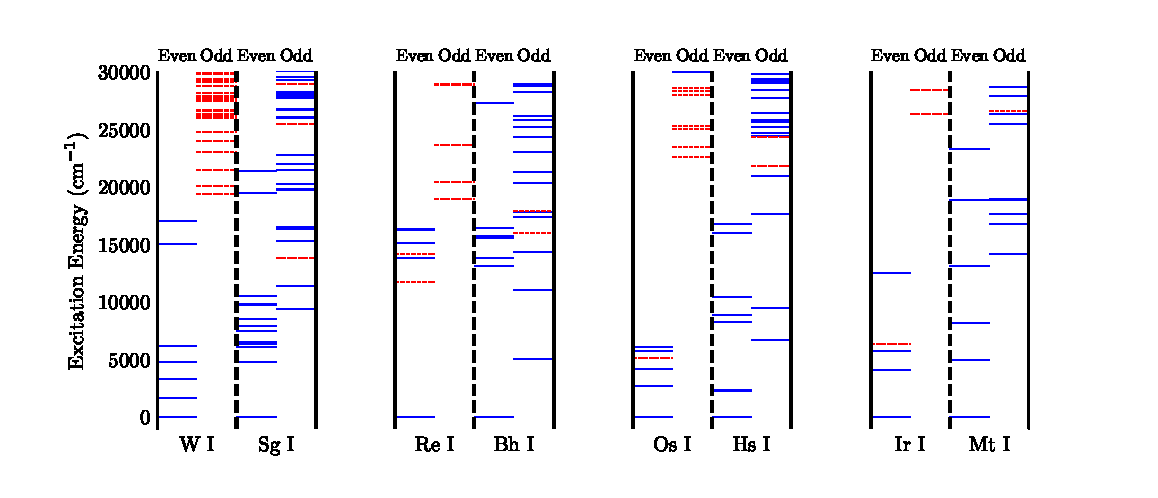
\includegraphics[scale=1]{./figures/Sg_Mt_Energy_Plot.eps} 
\caption{Comparison of low-energy excitations of SHE and their respective lighter analogs. For each element, the states are split between odd and even parities. The solid (blue) lines represent states with $6s^2$ or $7s^2$ in the electronic configuration for the lighter elements and SHE respectively. The dashed (red) lines are all other states where an $s$ electron has been excited from the filled $6s$ or $7s$ shell. Experimental energies were used for W \textsc{i}, Bh \textsc{i}, Hs \textsc{i} and Ir \textsc{i}. \cite{NIST_ASD}\label{fig:EL}}
\end{figure*}
\end{landscape}
Energy levels of SHE are calculated by solving the matrix eigenvalue problem (\ref{eq:CI}) separately for states of given value of the total angular momentum $J$ and parity. The specific details for each considered SHE are presented below. Most previous theoretical works on these SHE present the calculation of the first ionization potential, which we discuss in Section~\ref{sec:SHEIP}. Fig.~\ref{fig:EL} compares calculated spectra of low-lying states of SHE with experimental data on their lighter analogs. One can see a significant difference in the spectra of SHE and their lighter analogs, which is common for all considered atoms. Almost all low-lying odd states of lighter atoms correspond to the $6s-6p$ excitation from the ground state. In contrast to that, in SHE the $7s$ state is significantly lower on the energy scale than the $6d$ state due to relativistic effects. Therefore, dominant excitations occur from the $6d$ state, i.e. low-lying odd states correspond to the $6d-7p$ excitations from the ground state. Since the $6d-7p$ energy interval is smaller than the $6s-6p$ one, the density of odd states is higher for the SHE. 


\subsection{The Seaborgium Atom} \label{sec:Sg}


\begin{table*}[t] 
\caption{Low-energy spectrum of even- and odd-parity states in Bh \textsc{i}.   We present the energy and Land\'e $g$-factor for each state $J^{\text{parity}}$. We present $LS$- notations only for comparison with lighter analogs.  For SHE states where an analogous state cannot be found in the lighter analog the term is labeled according to the sequential number of the state ($n$) for the given $J^{\text{parity}}$ group, $n_{J}^{\text{parity}}$.\label{tab:SHESpectrumBh}}
 		\centering
 		\begin{tabular}{cl@{\hspace{0.5cm}}c@{\hspace{0.5cm}}r@{\hspace{0.5cm}}r} 
 		\toprule 
 \toprule 
&  \multicolumn{4}{c}{Bh \textsc{i}} \\
 \cmidrule{2-5}
&  \parbox{2cm}{Major \\ Configuration} & Term &   \parbox{1cm}{Energy \\ (cm$^{-1}$)}  &  \parbox{1.2cm}{Land\'{e} \\$g$-factor}  \\ 
 		\midrule 
\multicolumn{5}{c}{Even parity states}\\
 (1) &  $6d^5 7s^2$  &  $^6$S$_{5/2}$    & 0 & 1.78 \\ 
 (2) &   $6d^5 7s^2$  &  $^4$P$_{3/2}$    & 13 062 & 1.32 \\ 
 (3) &  $6d^5 7s^2$  &  $^4$G$_{7/2}$    &  13 828 & 1.15 \\ 
 (4) &   $6d^5 7s^2$  &  $^4$G$_{11/2}$    &  14 981 & 1.19 \\  
 (5) &   $6d^5 7s^2$  &  $^4$P$_{1/2}$   &  15 659 & 1.90 \\ 
 (6) &   $6d^5 7s^2$  &  $^4$G$_{9/2}$    & 16 447 & 1.17 \\  
\multicolumn{5}{c}{Odd parity states}\\
(7) &   $6d^4 7s^2 7p $  &  $^2$S$_{1/2}^{\rm_o}$    & 12 792 & 0.72 \\  
(8) &   $6d^4 7s^2 7p $   &  $^6$D$_{1/2}^{\rm_o}$   & 17 781 & 1.66 \\  
 (9) &   $6d^4 7s^2 7p $   &  $^6$D$_{3/2}^{\rm_o}$    & 19 483 & 1.09 \\  
(10) &   $6d^5 7s 7p$  &  $^8$P$_{5/2}^{\rm_o}$    & 22 228 & 2.08 \\  
(11) &   $6d^4 7s^2 7p $   &  $^6$P$_{3/2}^{\rm_o}$    & 22 533 & 1.74 \\  
(12) &   $6d^4 7s^2 7p $   &  $^6$D$_{5/2}^{\rm_o}$    & 22 930 & 1.26 \\  
 (13) &   $6d^5 7s 7p$  &  $^8$P$_{7/2}^{\rm_o}$    & 24 020 & 1.67 \\ 
(14)   &   $6d^4 7s^2 7p $   &  $^6$D$_{7/2}^{\rm_o}$    & 25 171 & 1.28 \\  
(15)  &   $6d^4 7s^2 7p $   &  $^6$D$_{9/2}^{\rm_o}$    & 26 587 & 1.21 \\  
 (16) &   $6d^4 7s^2 7p $  &  $^6$F$_{5/2}^{\rm_o}$    & 28 060 & 1.57 \\  
 (17) &  $6d^4 7s^2 7p $  & 3$_{1/2}^{\rm_o}$  & 29 823 & 0.44 \\ 
(18) &   $6d^4 7s^2 7p $ &  3$_{3/2}^{\rm_o}$  & 29 885 & 1.55 \\
(19) &  $6d^4 7s^2 7p $  & 3$_{7/2}^{\rm_o}$  & 31 078 & 1.24 \\ 
(20) &   $6d^4 7s^2 7p $ & 4$_{5/2}^{\rm_o}$  & 31 253 & 1.30 \\ 
(21) &   $6d^4 7s^2 7p $  & 4$_{7/2}^{\rm_o}$  & 32 814 & 1.37 \\ 
(22) &  $6d^4 7s^2 7p $  & 4$_{3/2}^{\rm_o}$  & 33 459 & 1.40 \\
(23) & $6d^4 7s^2 7p $  & 2$_{9/2}^{\rm_o}$  & 33 575 & 1.06 \\
(24) & $6d^4 7s^2 7p $  & 5$_{5/2}^{\rm_o}$     & 33 738 & 1.04 \\
(25) & $6d^4 7s^2 7p $  &  4$_{1/2}^{\rm_o}$  & 35 408 & 2.22 \\
(26) & $6d^4 7s^2 7p $  & 5$_{3/2}^{\rm_o}$   & 35 447 & 1.00 \\
(27) & $6d^4 7s^2 7p $  & 6$_{5/2}^{\rm_o}$  & 35 774 & 1.34 \\
(28) & $6d^4 7s^2 7p $  & 5$_{7/2}^{\rm_o}$   & 36 251 & 1.00 \\
(29) & $6d^4 7s^2 7p $  & 6$_{3/2}^{\rm_o}$    & 36 333 & 1.02 \\
(30) & $6d^4 7s^2 7p $  & 7$_{5/2}^{\rm_o}$    & 36 875 & 1.25 \\
(31) & $6d^4 7s^2 7p $  &  1$_{11/2}^{\rm_o}$    & 37 542 & 1.10 \\
(32) & $6d^4 7s^2 7p $  & 6$_{7/2}^{\rm_o}$  & 37 910 & 1.32 \\
(33)  & $6d^4 7s^2 7p $  & 7$_{3/2}^{\rm_o}$     & 37 954 & 1.05 \\
(34)  & $6d^5 7s 7p $  &  $^8$P$_{9/2}^{\rm_o}$    & 37 972 & 1.62 \\
(35) &  $6d^4 7s^2 7p $  & 4$_{9/2}^{\rm_o}$  & 38 336 & 1.23 \\  
(36) &  $6d^4 7s^2 7p $  & 8$_{5/2}^{\rm_o}$  & 39 454 & 1.19 \\
(37) &  $6d^4 7s^2 7p $  & 7$_{7/2}^{\rm_o}$  & 39 602 & 1.33 \\
(38) & $6d^4 7s^2 7p $  & 5$_{1/2}^{\rm_o}$  & 40 273 & 1.76 \\

  \bottomrule
 \bottomrule
 \end{tabular} 
 \end{table*} 
 \begin{table*}[t] 
\caption{Low-energy spectrum of even- and odd-parity states in Sg \textsc{i}.   We present the energy and Land\'e $g$-factor for each state $J^{\text{parity}}$. We present $LS$- notations only for comparison with lighter analogs.  For SHE states where an analogous state cannot be found in the lighter analog the term is labeled according to the sequential number of the state ($n$) for the given $J^{\text{parity}}$ group, $n_{J}^{\text{parity}}$.\label{tab:SHESpectrumSg}}
 		\centering 
 		\begin{tabular}{cl@{\hspace{0.5cm}}c@{\hspace{0.5cm}}r@{\hspace{0.5cm}}r@{\hspace{1cm}}l} 
 		\toprule 
 \toprule 
&  \multicolumn{4}{c}{Sg \textsc{i}} \\
 \cmidrule{2-5} 
& \parbox{2cm}{Major \\ Configuration} & Term  &   \parbox{1cm}{Energy \\ (cm$^{-1}$)}  &  \parbox{1.2cm}{Land\'{e} \\$g$-factor}  \\ 
 		\midrule 
\multicolumn{5}{c}{Even parity states}\\
 (1) &  $6d^4 7s^2$ &  $^5$D$_0$    & 0 & 0.00   \\ 
 (2) &  $6d^4 7s^2$ &  $^5$D$_1$     & 4 834 & 1.50   \\ 
 (3) &  $6d^4 7s^2$ &  $^5$D$_2$    & 7 614 & 1.44   \\ 
 (4) &  $6d^4 7s^2$ &  $^5$D$_3$   & 9 607 & 1.39  \\  
 (5) &   $6d^4 7s^2$ &  $^5$D$_4$    & 10 335 & 1.27 \\ 
 (6) &  $6d^4 7s^2$ &  $^5$2P$_0$    & 13 592 & 0.00  \\  
\multicolumn{5}{c}{Odd parity states}\\
(7) &  $6d^3 7s^2 7p$  & 1$_2^{\rm_o}$    & 14 717 & 0.57   \\  
(8) &   $6d^3 7s^2 7p$  &  1$_1^{\rm_o}$    & 17 043 & 0.71  \\  
 (9) &  $6d^3 7s^2 7p$  & 2$_2^{\rm_o}$    & 20 444 & 1.13  \\  
(10) &   $6d^3 7s^2 7p$  & 1$_3^{\rm_o}$    & 20 628 & 0.97   \\  
(11) &  $6d^4 7s 7p$  &  $^7$F$_0^{\rm_o}$   & 20 979 & 0.00  \\  
(12) &  $6d^3 7s^2 7p$  & 2$_1^{\rm_o}$     & 22 041 & 2.02   \\  
 (13) &  $6d^3 7s^2 7p$  &  1$_4^{\rm_o}$   & 24 132 & 1.11  \\ 
(14) &  $6d^3 7s^2 7p$  & 3$_1^{\rm_o}$    & 24 382 & 1.19  \\  
(15) &  $6d^4 7s 7p$  &  $^1$S$_0^{\rm_o}$   & 25 362 & 0.00 \\  
 (16) &  $6d^3 7s^2 7p$  & 2$_3^{\rm_o}$  & 25 966 & 1.29   \\  
 (17) &  $6d^3 7s^2 7p$  &  1$_{5}^{\rm_o}$   & 26 271 & 1.17  \\ 
(18) &   $6d^3 7s^2 7p$  & 3$_2^{\rm_o}$     & 26 420 & 1.22  \\
(19) &  $6d^4 7s 7p$  &  $^7$F$_1^{\rm_o}$  & 27 030 & 1.40  \\ 
(20) & $6d^3 7s^2 7p$  & 4$_2^{\rm_o}$   & 27 416 & 1.74  \\ 
(21) & $6d^4 7s  7p $  &  $^7$F$_2^{\rm_o}$   & 29 976 & 1.41   \\ 
(22) & $6d^3 7s^2 7p$  &  3$_0^{\rm_o}$ & 30 055 & 0.00 \\
(23) & $6d^3 7s^2 7p$  &  2$_4^{\rm_o}$ & 30 372 & 1.25 \\
(24) & $6d^3 7s^2 7p$ & 3$_3^{\rm_o}$  & 30 753 & 1.09 \\
(25) & $6d^3 7s^2 7p$  & 5$_1^{\rm_o}$  & 30 868 & 0.92 \\
(26) & $6d^3 7s^2 7p$ & 4$_3^{\rm_o}$ & 31 647 & 1.34  \\
(27) & $6d^3 7s^2 7p$  & 6$_2^{\rm_o}$  & 32 040 & 1.13 \\
(28) & $6d^3 7s^2 7p$  &  3$_4^{\rm_o}$ & 32 073 & 1.00  \\
(29) & $6d^3 7s^2 7p$ &  4$_0^{\rm_o}$ & 32 381 & 0.00 \\
(30) & $6d^3 7s^2 7p$ &  6$_1^{\rm_o}$  & 32 520 & 1.21  \\
(31) & $6d^4 7s  7p $  &  $^5$D$_3^{\rm_o}$ & 32 885 & 1.47  \\
(32) & $6d^3 7s^2 7p$  &  4$_4^{\rm_o}$ & 33 339 & 1.23  \\
(33) & $6d^3 7s^2 7p$  & 7$_2^{\rm_o}$  & 33 602 & 1.08 \\
(34) & $6d^3 7s^2 7p$  & 8$_2^{\rm_o}$  & 34 147 & 1.45 \\
(35) & $6d^3 7s^2 7p$  &  2$_{5}^{\rm_o}$ & 34 380 & 1.12  \\  
(36) & $6d^3 7s^2 7p$  & 6$_3^{\rm_o}$  & 34 538 & 1.13  \\
(37) & $6d^3 7s^2 7p$  & 7$_1^{\rm_o}$  & 35 110 & 1.42 \\
(38) & $6d^3 7s^2 7p$  & 7$_3^{\rm_o}$  & 35 897 & 1.31  \\
(39) & $6d^3 7s^2 7p$  &  5$_4^{\rm_o}$ & 36 629 & 1.29  \\
(40) & $6d^3 7s^2 7p$  & 9$_2^{\rm_o}$  & 36 695 & 1.24 \\
(41) & $6d^3 7s^2 7p$ & 8$_3^{\rm_o}$  & 36 846 & 1.18 \\
(42) & $6d^3 7s^2 7p$  & 8$_1^{\rm_o}$  & 37 169 & 1.30 \\
(43) & $6d^3 7s^2 7p$  &  6$_4^{\rm_o}$& 37 218 & 1.25 \\
(44) & $6d^3 7s^2 7p$  &  3$_{5}^{\rm_o}$ & 37 542 & 1.26 \\
(45) & $6d^3 7s^2 7p$  &  5$_0^{\rm_o}$  & 38 322 & 0.00 \\ 
(46) & $6d^3 7s^2 7p$  & 9$_3^{\rm_o}$  & 38 547 & 1.12 \\ 
(47) & $6d^3 7s^2 7p$  & 10$_2^{\rm_o}$  & 38 915 & 1.22 \\ 
(48) & $6d^3 7s^2 7p$  &  7$_4^{\rm_o}$ & 39 138 & 1.30 \\
(49) & $6d^3 7s^2 7p$  &  4$_{5}^{\rm_o}$ & 39 337 & 1.23 \\
(50) & $6d^3 7s^2 7p$  & 10$_3^{\rm_o}$  & 39 725 & 1.23 \\
(51) & $6d^3 7s^2 7p$  & 9$_1^{\rm_o}$  & 40 073 & 1.62 \\ 
  \bottomrule
 \bottomrule
 \end{tabular} 
 \end{table*} 
Seaborgium was first experimentally detected in 1974 \cite{Ghoirso1974}. Since the initial discovery there has been continued interest and study into its physical and chemical properties including the discovery of isotopes with longer lifetimes. There exist some experimental results for Sg \textsc{i} in the field of chemistry \cite{Schadel2012}. However, there are no spectroscopic results available.   The ground state configuration of Sg \textsc{i} is expected to be [Rn]$5f^{14}6d^47s^2$, similar to the ground state of its lighter homologue (W \textsc{i}, ground configuration:  [Xe]$4f^{14}5d^46s^2$). \\
\linebreak
We calculated the first 6 even parity states and the ground state was found  to be the [Rn]$5f^{14}6d^47s^2 \ ^5$D$_0$ state. To calculate the even states we use three reference configurations, $6d^47s^2$, $6d^5 7s$ and $6d^6$ to make states in the effective CI matrix (first terms in the expansion (\ref{eq:psi}) and in the CI effective Hamiltonian (\ref{eq:HCI})). All other states, which are treated as corrections to the states from reference configurations (second terms in the expansion (\ref{eq:psi}) and in the CI Hamiltonian (\ref{eq:HCI})) are obtained by exciting one or two electrons from the reference configurations.
Similarly, for odd parity states we use the reference states from the $6d^47s7p$, $6d^37s^27p$ and $6d^57p$ configurations.  All calculated even and odd energy levels are presented in Table \ref{tab:SHESpectrumSgBh}. Similar calculations were performed for W~\textsc{i}  using analogous reference states and the same parameters. Comparing these results to the experimental spectrum~\cite{NIST_ASD} we found a maximum discrepancy of $|\Delta| \approx 600 $~cm$^{-1}$ and expect a similar accuracy for our Sg~\textsc{i} calculations. Note that this accuracy is slightly better than what was reported in Ref.~\cite{DBHF2017} due to inclusion of a larger number of states into the effective CI matrix.

Comparing the spectrum of Sg~\textsc{i} in Table~\ref{tab:SHESpectrumSgBh} to the spectrum of W~\textsc{I}~\cite{NIST_ASD}, we can see the manifestation of relativistic effects. As discussed above, relativistic effects cause the $7s$ orbital in Sg \textsc{i} to be strongly contracted and more tightly bound in comparison to the $6s$ orbital in W~\textsc{I}. The same effects also push out the $6d$ orbital of Sg \textsc{i} in comparison to the $5d$ orbital in W \textsc{i}. In the  W~\textsc{i} spectrum there are low-lying states corresponding to the $6s \rightarrow 5d$ excitation from the ground state (e.g., the $5d^56s \ ^7$S$_3$ state at 2 951.29 cm$^{-1}$). In contrast, in the Sg~\textsc{i} spectrum, all low-lying even states belong to the  $6d^4 7s^2$ configuration. The relativistic effects are more apparent in the low-lying odd parity states of Sg~\textsc{i}. In W~\textsc{i} all odd states correspond to the $6s \rightarrow 6p$ excitation from the ground state, while in Sg~\textsc{i} most of the low-lying odd states correspond to the $6d \rightarrow 7p$ excitation.
Only a few of the Sg \textsc{i} predicted in the optical region correspond to the $7s \rightarrow 7p$ excitation. 

We calculate rates of electric dipole transitions from the ground state to excited states of the opposite parity using the approach described in Section~\ref{sec:Isoshift}. The results are presented in Table~\ref{tab:SHEE1transitionSgBh}. There are not many such transitions due to the zero value of the total angular momentum $J$ in the ground state. Because of that, the transitions are only allowed to the odd states with $J=1$. A few transitions are good candidates for the detection. The transition with the highest transition rate is $^5$D$_0 \rightarrow 9_1^{\rm_o}$ ($\omega = 40 \ 073 \text{ cm}^{-1}$).

We also present the isotopic shift parameters, $F$ and $a$ from equations (\ref{eq:isoa}) and (\ref{eq:isoF}), in Table~\ref{tab:SHEE1transitionSgBh} for each respective E1 transition. The two isotopes we use are $^{269}$Sg  and $^{290}$Sg ($R_{rms,\text{269}} = 5.8814$ fm and $R_{rms,\text{290}}  = 6.0145$ fm respectively),  where $^{290}$Sg is the theoretically  metastable ($N=184$) isotope of Sg. 

\subsection{The Bohrium Atom}  \label{sec:Bh}

 Bohrium was first discovered in 1981 \cite{Munzenberg1981}. No atomic spectra have been measured or calculated for any Bh isotopes or ions. When calculating the energy spectrum of Bh \textsc{i}, we use a similar approach as with Sg \textsc{i}.  For the low-lying even parity spectrum we use an effective CI matrix build from the states of the $6d^5 7s^2$, $6d^6 7s$ and $6d^7$ reference configurations. For the odd parity spectrum we use the states from the $6d^5 7s 7p$, $6d^4 7s^2 7p$ and $7d^6 7p$ reference configurations. The lowest six even parity states and low-lying odd parity states are presented in Table~\ref{tab:SHESpectrumSgBh}. For an estimate of accuracy we calculated the low-lying spectrum of Re~\textsc{i} (the lighter analogue of Bh) with similar parameters. Comparing the CIPT calculated spectrum to the experimental spectrum \cite{NIST_ASD}, the energy discrepancy (with respect to the ground state) was $\Delta \approx 900$~cm$^{-1}$ for the even parity states, while for the odd parity states $\Delta \approx 2000$~cm$^{-1}$.\\
\linebreak
 The calculated Bh~\textsc{i} ground state is $6d^5 7s^2 \ ^6$S$_{5/2}$.  As with Sg~\textsc{i},  we see the relativistic effect of the tightly bound $7s$ electron which results in the primary excitation of the $6d$ electron. Comparing the spectrum of Bh~\textsc{i} with that of Re~\textsc{I} in Fig. \ref{fig:EL} we see that there are several low-lying states in Re~\textsc{I} corresponding to $6s \rightarrow 5d$ excitations (the lowest is at $11 754.52$~cm$^{-1}$), while there are no similar low-lying states in Bh~\textsc{i}.  The density of low-energy odd-parity states is much larger in Bh~\textsc{i} than in Re~\textsc{i}. The Bh \textsc{i} low odd-parity states are completely dominated by the $6d \rightarrow 7p$ excitations in calculated spectrum and and there are no  $7s \rightarrow 7p$ excitations. 
 The odd-parity state comparison between Bh~\textsc{i} and Re~\textsc{I} is similar to that of Sg~\textsc{i} and W~\textsc{i} in Section \ref{sec:Sg}. In the spectrum of Re~\textsc{i}~\cite{NIST_ASD} there do exist states corresponding to  $5d \rightarrow 6p$ transitions from the ground state; however, they occur much higher in the spectrum compared to Bh~\textsc{i} where the $6d \rightarrow 7p$ excitations dominate. It should be noted that the number of low-lying odd-parity states is larger in Bh~\textsc{i} than in Re \textsc{i}. The lowest odd state of Bh \textsc{i} occurs at $12 792$~cm$^{-1}$, whereas in Re~\textsc{i} the lowest odd state is at $18 950$~cm$^{-1}$.\\
 \linebreak
 Bh \textsc{i} has a large number of allowed low-energy optical E1 transitions from the ground state, which are presented  in Table \ref{tab:SHEE1transitionSgBh}. The isotope shift parameters, $a$ and $F$, are calculated using formulas (\ref{eq:isoa}) and (\ref{eq:isoF}) after calculating the atomic spectra for the theoretically meta-stable isotope of $^{270}$Bh using the CIPT method. We use the values of RMS nuclear radii  $ R_{rms,\text{270}} =  5.8879$ fm for $^{291}$Bh and $R_{rms,\text{291}} = 6.0207$ fm  for $^{291}$Bh.
 
\subsection{The Hassium atom} \label{sec:Hs}

Hassnium ($Z=108$) was first synthesized in 1984~\cite{Munzenberg1984}. We present the low-lying levels and the first ionization energy of Hs~\textsc{i} in Table~\ref{tab:SHESpectrumHsMt}. For the low-lying even spectrum effective CI reference states belong to the $6d^5 7s^2$, $6d^6 7s$ and $6d^7$ configurations. For the odd spectrum we use reference states of the $6d^5 7s 7p$, $6d^4 7s^2 7p$ and $7d^6 7p$ configurations.  Note that the half-filled $6d$ sub-shell makes computational methods particularly expensive. However, using the CIPT method the computation becomes tractable.  

Once again it is interesting to compare the spectra of Hs~\textsc{i} with the analogue Os~\textsc{i} in the period above. In the even states of Os~\textsc{i} there are states corresponding to the $6s \rightarrow 5d$ excitations from the ground state. In the Hs~\textsc{i} spectrum all low-lying even states belong to the  $6d^5 7s^2$ configuration. No states with the $7s \rightarrow 6d$ excitation were found. The odd states are similar to those of Sg and Bh, with the primary excitation $6d \rightarrow 7p$ in Hs~\textsc{i} while there are no  $5d \rightarrow 6s$ excitations in low Os~\textsc{i} spectrum. The odd states of Hs~\textsc{i} also lie much lower than those in Os~\textsc{i}.  The lowest odd state of Hs~\textsc{i} is 13 949 cm$^{-1}$, while the first odd state of Os~\textsc{i} occurs at 22 615.69 cm$^{-1}$ \cite{NIST_ASD}. 

The allowed strong optical E1 transitions from the low-lying odd states to the ground state ($^5$D$_{4}$) are presented in Table~\ref{tab:SHEE1transitionSgBh}. As with Bh \textsc{i} there is a large number of strong optical transitions. The transition with the largest rate is 3$_5^{\rm o}$ $\rightarrow$ $^5$D$_{4}$ ($\omega =$~39~268~cm$^{-1}$). Other possibly detectable transitions include 5$_3^{\circ}$ $\rightarrow$ $^5$D$_{4}$ ($\omega =$~34~812~cm$^{-1}$) and 2$_5^{\circ}$ $\rightarrow$ $^5$D$_{4}$ ($\omega= $~34~739~cm$^{-1}$).

We also present the isotopic shift parameters for the Hs E1 optical transitions in Table~\ref{tab:SHEE1transitionSgBh}. These were calculated from the theoretical spectra (calculated with the CIPT method) with isotopes $^{270}$Hs and $^{292}$Hs with RMS nuclear radii $R_{rms,\text{270}} = 5.8879$ fm for $^{292}$Hs and $R_{rms,\text{292}} = 6.0207$ fm for $^{270}$Hs.

\subsection{The Meitnerium Atom} \label{sec:Mt}

		\begin{table*}[t] 
\caption{Low-lying spectrum of even and odd states parity for Hs \textsc{i} .   We present the energy and Land\'e g-factor for each state $J^{\text{parity}}$. We present $LS$- notations only for comparison with lighter analogs. For SHE states where an analogous state cannot be found in the lighter analog the term is labeled according to the sequential number of the state ($n$) for the given $J^{\text{parity}}$ group, $n_{J}^{\text{parity}}$.\label{tab:SHESpectrumHs}}
 		\centering 
 		\begin{tabular}{cl@{\hspace{0.5cm}}c@{\hspace{0.5cm}}r@{\hspace{0.5cm}}r@{\hspace{1cm}}l@{\hspace{0.5cm}}c@{\hspace{0.5cm}}r@{\hspace{0.5cm}}r} 
 		\toprule 
 \toprule  		
& \multicolumn{4}{c}{Hs \textsc{i}}  \\
 \cmidrule{2-5}  \\
& \parbox{2cm}{Major \\ Configuration} & Term &   \parbox{1cm}{Energy \\ (cm$^{-1}$)}  &  \parbox{1.2cm}{Land\'{e} \\g-factor}    \\ 
 		\midrule 
  		 	\multicolumn{5}{c}{Even parity states}\\
 (1) &  $6d^6 7s^2$  &  $^5$D$_{4}$   & 0 & 1.37   \\ 
 (2) & $6d^6 7s^2$  &  $^5$D$_2$   & 2 102 & 1.38   \\  
 (3) &  $6d^6 7s^2$  &  $^5$D$_{0}$ & 7 400 & 0.00   \\ 
 (4) &  $6d^6 7s^2$  &  $^5$D$_{3}$ & 8 270 & 1.43   \\ 
 (5) &   $6d^6 7s^2$  &  $^5$D$_1$   & 9 285 & 1.41   \\ 
 (6) &    $6d^6 7s^2$  &  $^3$H$_{5}$ & 15 816 & 1.11\\ 
\multicolumn{5}{c}{Odd parity states}\\
  (7) &   $6d^5 7s^2 7p$  & 1$_2^{\rm_o}$    & 13 093 & 1.98  \\  
  (8) &  $6d^5 7s^2 7p$  & 1$_3^{\rm_o}$     & 15 600 & 1.58  \\ 
 (9) &  $6d^5 7s^2 7p$  & 2$_2^{\rm_o}$  & 23 708 & 1.30  \\ 
 (10) &  $6d^5 7s^2 7p$  & 2$_3^{\rm_o}$     & 26 492 & 1.16  \\ 
(11) &   $6d^6 7s 7p$  &  $^7$D$_{4}^{\rm_o}$   & 27 394 & 1.58  \\  
(12) &   $6d^5 7s^2 7p$  &  1$_1^{\rm_o}$   & 29 444 & 1.17  \\  
(13) &    $6d^5 7s^2 7p$  &  3$_2^{\rm_o}$    & 29 794 & 1.34  \\ 
(14) &   $6d^6 7s 7p$  &  $^7$D$_5^{\rm_o}$    &30 863 & 1.37   \\  
(15) &  $6d^5 7s^2 7p$  & 3$_3^{\rm_o}$     & 30 908 & 1.32  \\ 
(16) &   $6d^5 7s^2 7p$  & 4$_2^{\rm_o}$    & 31 165 & 1.33 \\ 
(17) &   $6d^5 7s^2 7p$  & 2$_4^{\rm_o}$      & 31 295 & 1.40   \\  
(18) &  $6d^5 7s^2 7p$  & 1$_0^{\rm_o}$  & 31 552 & 0.00  \\ 
(19) &  $6d^5 7s^2 7p$ & 3$_4^{\rm_o}$     & 32 522 & 1.26  \\ 
(20) &  $6d^5 7s^2 7p$ & 5$_2^{\rm_o}$   & 33 694 & 1.44  \\ 
(21) &  $6d^5 7s^2 7p$ & 4$_3^{\rm_o}$     & 33 920 & 1.03 \\ 
(22) &  $6d^5 7s^2 7p$ & 2$_1^{\rm_o}$      & 34 076 & 1.52 \\ 
(23) &  $6d^5 7s^2 7p$  & 2$_5^{\rm_o}$     & 34 739 & 1.20 \\ 
(24) &  $6d^5 7s^2 7p$ & 5$_3^{\rm_o}$   & 34 812 & 1.41 \\
(25) &  $6d^5 7s^2 7p$ & 4$_4^{\rm_o}$   & 35 689 & 1.23 \\ 
(26) &  $6d^6 7s 7p$  &  $^7$D$_{3}^{\rm_o}$  & 35 705 & 1.56 \\ 
(27) &  $6d^5 7s^2 7p$  & 3$_1^{\rm_o}$   & 35 990 & 1.81 \\ 
(28) &  $6d^6 7s 7p$  &  $^7$D$_2^{\rm_o}$  & 37 036 & 1.40 \\ 
(29) &  $6d^6 7s 7p$  & $^7$P$_{3}^{\rm_o}$ & 37 237 & 1.33 \\ 
(30) &  $6d^5 7s^2 7p$ & 5$_4^{\rm_o}$   & 37 443 & 1.18 \\ 
(31) &  $6d^5 7s^2 7p$ & 7$_2^{\rm_o}$   & 38 519 & 1.34 \\
(32) &  $6d^6 7s 7p$  &  $^7$P$_{4}^{\rm_o}$ & 39 025 & 1.29 \\ 
(33) &  $6d^5 7s^2 7p$  & 3$_5^{\rm_o}$   & 39 268 & 1.27 \\
(34) &  $6d^6 7s 7p$  &  $^7$D$_1^{\rm_o}$  & 39 512 & 2.11 \\ 
(35) &  $6d^5 7s^2 7p$  & 8$_3^{\rm_o}$  & 39 652 & 1.38 \\ 
(36) &  $6d^5 7s^2 7p $  & 9$_3^{\rm_o}$    &  40 783  &  1.19 \\
  \bottomrule
 \bottomrule
 \end{tabular} 
 \end{table*} 
 
 		\begin{table*}[t] 
\caption{Low-lying spectrum of even and odd states parity for  Mt \textsc{i}.   We present the energy and Land\'e g-factor for each state $J^{\text{parity}}$. We present $LS$- notations only for comparison with lighter analogs. For SHE states where an analogous state cannot be found in the lighter analog the term is labeled according to the sequential number of the state ($n$) for the given $J^{\text{parity}}$ group, $n_{J}^{\text{parity}}$.\label{tab:SHESpectrumMt}}
 		\centering 
 		\begin{tabular}{cl@{\hspace{0.5cm}}c@{\hspace{0.5cm}}r@{\hspace{0.5cm}}r@{\hspace{1cm}}l@{\hspace{0.5cm}}c@{\hspace{0.5cm}}r@{\hspace{0.5cm}}r} 
 		\toprule 
 \toprule  		
&		\multicolumn{4}{c}{Mt \textsc{i}} \\
 \cmidrule{2-5} \cmidrule{6-9} \\
&  \parbox{2cm}{Major \\ Configuration} & Term &   \parbox{1cm}{Energy \\ (cm$^{-1}$)}  &  \parbox{1.2cm}{Land\'{e} \\g-factor}  \\ 
 		\midrule 
  		 	\multicolumn{5}{c}{Even parity states}\\
 (1) & $6d^7 7s^2$  &  $^4$F$_{9/2}$ & 0 & 1.265 \\ 
 (2) &  $6d^7 7s^2$  &  $^4$F$_{3/2}$  & 5 047 & 1.214 \\  
 (3) &   $6d^7 7s^2$  &  $^4$F$_{5/2}$ & 7 996 & 1.222 \\ 
 (4) &   $6d^7 7s^2$  &  $^4$F$_{7/2}$ & 12 628 & 1.213 \\ 
 (5) &   $6d^7 7s^2$  &  $^2$G$_{3/2}$ & 17 368 & 0.931 \\ 
 (6) & $6d^7 7s^2$  &  $^2$G$_{5/2}$   & 18 467 & 1.409\\ 
\multicolumn{5}{c}{Odd parity states}\\
  (7) &   $6d^6 7s^2 7p $  & 1$_{7/2}^{\rm_o}$   & 21 879 & 1.44 \\  
  (8) &   $6d^6 7s^2 7p $  &  1$_{9/2}^{\rm_o}$ & 24 388 & 1.33 \\ 
 (9) &   $6d^6 7s^2 7p $  & 1$_{3/2}^{\rm_o}$  & 24 524 & 1.51 \\ 
 (10) &   $6d^6 7s^2 7p $ & 1$_{5/2}^{\rm_o}$   & 25 990 & 1.25 \\ 
(11)  &   $6d^6 7s^2 7p $  & 2$_{5/2}^{\rm_o}$   & 31 975 & 1.54 \\  
(12) &  $6d^6 7s^2 7p $  &1$_{1/2}^{\rm_o}$    & 32 851 & 0.81 \\  
(13) &  $6d^7 7s  7p$  &  $^{6}$D$_{9/2}^{\rm_o}$ & 33 505 & 1.40 \\ 
(14) &  $6d^6 7s^2 7p $  & 2$_{1/2}^{\rm_o}$   & 34 665 & 1.51\\  
(15) &   $6d^6 7s^2 7p$  & 2$_{7/2}^{\rm_o}$    & 35 117 & 1.29 \\ 
(16) &   $6d^6 7s^2 7p$  & 2$_{3/2}^{\rm_o}$     & 36 159 & 1.13 \\ 
(17) &   $6d^7 7s 7p$  &  $^6$F$_{11/2}^{\rm_o}$   & 38 027 & 1.31 \\  
(18) &   $6d^6 7s^2 7p$& 3$_{7/2}^{\rm_o}$   & 38 450 & 1.17 \\ 
(19) & $6d^6 7s^2 7p$  & 3$_{9/2}^{\rm_o}$    & 39 296 & 1.13 \\ 
(20) & $6d^6 7s^2 7p$  & 2$_{11/2}^{\rm_o}$     & 41 310 & 1.33 \\ 
 \bottomrule
 \bottomrule
 \end{tabular} 
 \end{table*} 
Meitnerium ($Z=109$) was first synthesized in 1982 \cite{Munzenberg1982}. The ground state of Mt~\textsc{i} is expected to follow that of the element in the above period  (Ir) with [Rn]$5f^{14}6d^{7}7s^2 \ ^4$F$_{9/2}$ which we confirm in the calculated spectrum presented in Table \ref{tab:SHESpectrumHsMt}.\\

We use the same method as for previous elements to calculate the low-lying spectrum of Mt~\textsc{i}. We present the lowest six even states using the  $6d^7 7s^2$, $6d^8, 7s$ and $6d^9$ reference configurations. We also present the first 12 odd parity states for which the $6d^7 7s 7p$, $6d^6 7s^2 7p$ and $6d^8 7p$ configurations were used. The results are in Table~\ref{tab:SHESpectrumHsMt}. Comparison with lighter analog Ir~\textsc{i} shows similar trend as for other SHE Sg, Bh and Hs. 

 We also present the allowed E1 transitions for Mt and the respective isotope shift parameters in Table~ \ref{tab:SHEE1transitionSgBh}. The high energy of the odd states in Mt~\textsc{i} result in a small number of allowed E1 transitions within optical region from the ground state compared to Bh and Hs.  Promising transitions for future measurement include $^6$F$_{11/2}^{\circ} \rightarrow ^4$F$_{9/2}$ ($\omega =$~38~027~cm$^{-1}$) and $^{6}$D$_{9/2}^{\circ} \rightarrow ^4$F$_{9/2}$ ($\omega =$ 33~505~cm$^{-1}$). All other rates are two or more orders of magnitude smaller. For the synthesized and metastable isotopes we use the RMS nuclear radii values, $R_{rms,\text{276}} = 5.9265$ fm  and $R_{rms,\text{293}} = 6.0330$ fm.
 
  \begin{table*}[t] 
 \caption{Strong electric dipole transitions and isotopic shift parameters for Sg \textsc{i}. Only direct optical transitions to the ground state satisfying the E1 transition selection rules are shown. Here $D_{\text{E1}}$ is the transition amplitude in a.u., $A_{\text{E1}}$ is the transition rate, $a$, $F$, and $\tilde{F}$ are calculated isotopic shift parameters for the charge radius. The numbers in parentheses correspond to the numbered states in Table \ref{tab:SHESpectrumSg}. \label{tab:SHEE1transitionSg}}
\begin{tabular}{l@{\hspace{0.01cm}}c@{\hspace{0.5cm}}r@{\hspace{0.5cm}}r@{\hspace{0.5cm}}r@{\hspace{0.5cm}}r@{\hspace{0.5cm}}r}  % @{} adds extra padding to the columns 
\toprule
\toprule
& State &   \parbox{1cm}{$D_{\text{E1}}$ \\ (a.u)} & \parbox{1cm}{$A_{\text{E1}}$ \\ { \small $(\times 10^{6} \ \text{s}^{-1})$ }} & \parbox{1cm}{$a  $ \\ (cm$^{-1}$)} & \parbox{1cm}{$F $ \\ ($\frac{\text{cm}^{-1}}{\text{fm}^{2}}$)} &   \multicolumn{1}{c}{\parbox{1cm}{$\tilde{F} $ \\ (cm$^{-1}$) }} \\
\midrule
 		\multicolumn{7}{c}{Sg \textsc{i} (Ground state: $^5$D$_0$)}  \\
 		\\
(8) &  1$_1^{\rm_o}$        & 0.639 & 1.36 & 9.41& 2.04 & 11.9   \\ 
(12) & 2$_{1}^{\rm_o}$          & -0.160 & 0.192 & -2.95 & -0.639 & -3.73 \\ 
(14) & 3$_{1}^{\rm_o}$         & 1.17  & 13.4 & 4.90 & 1.06 & 6.18  \\ 
(19) & $^3$P$_1^{\rm_o}$      & -0.163 & 0.353 & -19.7 & -4.25 & -24.8  \\ 
(25) & 5$_{1}^{\rm_o}$   & 0.592 & 6.97 & 6.58 & 1.42 & 8.30  \\ 
(30) &  6$_{1}^{\rm_o}$     & -0.412 & 3.95 & 7.01 & 1.52 & 8.85  \\ 
(37) &  7$_{1}^{\rm_o}$ & -0.302 & 2.67&  1.66 & 0.36 & 2.10  \\
 (42) & 8$_{1}^{\rm_o}$   & 0.148& 0.761 & 3.55 & 0.768 & 4.48  \\
(51) & 9$_{1}^{\rm_o}$   & 0.524 & 11.9 & -4.77& -1.03& -6.01 \\
\bottomrule
\bottomrule
\end{tabular}

\end{table*}

  \begin{table*}[t] 
 \caption{Strong electric dipole transitions and isotopic shift parameters for Bh \textsc{i}. Only direct optical transitions to the ground state satisfying the E1 transition selection rules are shown. Here $D_{\text{E1}}$ is the transition amplitude in a.u., $A_{\text{E1}}$ is the transition rate, $a$, $F$, and $\tilde{F}$ are calculated isotopic shift parameters for the charge radius. The numbers in parentheses correspond to the numbered states in Table \ref{tab:SHESpectrumBh}. \label{tab:SHEE1transitionBh}}
\begin{tabular}{l@{\hspace{0.01cm}}c@{\hspace{0.5cm}}r@{\hspace{0.5cm}}r@{\hspace{0.5cm}}r@{\hspace{0.5cm}}r@{\hspace{0.5cm}}r}  % @{} adds extra padding to the columns 
\toprule
\toprule
& State &   \parbox{1cm}{$D_{\text{E1}}$ \\ (a.u)} & \parbox{1cm}{$A_{\text{E1}}$ \\ { \small $(\times 10^{6} \ \text{s}^{-1})$ }} & \parbox{1cm}{$a  $ \\ (cm$^{-1}$)} & \parbox{1cm}{$F $ \\ ($\frac{\text{cm}^{-1}}{\text{fm}^{2}}$)} &   \multicolumn{1}{c}{\parbox{1cm}{$\tilde{F} $ \\ (cm$^{-1}$) }}  \\
\midrule
 \multicolumn{7}{c}{Bh \textsc{i} (Ground State: $^6$S$_{5/2}$)} \\
 		\\
(9)  & $^6$D$_{3/2}^{\rm_o}$     & -0.172 & 0.107 & 18.1 & 3.74 & 22.8  \\ 
(10) & $^8$P$_{5/2}^{\rm_o}$     & -0.474 &  0.812 & 83.4 & 17.2 & 105 \\ 
(11) &  $^6$P$_{3/2}^{\rm_o}$     & -0.494 & 1.38 & -101 & -20.7 & -127 \\ 
(12) &  $^6$D$_{5/2}^{\rm_o}$     & -0.0391 & 0.00611 & -120 & -24.6 & -151 \\ 
(13)  & $^8$P$_{7/2}^{\rm_o}$     & 0.500 & 0.858 & 84.5 & 17.4 & 107 \\ 
(14)  & $^6$D$_{7/2}^{\rm_o}$     & 0.345 & 0.471 & -63.3 & -13.0 & -79.7 \\ 
(16) & $^6$F$_{5/2}^{\rm_o}$     & 1.51 & 16.6 & -160 & -33.0 & -202 \\
(18)  & 3$_{3/2}^{\rm_o}$  & 1.50 & 30.0 & -64.9 & -13.4 & -81.7 \\
(19) & 3$_{7/2}^{\rm_o}$   & 1.75 & 23.3 & 44.0 & 9.06& 55.4 \\
(20) & 4$_{5/2}^{\rm_o}$   &  -0.433 & 1.90 & -101 & -20.7 & -127  \\
(21) & 4$_{7/2}^{\rm_o}$   &  1.88 & 31.2 & -380 & -78.4 & -479 \\
(22) & 4$_{3/2}^{\rm_o}$  &   -0.998 & 18.6 & -41.3 & -8.51& -52 \\
(24) & 5$_{5/2}^{\rm_o}$  &   -0.101 & 0.131 & -105 & -21.6 & -132 \\
(26) & 5$_{3/2}^{\rm_o}$   &   0.438 & 4.27 & -135 & -27.9 & -170 \\
(27) & 6$_{5/2}^{\rm_o}$  &   -1.06 & 17.1 & -364 & -74.9 & -458 \\
(28) & 5$_{7/2}^{\rm_o}$  &  0.0665 & 0.0361 & -34.7 & -7.15 & -43.7 \\
(29) & 6$_{3/2}^{\rm_o}$    &  0.160 & 0.615 & -70.6 & -14.5 & -88.9 \\
(30) & 7$_{5/2}^{\rm_o}$    &  -0.539 & 4.86 & -335 & -69.0 & -422\\
(33) & 6$_{7/2}^{\rm_o}$   &   -0.674 & 6.18 & -129 & -26.6 & -163 \\
(34) & 7$_{3/2}^{\rm_o}$   &  0.387 & 4.09 & -513 & -106 & -647 \\
(37) & 8$_{5/2}^{\rm_o}$   &  0.232 & 1.10 & -561 & -116 & -707\\
(38) & 7$_{7/2}^{\rm_o}$  &  0.516 & 4.13 & -364 & -75.1 & -459 \\
\bottomrule
\bottomrule
\end{tabular}

\end{table*}
  \begin{table*}[t] 
 \caption{Strong electric dipole transitions and isotopic shift parameters for Hs~\textsc{i}. Only direct optical transitions to the ground state satisfying the E1 transition selection rules are shown. Here $D_{\text{E1}}$ is the transition amplitude in a.u., $A_{\text{E1}}$ is the transition rate, $a$, $F$, and $\tilde{F}$ are calculated isotopic shift parameters for the charge radius. The numbers in parentheses correspond to the numbered states in Table \ref{tab:SHESpectrumHs}. \label{tab:SHEE1transitionHs}}
\begin{tabular}{l@{\hspace{0.01cm}}c@{\hspace{0.5cm}}r@{\hspace{0.5cm}}r@{\hspace{0.5cm}}r@{\hspace{0.5cm}}r@{\hspace{0.5cm}}r}  % @{} adds extra padding to the columns 
\toprule
\toprule
& State &   \parbox{1cm}{$D_{\text{E1}}$ \\ (a.u)} & \parbox{1cm}{$A_{\text{E1}}$ \\ { \small $(\times 10^{6} \ \text{s}^{-1})$ }} & \parbox{1cm}{$a  $ \\ (cm$^{-1}$)} & \parbox{1cm}{$F $ \\ ($\frac{\text{cm}^{-1}}{\text{fm}^{2}}$)} &   \multicolumn{1}{c}{\parbox{1cm}{$\tilde{F} $ \\ (cm$^{-1}$) }}  \\
\midrule
 		\multicolumn{7}{c}{Hs \textsc{i} (Ground State: $^5$D$_{4}$)} \\
 		\\
(8)  & 1$_{3}^{\rm_o}$     & 0.501 &  0.276 & 22.7 & 4.45 & 28.9 \\
(10) & 2$_{3}^{\rm_o}$      & 0.224 & 0.269 & 22.9 & 4.49 & 28.8  \\
(11) & $^7$D$_{4}^{\rm_o}$    & -1.11 & 5.66 & -29.1 & -5.70 & -36.6   \\
(14) & $^7$D$_5^{\rm_o}$     & 0.999 &  5.41& -26.2 & -5.15  \\
(15) & 3$_{3}^{\rm_o}$     & 0.208 & 0.370 & 16.2 & 3.18 & 20.4   \\
(17) & 2$_{4}^{\rm_o}$      & 0.0934 & 0.0603 & 5.54 & 1.09 & 6.98   \\ 
(19) & 3$_{4}^{\rm_o}$      & 0.120 & 0.112 & 18.5 & 3.62 & 23.2   \\
(21) & 4$_{3}^{\rm_o}$      & -0.150 & 0.253 & 20.7 & 4.05 & 26.0  \\
(23) & 2$_{5}^{\rm_o}$      & -1.13 & 9.88 & 12.3 & 2.42 & 15.5   \\
 (24) & 5$_{3}^{\rm_o}$    & 1.70 & 35.5 & 12.3 & 2.41 & 15.5  \\
(25) & 4$_{4}^{\rm_o}$      & 0.798 & 6.52 & 7.84 & 1.54 & 9.87  \\ 
(26)  &  $^7$D$_{3}^{\rm_o}$   & -0.493 & 3.20 & -33.3 & -6.53 & -41.9  \\ 
(29) & $^7$P$_{3}^{\rm_o}$  & -0.511 & 3.91 & -15.8 & -3.11 & -19.9  \\ 
(30) &5$_{4}^{\rm_o}$     & -0.297 & 1.04 & 1.95 & 0.382 & 2.45  \\ 
(32) & $^7$P$_{4}^{\rm_o}$  & 0.425 &  2.41 & -9.56 & -1.87 & -12.0 \\ 
(33) &3$_{5}^{\rm_o}$     & 2.64 & 77.5 & 5.16 & 1.01 & 6.49   \\ 
(35) & 7$_{3}^{\rm_o}$    & 2.10 & 80.0 & -2.30 & -0.451 & -2.89  \\ 
\bottomrule
\bottomrule
\end{tabular}

\end{table*}
  \begin{table*}[t] 
 \caption{Strong electric dipole transitions and isotopic shift parameters for Mt~\textsc{i}. Only direct optical transitions to the ground state satisfying the E1 transition selection rules are shown. Here $D_{\text{E1}}$ is the transition amplitude in a.u., $A_{\text{E1}}$ is the transition rate, $a$, $F$, and $\tilde{F}$ are calculated isotopic shift parameters for the charge radius. The numbers in parentheses correspond to the numbered states in Table \ref{tab:SHESpectrumMt}. \label{tab:SHEE1transitionMt}}
\begin{tabular}{l@{\hspace{0.01cm}}c@{\hspace{0.5cm}}r@{\hspace{0.5cm}}r@{\hspace{0.5cm}}r@{\hspace{0.5cm}}r@{\hspace{0.5cm}}r}  % @{} adds extra padding to the columns 
\toprule
\toprule
& State &   \parbox{1cm}{$D_{\text{E1}}$ \\ (a.u)} & \parbox{1cm}{$A_{\text{E1}}$ \\ { \small $(\times 10^{6} \ \text{s}^{-1})$ }} & \parbox{1cm}{$a  $ \\ (cm$^{-1}$)} & \parbox{1cm}{$F $ \\ ($\frac{\text{cm}^{-1}}{\text{fm}^{2}}$)} &   \multicolumn{1}{c}{\parbox{1cm}{$\tilde{F} $ \\ (cm$^{-1}$) }}  \\
\midrule
\multicolumn{7}{c}{Mt \textsc{i} (Ground State: $^4$F$_{9/2}$)}\\
 		\\
 (7)	& 1$_{7/2}^{\rm_o}$	  & 0.0537 & 0.00765 & 27.5& 5.10 & 34.5 \\
   (8)	& 1$_{9/2}^{\rm_o}$	 & 0.432 & 0.550 & 27.6 & 5.13 & 34.7 \\
 (13)	&	$^{6}$D$_{9/2}^{\rm_o}$  & 1.27 & 12.3 & -51.7 & -9.60 & -64.9  \\
  (15) & 2$_{7/2}^{\rm_o}$	   & -0.294 & 0.946 & 33.3 & 6.18 & 41.8 \\
 (17)	&	$^6$F$_{11/2}^{\rm_o}$    & -1.89 & 33.3 & -47.9& -8.89& -60.1 \\
  (19) 	& 3$_{9/2}^{\rm_o}$	    & 0.0954 & 0.112 & 19.0 & 3.53 & 23.9  \\ 
 (20) 	& 2$_{11/2}^{\rm_o}$	    & 0.170 & 0.344 & 25.7 & 4.78 & 32.3  \\
\bottomrule
\bottomrule
\end{tabular}

\end{table*}


\section{Ionization potentials and comparison with other data.} \label{sec:SHEIP}

As well as calculating the spectrum of neutral Sg, Bh, Hs and Mt we also calculated their first ionization potentials (IPs). To calculate the IP for each atom we use the same single-electron basis set for a neutral atom and an ion. The ionization potential is found as a difference between ground state energies of the atom and its ion. The effective CI matrix was built from all states of the $6d^n 7s$, $6d^{n-1}7s^2$ and $6d^{n+1}$ reference configurations ($n=4-7$ for Sg through to Mt). States that were treated perturbatively were obtained by exciting one or two electrons from the reference configurations and generating all single-determinant states from these configurations. We start from calculating the IPs of lighter analogs of the SHE to compare them with experiment. The results are in Table~\ref{tab:IP}. We also include in the table the results of the multi-configuration Dirac-Fock (MCDF) calculation~\cite{MCDF-Sg,MCDF-BhHs}. We do this because similar MCDF calculations have been used for the SHE (see Tables~\ref{tab:EE} and \ref{tab:SHEIP}). The CIPT values of the IPs agree with experiment within few percent (error $<$1\% for Ta, W, and Re, and $\sim$ 3\% for Os and Ir). We expect similar accuracy for the first IPs of SHE analogs presented in Table \ref{tab:SHEIP}.  For comparison, the difference between MCDF values of IPs of W, Re and Os and experimental IPs is larger than 10\% (Table~\ref{tab:IP}).

%is used to calculate the ground state of each SHE ion. We present our calculations in Table \ref{tab:SHEIP} along with other theoretical calculations using multi-configurational Dirac-Fock (MCDF)~\cite{Turler2013} and  calculations using relativistic Hartree-Fock with semi-empirical correction for core polarisation~\cite{Dzuba2016}.\\

%\begin{table}[t]
\begin{table}[h]
\caption{Theoretical and experimental ionization potentials of open $5d$-shell elements.  The CIPT energies are the results of the present work. \label{tab:IP}}
\begin{tabular}{llcccc}
%\begin{tabular}{ll@{\hspace{0.75cm}}c@{\hspace{0.75cm}}c@{\hspace{0.5cm}}c@{\hspace{0.5cm}}c@{\hspace{0.5cm}}c}
\toprule
\toprule
           &                  & \multicolumn{3}{c}{IP (eV)} \\
Atom &  \parbox{1cm}{Ionic \\ State} & $J$ &  Expt.~\cite{NIST_ASD}   & CIPT  & MCDF \\
\midrule
Ta    & $5d^3 6s$  & 1   & 7.549    & 7.57  & \\
W     & $5d^4 6s$ & 1/2 & 7.864   & 7.90  &  6.97~\cite{MCDF-Sg}  \\
Re    & $5d^5 6s$ & 3   &  7.833  &  7.85  &  6.84~\cite{MCDF-BhHs} \\
Os    & $5d^6 6s$ & 9/2 & 8.438  &  8.69  &  7.45~\cite{MCDF-BhHs} \\
Ir      & $5d^7 6s$ & 5    & 8.967 &  9.27  & \\
\bottomrule
\bottomrule
\end{tabular}
\end{table}

Table~\ref{tab:EE} shows some resonance (corresponding to strong electric dipole transitions from the ground state) excitation energies for SHE and their lighter analogs calculated in the present work and by the MCDF method~\cite{MCDF-Sg,MCDF-BhHs}. The energies for lighter elements are compared to experiment. Our values are taken from Tables~\ref{tab:SHESpectrumSgBh} and \ref{tab:SHESpectrumHsMt}; for the MCDF energies we present all results which can be found in~\cite{MCDF-Sg,MCDF-BhHs}. There is  a significant difference in the excitation energies of SHE, while for lighter atoms the difference is not so large. There is a $\sim$ 10\% difference from experiment in both calculations. There are too little data on the MCDF calculations to come to any conclusion about the reasons for the differences. %We believe that our results for excitation energies of SHE are more accurate because there are more carefully verified 
\begin{table}[h]
\caption{Some excitation energies (cm$^{-1}$) in open $6d$-shell SHE and their lighter analogs. The CIPT energies are the results of the present work.   \label{tab:EE}}
\begin{tabular}{lllccc}
\toprule
\toprule
Atom &  \multicolumn{2}{c}{State} &  Expt.~\cite{NIST_ASD}   & CIPT  & MCDF~\cite{MCDF-Sg,MCDF-BhHs} \\
\midrule

W  & $5d^46s^2$ & $^5$D$_1$ & 1670 &1502 & 1162 \\
      &                      & $^5$D$_2$ & 3325 & 2664 & 2581 \\

Re    & $5d^5 6s6p$ &  $^8$P$^{\rm o}_{5/2}$   &  18950  &    & 14000  \\

Os    & $5d^6 6s6p$ &  $^7$D$^{\rm o}_{5}$  & 23463  &  26000  &  20500 \\

Sg  & $6d^47s^2$ & $^5$D$_1$ &         &4834 & 4186 \\
      &                      & $^5$D$_2$ &        & 7614 & 7211 \\

Bh    & $6d^5 7s7p$ &  $^8$P$^{\rm o}_{5/2}$   &    & 2220   & 15100  \\

Hs    & $6d^5 7s^27p$ &  $^5$S$^{\rm o}_{2}$  &   &  13100  &  5100 \\
        &                           &  $^5$D$^{\rm o}_{3}$  &   &  15600  &  8600 \\

\bottomrule
\bottomrule
\end{tabular}
\end{table}

Finally, Table~\ref{tab:SHEIP} shows IPs of SHE and their ions. We included the result of our previous work on Db~\cite{LDFDb2018} together with the relativistic Hartree-Fock (RHF) calculations which include semi empirical core-polarisation correction~\cite{Dzuba2016} and the MCDF results~\cite{MCDF-Sg,MCDF-BhHs}. There are two sets of MCDF results. One, in the column marked as MCDF, is what directly comes from the MCDF calculations. We also presented prediction of MCDF IPs corrected by extrapolation of the difference with experiment from lighter atoms (marked as ``Extrap.''). As one can see from Table~\ref{tab:IP} the MCDF method tends to underestimate IPs by about 10\%. Therefore, multiplying the calculated IPs by a factor $\sim$ 1.1 extrapolated from lighter elements leads to better prediction of the IPs for SHE. Indeed, the extrapolated values are in better agreement with our CIPT calculations. Note however that the extrapolation assumes similarities between involved elements. In fact, they are significantly different. Ionization of lighter elements goes via removal of the $s$ electron ($6s$ electron for W, Re and Os). In contrast, ionization of SHE goes via removal of the $6d$ electron. RHF calculations (see Ref.~\cite{Dzuba2016} and Table~\ref{tab:SHEIP}) used a different type of extrapolation. Instead of extrapolating a final number, a term in the Hamiltonian was extrapolated. A term, simulating the effect of core polarisation, was added to the RHF Hamiltonian in Ref. \cite{Dzuba2016}. Its strength was chosen to fit IPs of lighter atoms. Then the same term was used for SHE. 

Studying IPs of SHE with open $6d$-shell shows a significant difference in trends compared to their lighter analogs. These differences are convenient to discuss by looking at the diagram in Fig.~\ref{fig:IPPlot}. The diagram shows trends in IPs of SHE with open $6d$-shell from Db to Mt together with the trends for lighter atoms from Ta to Ir. IPs for doubly ionized ions of lighter elements are also shown because they do not have external $s$-electrons, and further ionization of these ions goes via removal of a $d$-electron similar to what takes place for SHE. 

First, we note that the change of IPs from Ta to Ir is smooth and almost monotonic, apart from a small local minimum at Re atom. It shows increasing of IP towards the fully filled $5d$ shell. The ionization occurs via removal of a $6s$ electron. The $6s$ orbital is not very sensitive to the details of energy structure of other shells, which explains the smooth behaviour of the IP trend. In contrast, ionization of the SHE occurs via removal of a $6d$ electron. Strong relativistic effects manifest themselves in the trend of the IP change. A local maximum of the IP occurs for Sg atom that has four $6d$ electrons in the fully occupied $6d_{3/2}^4$ subshell. Removing an electron from a closed shell is difficult, therefore there is a local maximum. The next atom, Bh, has one more $6d$ electron, which has to occupy the $6d_{5/2}$ state. Due to large relativistic effects in SHE, there is a large fine structure interval between the  $6d_{3/2}$ and $6d_{5/2}$ states and therefore a significantly smaller IP for Bh (see Fig.~\ref{fig:IPPlot} and Table~\ref{tab:SHEIP}). A similar effect is known for an open $p$ shell where it is more pronounced. E.g., the IP of Bi, which has three $6p$ electrons, is smaller than for Pb, which has two $6p$ electrons corresponding to the closed $6p_{1/2}^2$ subshell. The effect is much more pronounced for SHE with an open $7p$ shell~\cite{FF113-115}. The IP of Mc ($Z$=115), which has three $7p$ electrons, is about 1.5 times smaller than the IP of Fl ($Z$=114), which has two $7p$ electrons.

To see whether a similar effect can be found in lighter atoms, we studied IPs of doubly ionized ions with an open $d$-shell (from $3d$ to $5d$). The ions were chosen because they do not have external $s$-electrons, and further ionization goes via removal of a $d$-electron. The results are shown in Fig.~\ref{fig:IPPlot}. Most IP values are taken from the NIST database~\cite{NIST_ASD}. However, NIST data for ions from Ta~III to Ir~III have poor accuracy. Therefore, we recalculated the IPs using the CIPT method. IPs of these ions show a different trend compared to the SHE. The maximum binding energy and hence the maximum IP is for a half filled $d$-shell in agreement with the non-relativistic Hund rule, which states that the maximum energy corresponds to the maximum possible value of the total spin.  This holds even for the heaviest of the three groups of ions. Thus, the SHE elements with the open $6d$ shell represents the only known example of a strong manifestation of relativistic effects, making  the energy difference between the $6d_{3/2}$ and $6d_{5/2}$ states more important than Hund's rule.

A similar manifestation of relativistic effects can be found in the trends of further ionization of the SHE ions (see Table~\ref{tab:SHEIP}). In many cases (e.g., the Bh and Hs ions) ionization from the $6d$ shell stops as soon as the fully filled $6d_{3/2}^4$ subshell is reached. Further ionization occurs from the $7s$ subshell.

\begin{table}[h]
\caption{Ionization potentials of open $6d$-shell SHE, including ions.  The CIPT energies are the results of the present work. \label{tab:SHEIP}}
\begin{tabular}{llccccc}
%\begin{tabular}{ll@{\hspace{0.75cm}}c@{\hspace{0.75cm}}c@{\hspace{0.5cm}}c@{\hspace{0.5cm}}c@{\hspace{0.5cm}}c}
\toprule
\toprule
           &                  & \multicolumn{4}{c}{IP (eV)} \\
 \parbox{1cm}{Atom \\ or ion} &  \parbox{1cm}{Ground \\ State} & $J$ & CIPT  & RHF\footnotemark[1]  & \parbox{1cm}{MCDF \\ \cite{MCDF-Sg,MCDF-BhHs}} & \parbox{1cm}{Extrap. \\ \cite{MCDF-Sg,MCDF-BhHs}} \\
\midrule
Db~I   &  $6d^3 7s^2$ & 2    & 7.01 & 6.75 &  &  \\
&&&&&&\\
Sg~I    & $6d^4 7s^2$ & 0   & 8.22 &  7.70 & 7.03  & 7.85 \\
Sg~II   & $6d^3 7s^2$ & 3/2 & 18.0 &          & 15.85 &  17.06 \\
Sg~III  & $6d^2 7s^2$ &    2 & 24.8 &          & 24.61 &  25.74 \\
&&&&&&\\
Bh~I    & $6d^5 7s^2$ & 5/2 & 8.03 &  8.63  & 6.82  & 7.7 \\
Bh~II   & $6d^4 7s^2$ & 0    & 19.0 &           & 16.55  & 17.5 \\
Bh~III  & $6d^4 7s$    & 1/2 & 26.2 &            & 25.64  & 26.6 \\
Bh~IV  & $6d^4$        & 0    & 36.8 &            & 36.33  & 37.3 \\
&&&&&&\\
Hs~I    & $6d^6 7s^2$ & 4   & 8.52 &  9.52   & 6.69  & 7.6 \\
Hs~II   & $6d^5 7s^2$ & 5/2 & 19.7 &           & 16.62  & 18.2 \\
Hs~III  & $6d^4 7s^2$ & 3   & 27.7 &            & 27.12  & 29.3 \\
Hs~IV  & $6d^4 7s$    & 1/2 & 40.5 &           & 36.59  & 37.7 \\
Hs~V   & $6d^4 $        & 0    & 50.6 &           & 50.37  & 51.2 \\
&&&&&&\\
Mt~I    & $6d^7 7s^2$ & 9/2 & 9.86 & 10.4     &   & \\
Mt~II   & $6d^6 7s^2$ & 4 & 20.7 &             &   & \\
Mt~III  & $6d^5 7s^2$ & 5/2 & 28.4 &             &   & \\
Mt~IV  & $6d^5 7s$    & 3 & 43.3 &             &   & \\
Mt~V    & $6d^5$        & 5/2 & 50.3 &             &   & \\
\bottomrule
\bottomrule
\footnotetext[1]{Relativistic Hartree-Fock with semi-empirical core polarisation correction~\cite{Dzuba2016}}
\end{tabular}
\end{table}

\begin{figure}
\centering
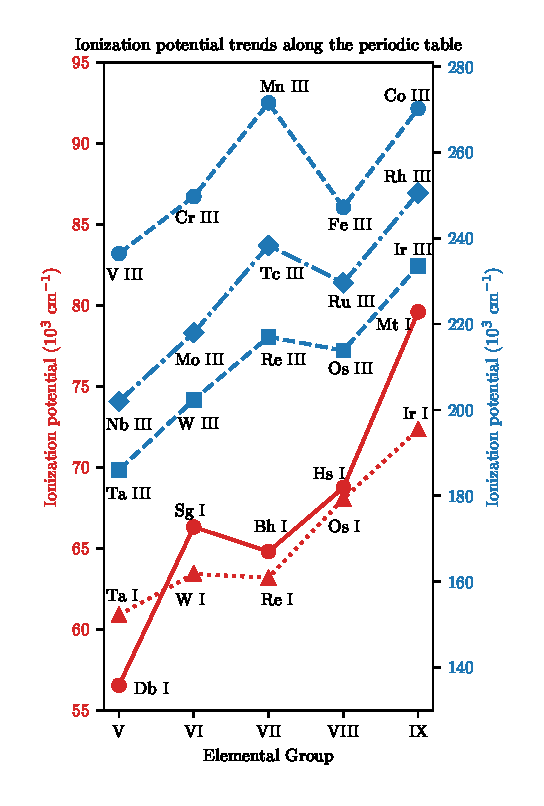
\includegraphics[scale=1.00]{./figures/Ionization_Plot.eps}
\caption{Plot of ionization trends for open $d$-shell elements. The IP trend lines for the doubly ionized elements (blue) use the scale on the right and the neutral IP trend lines (red) use the left. The IPs of neutral SHEs and the doubly ionized lighter homologues Ta~\textsc{iii}, W~\textsc{iii}, Re~\textsc{iii}, Os~\textsc{iii} and Ir~\textsc{iii} were calculated using the CIPT method. All other IPs are from Ref. \cite{NIST_ASD}. \label{fig:IPPlot}}
\end{figure}

\section{Conclusion}

Calculation of atomic spectra and optical E1 transitions for the elements in the superheavy region with open $d$-shells is novel. In spite of the extreme computational cost of existing methods, using perturbation theory we can calculate the low-lying energy states and relevant E1 transitions with a modest computational cost and with a small loss in accuracy \cite{DBHF2017}. In this work we presented the low-lying energy states for Sg \textsc{i}, Bh \textsc{i}, Hs \textsc{i} and Mt \textsc{i} including the optical transitions between the ground state and states of the opposite parity and their ionization potentials. For all SHEs we observed the relativistic effects, which contract the spectrum compared to their lighter analogs. This is advantageous as it results in a large number of states in the allowed E1 optical region and therefore enhances the likelihood of future measurements. These calculations will help to facilitate future experimental measurements of atomic spectra of these elements. We also presented the relevant isotopic field shift for optical E1 transitions for all four considered SHE. This may help the interpretation of future measurements and contribute to our understanding of the nuclear properties of elements in the superheavy region and potentially identify the existence of meta-stable superheavy isotopes in astronomical spectra.\\

 \chapter{Oganesson, $Z=118$}
The super heavy element (SHE) oganesson ($Z=118$) was first synthesized in 2006 at Dubna \cite{OganessianOg2006} and has recently been officially named and recognized \cite{Karol2016}.  It is also the first SHE and not naturally occuring element in the group of noble elements (Group 18) where the ground state has completely filled electron $np$ shells. Like other SHEs  ($Z>100$) it is of great experimental and theoretical interest due to the high relativistic nature  which may result in exotic and anomalous chemical and physical properties \cite{Pershina2009, Schwerdtfeger2014}. In general, experimental study of SHEs is difficult  due to the short lifetimes and low production rates. Og is no exception, where the only confirmed isotope ($^{294}$Og) has a halflife of 0.7 ms \cite{OganessianOg2006}. The study of Og and other SHEs is of great interest due to their exotic characteristics such as the large dependence on relativistic effects and the possible existence of long-lived isotopes of heavy nuclei in the ``island of stability''. \\
\linebreak
%Victor
The existence of long lived SHEs is predicted to occur when the ratio of neutrons to protons ($N/Z$) is large enough for the neutron-proton attraction to overcome  the Coulombic repulsion between protons (which scales as $Z^2$). Therefore the number of neutrons must increase faster than the number of protons requiring extremely neutron-rich isotopes to be  long-living\cite{OUL2004, HHO2013}.  Early nuclear shell models predict the nuclear shells stabilize for the ``magic'' numbers $Z=114$ and $N=184$\cite{OUL2004, HHO2013}. Synthesizing these neutron-rich isotopes is an extremely difficult challenge as the collision of two nuclei with a smaller $N/Z$ will always result in a neutron poor element.  However an alternate route to identify these long lived SHEs may be through analysing astrophysical data. Such avenues have already been explored with astrophysical data of  Przybylski's star suggesting that elements up to $Z=99$ have probably  been identified\cite{Polukhina2012, Gopka2008, Fivet2007}.  They may be decay products of long lived nuclei (see e.g.   \cite{DFW17} and references therein).  It is suspected that neutron rich isotopes may be created in cosmic events where rapid neutron capture (``$r$-process'') can occur due to large neutron fluxes during supernovae explosions, neutron star - (black hole and neutron star) mergers \cite{Goriely2011, Fuller2017, Friebel2018, Schuetrumpf2015}. To predict  atomic transition frequencies  for the neutron-reach isotopes the  calculated isotopic shifts should be added to the atomic transition frequencies measured in laboratories for the neutron-poor isotopes \cite{DFW17}. Search for these SHE in astrophysical data requires the strong electric dipole (E1) transitions which we calculate in this work.
 There has been a large amount of  theoretical work on the chemical and physical properties of Og with calculations of solid state and molecular properties \cite{Kullie2012, Shee2015, Nash1999, Nash2005, Peter2016}, electron affinities\cite{Pitzer1975, EliavOg1996, PershinaOg2008, Hangele2012, Goidenko2003}, and ionisation potentials and polarisabilities \cite{PershinaOg2008, Desclaux1973, Nash2005, Jerabek2018}. While some odd parity states and electric dipole (E1) transitions in the Og spectrum have been calculated in \cite{Indelicato2007} we present a more complete spectrum with both odd and even states to compare against similar states in the Rn spectrum. \\
There has been considerable work on both relativistic and quantum electrodynamic (QED) effects \cite{Pyykko1988, Jerabek2018, Goidenko2003, Eliav2015, Indelicato2007, Thierfelder2010} in Og. In this work we included both the Breit interaction and QED radiative effects. To aid in the experimental study of Og we use  theoretical methods to further study its physical properties. 
\section{CIPT calculation of } \label{sec:CIPT}
\begin{table*} [t!]
\centering
\caption{CIPT calculations of excitation spectrum, ionisation potential and electron affinity for Rn I with experimental results for comparison. Here $E_E$ and $E_T$ are experimental and theoretical CIPT excitation energies respectively with $\Delta = E_E - E_T$. We also present the calculated Land\'{e} $g$-factors and the energy difference between the experimental and theoretical excitation energies. (Originally published in \cite{LDFOg2018}) \label{tab:RnSpectrum}}
\begin{tabular}{l@{\hspace{0.5cm}}cc@{\hspace{0.5cm}}r@{\hspace{0.5cm}}r@{\hspace{0.5cm}}r@{\hspace{0.5cm}}r@{\hspace{0.5cm}}}
\toprule
\toprule
\multicolumn{7}{c}{Rn I}  \\
 & State & $J$ &  \multicolumn{1}{c}{\parbox{1cm}{$E_E$\cite{NIST_ASD} \\ (cm$^{-1}$)}}  &  \multicolumn{1}{c}{\parbox{1cm}{$E_T$ \\ (cm$^{-1}$)}} &  \multicolumn{1}{c}{$g_T$} &  \multicolumn{1}{c}{\parbox{1cm}{$\Delta$ \\ (cm$^{-1}$)}}  \\
 \hline
 \\
$6s^2 6p^6$      & $^1$S & 0 & 0    & 0    & 0    &        \\
$6s^2 6p^5 7s$ &    $^3$P$^{\rm_o}$         & 2  &  54 620  &  55 323     &  1.50     &  -703    \\
$6s^2 6p^5 7s$ &  $^1$P$^{\rm_o}$  & 1 &   55 989  & 56 607   &  1.18      &   -618    \\
$6s^2 6p^5 7p$ & $^3$S  &  1 &   66 245 & 67 171   & 1.76      &   -926     \\
$6s^2 6p^5 7p$ & $^3$D &  2 &   66 708 & 67 658  & 1.13     &   -950      \\
$6s^2 6p^5 6d$ & $^1$S$^{\rm_o}$ &   0 &  67 906  &   69 145  &  0          \\
$6s^2 6p^5 7p$ & $^3$D &  3 &   68 039  &  68 891  &  1.33      &   -852      \\
$6s^2 6p^5 7p$ & $^1$P & 1 &   68 332 &  69 313   & 1.09      & -981     \\
$6s^2 6p^5 7p$ & $^3$P &  2 &   68 790 &  69 749   & 1.37       &  -959    \\
$6s^2 6p^5 6d$ & $^3$P$^{\rm_o}$ &  1 &  68 891  & 70 002     &   1.36    & -1 111  \\
$6s^2 6p^5 7p$ & $^1$S &  0 &   69 744    &   70 800    &   0    &   -1 056      \\
$6s^2 6p^5 6d$ & $^3$F$^{\rm_o}$ &  4 &    69 798   &   70 742     &  1.25    &  -944   \\
$6s^2 6p^5 6d$ &  $^3$D$^{\rm_o}$ &  2     &   70 223   &  71 188 &   1.32    &   -965  \\
$6s^2 6p^5 6d$ & $^3$F$^{\rm_o}$ &  3 & 70 440  &  71 334 &  1.06     &    -894       \\
\multicolumn{7}{c}{Ionisation potential} \\
$6s^2 6p^5$ & $^2$P$^{\rm_o}$ & $3/2$ & 86 693 & 87 721 & 1.33 & -1 028   \\
\multicolumn{7}{c}{Electron Affinity} \\
$6s^2 6p^6 7s$ &   $^2$S & 1/2 &  & 1 868 & 2.00 &    \\
\bottomrule
\bottomrule
\end{tabular}

\end{table*}
\begin{table*} [t!]
\centering

\caption{CIPT calculations of excitation spectrum, ionisation potential and electron affinity for Og I. Here $E_T$ and $g_T$ are the theoretical CIPT excitation energies and Land\'{e} $g$-factors respectively.  (Originally published in \cite{LDFOg2018}) \label{tab:OgSpectrum}}
\begin{tabular}{@{\hspace{1cm}}r@{\hspace{1cm}}r@{\hspace{0.5cm}}l@{\hspace{1cm}}cc@{\hspace{1cm}}r@{\hspace{1cm}}r@{\hspace{1cm}}r}
\toprule
\toprule
\multicolumn{5}{c}{Og I} \\
 & State & $J$ & \multicolumn{1}{c}{\parbox{1cm}{$E_T$ \\ (cm$^{-1}$)}}  &  \multicolumn{1}{c}{$g_T$} & \parbox{1.5cm}{Ref. \cite{Indelicato2007}\\ (cm$^{-1}$)}  \\
 \hline
 \\
  $7s^2 7p^6$ & $^1$S & 0  &  0 & 0 & 0  \\
 $7s^2 7p^5 8s$  &  $^3$P$^{\rm_o}$  & 2 & 33 884 & 1.50 & 34 682 \\
 $7s^2 7p^5 8s$ & $^1$P$^{\rm_o}$ &  1   & 36 689    &  1.17  & 38 150   \\
 $7s^2 7p^5 8p$ & $^3$P &  1   & 49 186    &    1.60  &   \\
 $7s^2 7p^5 8p$ & $^3$D & 2    &  49 451   &   1.15    \\
 $7s^2 7p^5 8p$& $^3$D & 3    &  53 777   &    1.33 &    \\
 $7s^2 7p^5 8p$ & $^3$P &  1   & 53 881    &    1.24        \\
 $7s^2 7p^5 7d$ &  $^1$S$^{\rm_o}$ & 0    & 54 155    &  0  & 53 556    \\
$7s^2 7p^5 8p$ & $^3$P & 2     & 54 446 & 1.35 &  \\
$7s^2 7p^5 7d$ &  $^1$S$^{\rm_o}$ & 1    & 54 725    &  1.33 & 54 927 \\
$7s^2 7p^5 7d$ & $^3$F$^{\rm_o}$ & 4    &  54 938   &     1.25 & 48 474     \\
$7s^2 7p^5 7d$ & $^3$D$^{\rm_o}$ & 2    &  55 416    &    1.30 & 49 039 \\
$7s^2 7p^5 7d$ & $^3$F$^{\rm_o}$ &   3  &  55 622   &  1.06 & 49 603  \\
$7s^2 7p^5 8p$ & $^1$S & 0  &  55 729 & 0     \\
$7s^2 7p^5 7d$ & $^1$D$^{\rm_o}$ &  2   &  56 317   & 0.98 & 50 410  \\
$7s^2 7p^5 7d$ & $^5$F$^{\rm_o}$ &  3   & 56 343    &   1.25 & 50 168 \\
$7s^2 7p^5 7d$ & $^1$P$^{\rm_o}$ &  1   &  57 855   &   0.84  & 58 072  \\
\multicolumn{5}{c}{Ionisation potential} \\
$7s^2 7p^5$  & $^2$P$^{\rm_o}$ &   3/2  & 71 508    & 1.33  & 71 320\cite{Jerabek2018}    \\
\multicolumn{5}{c}{Electron Affinity} \\
 $7s^2 7p^6 8s$  & $^2$S  & 1/2    & -773$^{a}$    & 2.00  & -516 \cite{Goidenko2003}    \\


\bottomrule
\bottomrule
\end{tabular}

\begin{flushleft}
$^a$ Negative value indicates the state is bound.
\end{flushleft}
\end{table*}

In Table~\ref{tab:RnOgSpectrum} we present the results of our CIPT calculations for Rn I and Og I. We compare the Rn I CIPT calculations to the experimental results. The lack of experimental $g$-factors for Rn I make it difficult to confirm the correct identification of the states and therefore we must rely solely on the order of the energy levels. We find that there is good agreement between the experimental and theoretical states with an agreement with  $\Delta \approx -900$ cm$^{-1}$ with the largest discrepancy   $\Delta \approx -1239 $~cm$^{-1}$. We expect a similar accuracy for our Og I calculations (also presented in Table~\ref{tab:RnOgSpectrum}). \\

Comparing the spectrum of Rn  to Og we see that despite the similar electronic structure (with differing principal quantum numbers) there are significant differences. The Og spectrum is much more dense than Rn  with the first excitation lying more than 20~000~cm$^{-1}$ below the equivalent excitation in Rn. This results in an odd parity state which lies in the optical region. This makes the  state a good candidate for initial experimental measurement. In the final column of Table~\ref{tab:RnOgSpectrum} we present the states calculated in ref.~\cite{Indelicato2007}. This work also did not present $g$-factors which made comparing states uncertain, therefore we compared them by ordering energies. For 4 of the states there was good agreement with our results lying within $1000$ cm$^{-1}$ however for the other states there was a large discrepancy of $>4000$ cm$^{-1}$.  \\

Our calculated value of the ionisation potential of Og in Table~\ref{tab:RnOgSpectrum} is in excellent agreement with the value calculated in Ref.~\cite{Jerabek2018} ($E_{IP}=$71~320~cm$^{-1}$) where a CCSD(T) method was used.  

It has been shown that Og has a positive electron affinity which is an anomaly in the group of noble gases \cite{EliavOg1996, Goidenko2003, Eliav2015}. This is another consequence of the stabilized $8s$ orbital due to the large relativistic effects. Our calculation presented in Table \ref{tab:RnOgSpectrum}  confirms this with an electron affinity of 773 cm$^{-1}$ (0.095 eV) which is in good agreement with the coupled cluster value presented in \cite{Goidenko2003}. For comparison we also present the negative ion calculation for Rn I which is known to be unstable. All other negative ionic states of Og were found to be unstable.

\section{Electric dipole transitions of} \label{sec:E1}
 While Og  follows the expected trend for elements in noble group where each consecutive element has both a smaller IP and first excitation energy. However Og has some properties which can be considered exotic even amongst the Group 18 elements. According to the calculated spectrum in Table~\ref{tab:RnOgSpectrum} it is the only noble element which has an allowed optical electric dipole (E1) transition ($\omega < $40~000 cm$^{-1}$) from the ground state, unlike Rn where the first odd state lies at 57~334 cm$^{-1}$. \\
 
 The E1 transition amplitudes, $A_{\text{E1}}$, between states which satisfy the conditions of opposite parity and $\Delta J \leq 1$   are calculated using the many-electron wavefunctions created in the CIPT method and the self-consistent random-phase approximation which 
 %Victor 
includes polarization of  the atomic electron core by an external electromagnetic field. The details  of the method are presented  in Ref. \cite{Dzuba2018}. \\
 
The E1 transition rate is calculated using (in atomic units),
\begin{align} \label{eq:Transitionrate}
T_{E1} = \dfrac{4}{3}\left(\alpha \omega\right)^3\dfrac{ A_{\text{E1}}^2}{2J + 1}
\end{align}
where $J$ is the angular momentum of the upper state, $\alpha$ is the fine structure constant and $\omega$ is the frequency of the transition in atomic units. The transition amplitudes and transition rates for the allowed E1 transitions in Og are presented in Table~\ref{tab:E1_transitions}. In ref.~\cite{Indelicato2007} the major E1 transition rates were also calculated with a MCDF approach, these are included for comparison Table~\ref{tab:E1_transitions}. \\
\linebreak
We calculated the  rates of the $(n+1)s \rightarrow np$ transitions in lighter neutral noble elements Kr and Xe  and compared them to experimental values, these are presented in Table \ref{tab:E1_comp}. The experimental uncertainties are approximately $2\%$ for Xe I transitions \cite{Xe_BSD} and $~10$-$25\%$ for Kr I transitions\cite{Kr_BSD}. Comparing our calculated values to the experimental values in Table \ref{tab:E1_comp} we see the accuracy for these transitions is from 0.6\% to 17.7\%. We used the experimental energies to calculate the transitions rates of Kr I and Xe I using (\ref{eq:Transitionrate}) and since the uncertainty in the experimental energies are negligible the uncertainty in our calculations compared to experimental results in Table \ref{tab:E1_comp} is equivalent to the uncertainty in the square of the calculated transition amplitude $A_{E1}^2$. For our calculation of the Og I transition rates we needed to take into account the non-negligible uncertainty in the energies of our CIPT calculations.  Therefore assuming an accuracy of 18\% for $A_{E1}^2$ and an uncertainty of 3\% in the CIPT energy ($\left|\Delta\right| \approx 1000$~cm$^{-1}$) we expect a transition rate accuracy of 20\% for the $8s \rightarrow 7p$ optical transition ($\omega = 36~689$~cm$^{-1}$) of Og I in Table \ref{tab:E1_transitions}.  \\
\begin{table}[h]
\centering
\caption{Comparison of E1 transition rates between experimental and CIPT values for Kr I and Xe I. Here $A_{E1}$ is the transition amplitude in atomic units and $T_{E1}$ is the transition rate. \label{tab:E1_comp}}
\begin{tabular}{c@{\hspace{0.5cm}}c@{\hspace{1cm}}c@{\hspace{0.5cm}}c@{\hspace{0.5cm}}c}
\toprule
\toprule
State & $E_{\text{Exp}}$ & $A_{\text{E1}}$ & $T_{\text{E1, CIPT}}$ & $T_{\text{E1,Exp}}$  \\
&  (cm$^{-1}$) & (a.u.) &  ($\times 10^6$ s$^{-1}$) &  ($\times 10^6$ s$^{-1}$)  \\
\hline
\multicolumn{5}{c}{Kr I} \\
$^1$P$_1^{\rm_o}$ & 80 916 & 0.94  & 314  & 312\cite{Kr_BSD} \\
 $^3$P$_1^{\rm_o}$ & 85 846 & 0.87  & 320  & 316\cite{Kr_BSD}   \\
 \multicolumn{5}{c}{Xe I} \\
 $^1$P$_1^{\rm_o}$ & 68 045 & 1.18  & 295  & 273 \cite{Xe_BSD} \\
 $^3$P$_1^{\rm_o}$ & 77 185 & 0.98  & 298  & 253 \cite{Xe_BSD}  \\
\bottomrule
\bottomrule
\end{tabular}
\end{table}

\begin{table}[h]
\centering
\caption{Electric dipole transition amplitudes of Og I from the ground state $^1$S$_0$ to the excited states of odd parity and angular momenta $J=1$. Here $A_{E1}$ is the transition amplitude in atomic units and $T_{E1}$ is the transition rate. We include results of MCDF calculations from ref. \cite{Indelicato2007} for comparision. There is significant disagreement for the third transition however there is another transition in \cite{Indelicato2007} which has a rate ($986 \times 10^{6}$ s$^{-1}$) close to our calculated value. So, the disagreement  may be the result of a misprint in \cite{Indelicato2007}. (Originally published in \cite{LDFOg2018}).\label{tab:E1_transitions}}
\begin{tabular}{c@{\hspace{0.5cm}}c@{\hspace{1cm}}c@{\hspace{0.5cm}}c@{\hspace{0.5cm}}c}
\toprule
\toprule
State & $E_{\text{CIPT}}$ & $A_{\text{E1}}$ & $T_{\text{E1, CIPT}}$ & $T_{\text{E1,MCDF}}$ \cite{Indelicato2007}  \\
&  (cm$^{-1}$) & (a.u.) &  ($\times 10^6$ s$^{-1}$) &  ($\times 10^6$ s$^{-1}$)  \\
\hline
$^1$P$_1^{\rm_o}$ & 36 689 & 2.09 & 145 & 204\\
 $^1$S$_1^{\rm_o}$ & 54 725 & 0.727 & 58.4 & 55.3  \\
 $^1$P$_1^{\rm_o}$ & 57 855 & -2.67 & 936 & 9.9, 986* \\
\bottomrule
\bottomrule
\end{tabular}
\end{table}
Only the first transition in Table \ref{tab:E1_transitions} lies in the optical region and therefore it has the highest likelihood of being measured first. The large rate of the transition $^1$S$_0$~$\rightarrow$~$^1$P$_1^{\rm_o}$ is also promising for experimental measurement. 

\section{Electron density of } \label{sec:Relativistic}
The electron density of SHE gives insight into the effectiveness of the codes.



\begin{figure} 
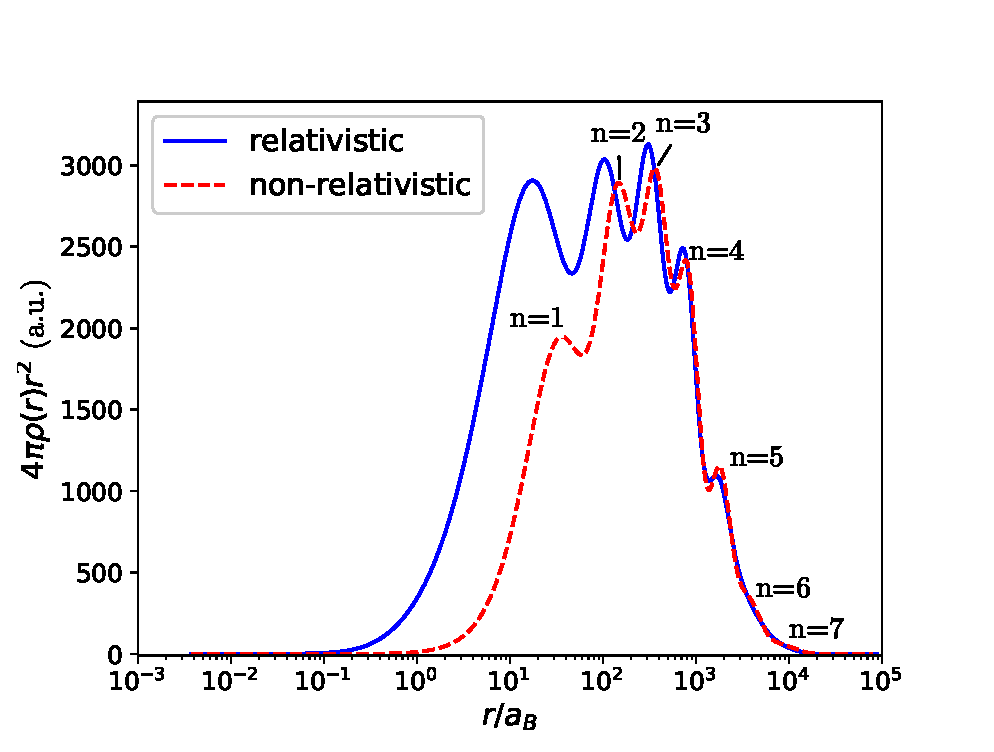
\includegraphics[scale=0.58]{./figures/Ogplot.eps}
\caption{Radial electron density, $4\pi\rho(r)r^2$ plot for Og I in both relativistic and non-relativistic approximations. The solid blue line and the dashed red line are non-relativistic and relativistic approximations respectively. The principle quantum peaks have been labeled for the non-relativic plot. (Originally published in \cite{LDFOg2018})\label{Og_plot}}
\end{figure}
\begin{figure}
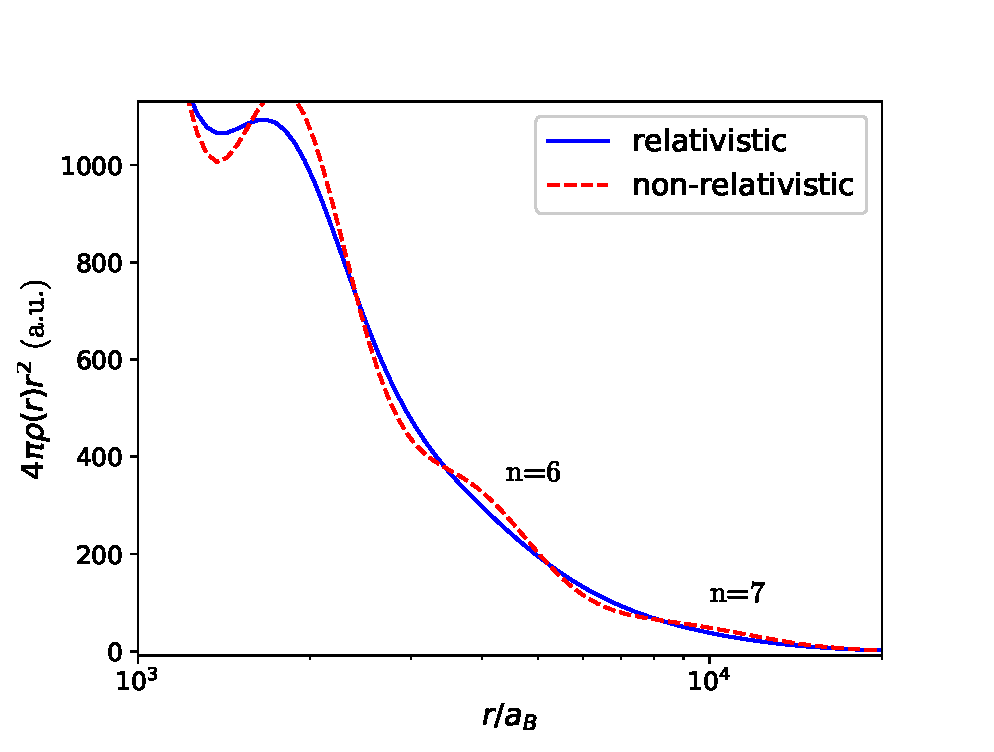
\includegraphics[scale=0.55]{./figures/Ogplot_zoom.eps}
\caption{Lower right section of  Figure~\ref{Og_plot}.\label{Og_plot_zoom}}
\end{figure}
It has been shown in Ref. \cite{Jerabek2018} using fermion localization that the electron density of Og is smoother than other group 18 analogues which have distinct atomic shells . The cause of this is the large relativistic effects in SHE which effectively smear out the shells into a smoother electron density (the same was shown for the nucleon density). The relativistic effects can also be seen by looking at the radial electron densities with relativistic and non-relativistic approximations. The Hartree-Fock radial electron density for Og is plotted on a logarithmic scale in Figure~\ref{Og_plot} in both the relativistic and non-relativistic approximations. There are a total of 7 peaks in the radial densities corresponding to the principle quantum numbers $n$ where lower shells have distinct peaks in both the relativistic and non-relativistic approximations. As expected, in the relativistic approximation the inner shells ($n=1,2,3$) shift closer to the nucleus however higher shells are relatively unaffected ($n \geq 4$). This results in a similar density profile for the electrons a large distance away from the nucleus. \\

In Figure~\ref{Og_plot_zoom} we plot the tail of the density function in Figure~\ref{Og_plot}. Here we see that, while spread out, the principle shell peaks still exist in the non-relativistic approximation. However in the relativistic approximation the density has been smoothed out to such a degree that there are no discernible peaks. This supports the results in ref.~\cite{Jerabek2018} where they calculated the electron shell structure of Og I and found that it disappears for external shells due to the high relativistic effects. This can be explained as the large spin-orbit splitting doubles the number of sub-shells which overlap making the overall distribution smooth.\\

\chapter{Conclusion}
We have calculated low lying energy levels, electric dipole transition amplitudes and isotope shift for superheavy element
dubnium. Similar CIPT calculations for its lighter analog Ta indicate that the uncertainty of the results for the energies of 
Db is unlikely to exceed 500~cm$^{-1}$. Db is the first SHE with open $6d$ shell which is studied with the recently
developed CIPT method. 

We thank Julian Berengut, Daniel Czapski and Amy Geddes for useful discussions.
This work was funded in part by the Australian Research Council.

In this work we calculated the spectrum and E1 transitions for Og I including the ionisation potential. We demonstrated the accuracy of the calculations by comparing similar calculations of Rn I to experimental data and expect an uncertainty of no more than $|\Delta| \approx 1000$~cm$^{-1}$. We found the spectrum of Og I is dense compared to other elements in  group 18 with significantly lower ionisation potential and excited states which follows the periodic trend. This compact spectrum introduces an allowed optical E1 transition which does not exist in other group 18 elements which presents a possibility for future experimental measurements. Our work also supports recent findings\cite{Jerabek2018} which suggest the electron shell structure of Og I is less prominent than lighter elements due to large relativistic effects which results in the outer electron density to becoming smooth. \\


\appendix



\chapter{Nilsson Orbitals}

\begin{figure}
\centering
\begin{subfigure}[b]{0.45\textwidth}
    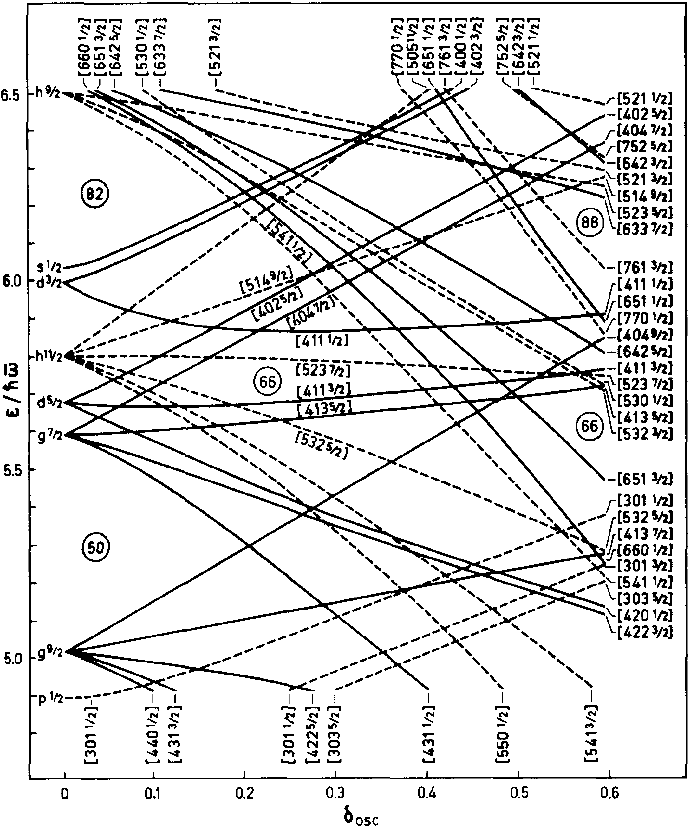
\includegraphics[width=\textwidth]{./figures/Nilsson/proton_deformed50.png}
    \caption{$50<Z<82$}
\end{subfigure}	
\quad
\begin{subfigure}[b]{0.45\textwidth}
    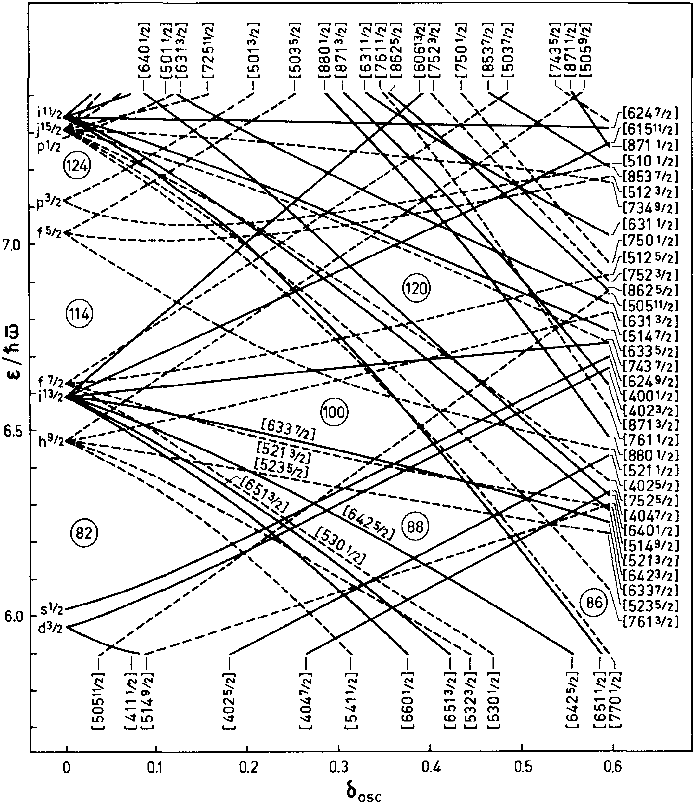
\includegraphics[width=\textwidth]{./figures/Nilsson/proton_deformed82.png}
    \caption{$Z>82$}
\end{subfigure}
\\
\begin{subfigure}[b]{0.48\textwidth}
    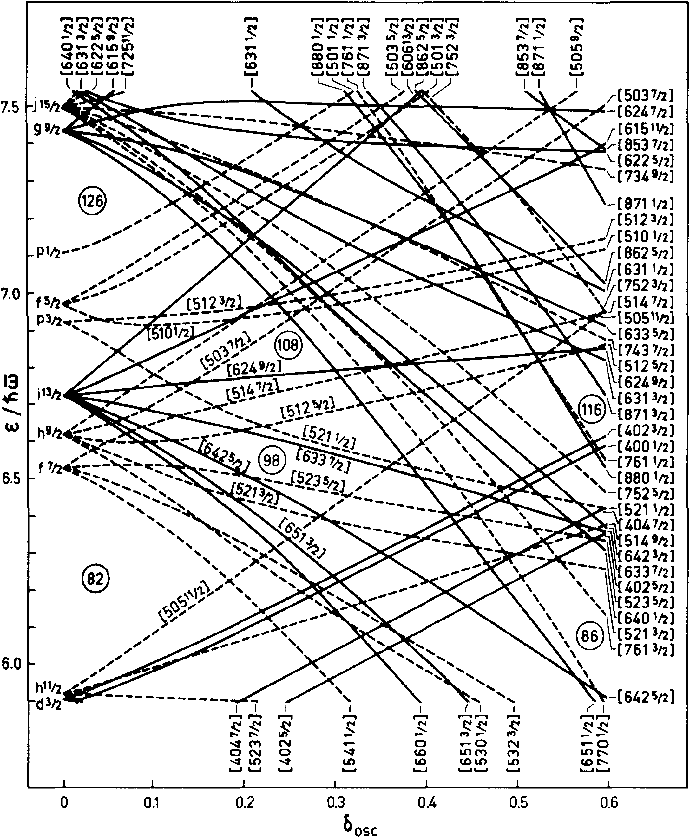
\includegraphics[width=\textwidth]{./figures/Nilsson/neutron_deformed82.png}
    \caption{$82<N<126$}
\end{subfigure}	
\quad
\begin{subfigure}[b]{0.48\textwidth}
    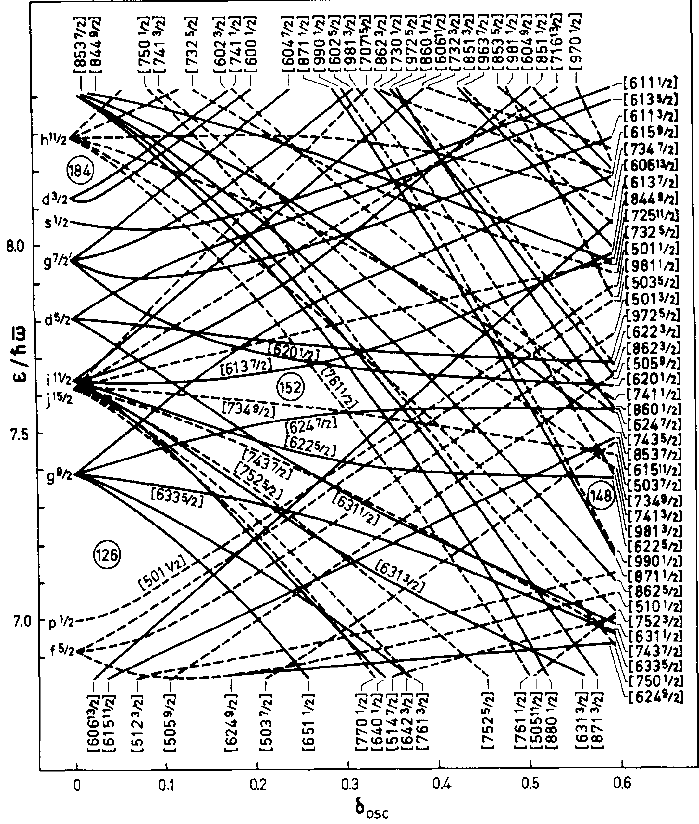
\includegraphics[width=\textwidth]{./figures/Nilsson/neutron_deformed126.png}
    \caption{$N>126$}
\end{subfigure}
\caption{Nilsson energy diagrams for both protons and neutrons for prolate deformed nuclei. Here $\delta$ is a degree of deformation. The numbers in circles represent the magic numbers in the spherical limit. These figures have been taken from \cite{BohrMottVol2}}

\end{figure}



\begin{table} 
\centering
\begin{tabular}{c|c}
\toprule
\toprule
Filled $N$ Shell & $\sum 2n_z + 1 = \sum N - n_z + 1$ \\ [2pt]
\midrule
0 & 2\\
1 & 10\\
2 & 28\\
3 & 60\\
4 & 110\\
5 & 182 \\
\bottomrule
\bottomrule
\end{tabular}
\caption{This shows $\sum 2n_z + 1$ and $\sum N - n_z + 1$  for each completely filled $N$ shell in the Nilsson model. \label{table:FullShellNz} %These numbers are the same for protons and neutrons.
}
\end{table}

\begin{table}[htbp]
\centering
\begin{tabular}{|c|c|c|c|c|c|}
\toprule
\toprule
$l_m$      & $\Omega[Nn_z\Lambda]$ & $2n_z + 1$ & $N - n_z + 1$ & $\Sigma\Lambda$ & $\Omega - \Lambda$ \\
\midrule
1$s_{1/2}$ & $1/2[000]$            & 1          & 1             & 0       &   1/2     \\
1$p_{3/2}$ & $1/2[110]$            & 3          & 1             & 0      &   1/2      \\
1$p_{3/2}$ & $3/2[101]$            & 1          & 2             & 1/2   &   1/2           \\
1$p_{1/2}$ & $1/2[101]$            & 1          & 2             & -1/2    &   -1/2       \\
\midrule
1$d_{5/2}$ & $1/2[220]$            & 5          & 1             & 0      & 1/2        \\
1$d_{5/2}$ & $3/2[211]$            & 3          & 2             & 1/2    & 1/2           \\
1$d_{5/2}$ & $5/2[202]$            & 1          & 3             & 1       & 1/2        \\
2$s_{1/2}$ & $1/2[211]$            & 3          & 2             & -1/2      & -1/2         \\
1$d_{3/2}$ & $1/2[200]$            & 1          & 3             & 0         & -1/2      \\
1$d_{3/2}$ & $3/2[202]$            & 1          & 3             & -1       & -1/2        \\
\midrule
1$f_{7/2}$ & $1/2[330]$            & 7          & 1             & 0        & 1/2       \\
1$f_{7/2}$ & $3/2[321]$            & 5          & 2             & 1/2      & 1/2         \\
1$f_{7/2}$ & $5/2[312]$            & 3          & 3             & 1          & 1/2     \\
1$f_{7/2}$ & $7/2[303]$            & 1          & 4             & 3/2       & 1/2        \\
2$p_{3/2}$ & $1/2[321]$            & 5          & 2             & -1/2      & -1/2         \\
2$p_{3/2}$ & $3/2[312]$            & 3          & 3             & -1       & -1/2        \\
1$f_{5/2}$ & $1/2[310]$            & 3          & 3             & 0         & 1/2      \\
1$f_{5/2}$ & $3/2[301]$            & 1          & 4             & 1/2      & 1/2         \\
1$f_{5/2}$ & $5/2[303]$            & 1          & 4             & -3/2      & -1/2         \\
2$p_{1/2}$ & $1/2[301]$            & 1          & 4             & -1/2      & -1/2         \\
\midrule
1$g_{9/2}$ & $1/2[440]$            & 9          & 1             & 0        & 1/2       \\
1$g_{9/2}$ & $3/2[431]$            & 7          & 2             & 1/2      & 1/2         \\
1$g_{9/2}$ & $5/2[422]$            & 5          & 3             & 1        & 1/2       \\
1$g_{9/2}$ & $7/2[413]$            & 3          & 4             & 3/2      & 1/2         \\
1$g_{9/2}$ & $9/2[404]$            & 1          & 5             & 2        & 1/2       \\
1$g_{7/2}$ & $1/2[431]$            & 7          & 2             & -1/2      & -1/2         \\
1$g_{7/2}$ & $3/2[422]$            & 5          & 3             & -1          & -1/2     \\
1$g_{7/2}$ & $5/2[413]$            & 3          & 4             & -3/2      & -1/2         \\ 
1$g_{7/2}$ & $7/2[404]$            & 1          & 5             & -2        & -1/2       \\
2$d_{5/2}$ & $1/2[420]$            & 5          & 3             & 0         & 1/2      \\
2$d_{5/2}$ & $3/2[411]$            & 3          & 4             & 1/2      & 1/2         \\
2$d_{5/2}$ & $5/2[402]$            & 1          & 5             & 1    & 1/2  \\
2$d_{3/2}$ & $1/2[411]$            & 3          & 4             & -1/2     & -1/2          \\
2$d_{3/2}$ & $3/2[402]$            & 1          & 5             & -1       & -1/2        \\
3$s_{1/2}$ & $1/2[400]$            & 1          & 5             & 1/2       & 1/2        \\
\bottomrule
\bottomrule
\end{tabular}
\end{table}
\begin{table}[htbp]
\centering
\begin{tabular}{|c|c|c|c|c|c|}
\toprule
\toprule
$l_m$      & $\Omega[Nn_z\Lambda]$ & $2n_z + 1$ & $N - n_z + 1$ & $\Sigma\Lambda$ & $\Sigma$ ( $\Omega - \Lambda$) \\
\midrule
1$h_{11/2}$ & $1/2[550]$            & 11         & 1             & 0      & 1/2         \\
1$h_{11/2}$ & $3/2[541]$            & 9          & 2             & 1/2      & 1/2         \\
1$h_{11/2}$ & $5/2[532]$            & 7          & 3             & 1       & 1/2        \\
1$h_{11/2}$ & $7/2[523]$            & 5          & 4             & 3/2      & 1/2        \\
1$h_{11/2}$ & $9/2[514]$            & 3          & 5             & 2        & 1/2       \\
1$h_{11/2}$ & $11/2[505]$           & 1          & 6             & 5/2      & 1/2         \\
1$h_{9/2}$ & $1/2[541]$             & 9          & 2             & -1/2      & -1/2         \\
1$h_{9/2}$ & $3/2[532]$             & 7          & 3             & -1     & -1/2          \\
1$h_{9/2}$ & $5/2[523]$             & 5          & 4             & -3/2      & -1/2         \\
1$h_{9/2}$ & $7/2[514]$             & 3          & 5             & -2        & -1/2       \\
1$h_{9/2}$ & $9/2[505]$             & 1          & 6             & -5/2      & -1/2         \\
2$f_{7/2}$ & $1/2[530]$             & 7          & 3             & 0        & 1/2       \\
2$f_{7/2}$ & $3/2[521]$             & 5          & 4             & 1/2      & 1/2         \\
2$f_{7/2}$ & $5/2[512]$             & 3          & 5             & 1        & 1/2       \\
2$f_{7/2}$ & $7/2[503]$             & 1          & 6             & 3/2       & 1/2        \\
3$p_{3/2}$ & $1/2[521]$             & 5          & 4             & -1/2     & -1/2          \\
3$p_{3/2}$ & $3/2[512]$             & 3          & 5             & -1       & -1/2        \\
2$f_{5/2}$ & $1/2[510]$             & 3          & 5             & 0      & 1/2         \\
2$f_{5/2}$ & $3/2[501]$             & 1          & 6             & 1/2       & 1/2        \\
2$f_{5/2}$ & $5/2[503]$             & 1          & 6             & -3/2       & -1/2        \\
3$p_{1/2}$ & $1/2[501]$             & 1          & 6             & -1/2       & -1/2        \\
\midrule
1$i_{13/2}$ & $1/2[660]$            & 13         & 1             & 0        & 1/2       \\
1$i_{13/2}$ & $3/2[651]$            & 11         & 2             & 1/2        & 1/2       \\
1$i_{13/2}$ & $5/2[642]$            & 9          & 3             & 2        & 1/2       \\
1$i_{13/2}$ & $7/2[633]$            & 7          & 4             & 3/2      & 1/2         \\
1$i_{13/2}$ & $9/2[624]$            & 5          & 5             & 2        & 1/2       \\
1$i_{13/2}$ & $11/2[615]$           & 3          & 6             & 5/2      & 1/2         \\
1$i_{13/2}$ & $13/2[606]$           & 1          & 7             & 3         & 1/2      \\
2$g_{9/2}$  & $1/2[651]$            & 11         & 2             & -1/2        & -1/2       \\
2$g_{9/2}$  & $3/2[642]$            & 9          & 3             & -1          & -1/2     \\
2$g_{9/2}$  & $5/2[633]$            & 7          & 4             & -3/2       & -1/2        \\
2$g_{9/2}$  & $7/2[624]$            & 5          & 5             & -2        & -1/2       \\
2$g_{9/2}$  & $9/2[615]$            & 3          & 6             & -5/2      & -1/2         \\
1$i_{11/2}$ & $1/2[640]$            & 9          & 3             & 0         & 1/2      \\
1$i_{11/2}$ & $3/2[631]$            & 7          & 4             & 1/2      & 1/2         \\
1$i_{11/2}$ & $5/2[622]$            & 5          & 5             & 1       & 1/2        \\
1$i_{11/2}$ & $7/2[613]$            & 3          & 6             & 3/2      & 1/2         \\
1$i_{11/2}$ & $9/2[604]$            & 1          & 7             & 2       & 1/2        \\
1$i_{11/2}$ & $11/2[606]$*           & 1          & 7             & -3       & -1/2        \\
\vdots      & \vdots                & \vdots     & \vdots        & \vdots           \\
\midrule
1$j_{15/2}$ & $1/2[770]$            & 15         & 1             & 0          & 1/2     \\
1$j_{15/2}$ & $3/2[761]$            & 13         & 2             & 1/2       & 1/2        \\
1$j_{15/2}$ & $5/2[752]$            & 11         & 3             & 1           & 1/2    \\
1$j_{15/2}$ & $7/2[743]$            & 9          & 4             & 3/2        & 1/2       \\
1$j_{15/2}$ & $9/2[734]$            & 7          & 5             & 2         & 1/2      \\
1$j_{15/2}$ & $11/2[725]$            & 5          & 6             & 5/2         & 1/2      \\
1$j_{15/2}$ & $13/2[716]$            & 3          & 7             & 3       & 1/2        \\
1$j_{15/2}$ & $15/2[707]$            & 1          & 8             & 7/2       & 1/2        \\
\vdots      & \vdots                & \vdots     & \vdots        & \vdots           \\
\bottomrule
\bottomrule
\end{tabular}
\end{table}
\newpage
\section{Filled and Unfilled shells of Nuclei}
Below is a table of the filled and unfilled $N$ shells of the deformed nuclei of interest. For Eu isotopes there are two applicable deformations, large or small. Due to the relative electric quadrupole moment of the two isotopes we assumed a large deformation for $^{153}$Eu and small deformation for $^{151}$Eu.
\begin{table}[htbp]
\begin{adjustwidth}{-3cm}{-3cm}
\centering
\begin{tabular}{|c|c|c|c|}
\toprule
\toprule
Nuclei     & Deformation ($\delta$) & Protons & Neutrons \\
\midrule
$^{9}$Be   &                        
    &  \pbox{20cm}{Filled Shells: N/A \\
    $1s_{1/2}$: $\pm 1/2$ \\
    $1p_{3/2}$: $\pm 1/2$}              
    &  \pbox{20cm}{Filled Shells: N/A \\
    $1s_{1/2}$: $\pm 1/2$ \\
    $1p_{3/2}$: $\pm 1/2, \textcolor{red}{3/2}$}\\
\midrule
$^{21}$Ne  &       
    &  \pbox{20cm}{Filled Shells: N/A \\
    $1s_{1/2}$: $\pm 1/2$ \\
    $1p_{3/2}$: $\pm 1/2$, $\pm 3/2$ \\
    $1p_{1/2}$: $\pm 1/2$ \\
    $1d_{5/2}$: $\pm 1/2$}              
    &  \pbox{20cm}{Filled Shells: N/A \\
    $1s_{1/2}$: $\pm 1/2$ \\
    $1p_{3/2}$: $\pm 1/2$, $\pm 3/2$ \\
    $1p_{1/2}$: $\pm 1/2$ \\
    $1d_{5/2}$: $\pm 1/2$ $\textcolor{red}{3/2}$}\\
\midrule
$^{27}$Al  &       
    &  \pbox{20cm}{Filled Shells: N/A \\
    $1s_{1/2}$: $\pm 1/2$ \\
    $1p_{3/2}$: $\pm 1/2$, $\pm 3/2$ \\
    $1p_{1/2}$: $\pm 1/2$ \\
    $1d_{5/2}$: $\pm 1/2$, $\pm 3/2$, $\textcolor{blue}{5/2}$}              
    &  \pbox{20cm}{Filled Shells: N/A \\
    $1s_{1/2}$: $\pm 1/2$ \\
    $1p_{3/2}$: $\pm 1/2$, $\pm 3/2$ \\
    $1p_{1/2}$: $\pm 1/2$ \\
    $1d_{5/2}$: $\pm 1/2$, $\pm 3/2$, $\pm 5/2$}\\
\midrule
$^{163}$Dy & $\approx 0.2$ 
    &  \pbox{20cm}{Filled Shells: N = 0, 1, 2, 3 \\
    $1g_{9/2}$: Full Shell \\
    $1g_{7/2}$: $\pm 1/2$, $\pm 3/2$, $\pm 5/2$ \\
    $2d_{5/2}$: $\pm 1/2$, $\pm 3/2$ \\
    $1h_{11/2}$:$\pm 1/2$, $\pm 3/2$, $\pm 5/2$}              
    &  \pbox{20cm}{Filled Shells: N = 0, 1, 2, 3, 4 \\
    $1h_{11/2}$: Full Shell \\
    $2f_{7/2}$: $\pm 1/2$, $\pm 3/2$, $\textcolor{red}{5/2}$ \\
    $1h_{9/2}$: $\pm 1/2$, $\pm 3/2$ \\
    $1i_{13/2}$: $\pm 1/2$, $\pm 3/2$} \\
\midrule
$^{173}$Yb & $\approx 0.3$
    &  \pbox{20cm}{Filled Shells: N = 0, 1, 2, 3 \\
    $1g_{9/2}$: Full Shell \\
    $1g_{7/2}$: $\pm 1/2$, $\pm 3/2$, $\pm 5/2$ \\
    $2d_{5/2}$: $\pm 1/2$, $\pm 3/2$ \\
    $1h_{11/2}$:$\pm 1/2$, $\pm 3/2$, $\pm 5/2$, $\pm 7/2$ \\
    $2d_{3/2}$: $\pm 1/2$}              
    &  \pbox{20cm}{Filled Shells: N = 0, 1, 2, 3, 4 \\
    $1h_{11/2}$: Full Shell \\
    $2f_{7/2}$: $\pm 1/2$, $\pm 3/2$, $\pm 5/2$ \\
    $1h_{9/2}$: $\pm 1/2$, $\pm 3/2$, $\textcolor{red}{5/2}$ \\
    $1i_{13/2}$:$\pm 1/2$, $\pm 3/2$, $\pm 5/2$, $\pm 7/2$ \\
    $3p_{3/2}$: $\pm 1/2$} \\
\midrule
$^{177}$Hf &
    &  \pbox{20cm}{Filled Shells: N = 0, 1, 2, 3 \\
    $1g_{9/2}$: Full Shell \\
    $1g_{7/2}$: Full Shell \\
    $2d_{5/2}$: $\pm 1/2$, $\pm 3/2$, $\pm 5/2$ \\
    $1h_{11/2}$:$\pm 1/2$, $\pm 3/2$, $\pm 5/2$, $\pm 7/2$}              
    &  \pbox{20cm}{Filled Shells: N = 0, 1, 2, 3, 4 \\
    $1h_{11/2}$: Full Shell \\
    $2f_{7/2}$: Full Shell \\
    $1h_{9/2}$: $\pm 1/2$, $\pm 3/2$, $\textcolor{red}{5/2}$ \\
    $1i_{13/2}$:$\pm 1/2$, $\pm 3/2$, $\pm 5/2$, $\pm 7/2$} \\
\midrule
$^{179}$Hf & $\approx 0.1$
    &  \pbox{20cm}{Filled Shells: N = 0, 1, 2, 3 \\
    $1g_{9/2}$: Full Shell \\
    $1g_{7/2}$: Full Shell \\
    $2d_{5/2}$: $\pm 1/2$, $\pm 3/2$, $\pm 5/2$ \\
    $1h_{11/2}$:$\pm 1/2$, $\pm 3/2$, $\pm 5/2$, $\pm 7/2$}          
    &  \pbox{20cm}{Filled Shells: N = 0, 1, 2, 3, 4 \\
    $1h_{11/2}$: Full Shell \\
    $2f_{7/2}$: Full Shell \\
    $1h_{9/2}$: $\pm 1/2$, $\pm 3/2$, $\pm 5/2$ \\
    $1i_{13/2}$:$\pm 1/2$, $\pm 3/2$, $\pm 5/2$, $\pm 7/2$, $\textcolor{red}{9/2}$} \\
\midrule
$^{181}$Ta & $\approx 0.3$
    &  \pbox{20cm}{Filled Shells: N = 0, 1, 2, 3 \\
    $1g_{9/2}$: Full Shell \\
    $1g_{7/2}$: $\pm 1/2$, $\pm 3/2$, $\pm 5/2$, $\textcolor{blue}{7/2}$ \\
    $2d_{5/2}$: $\pm 1/2$, $\pm 3/2$ \\
    $1h_{11/2}$:$\pm 1/2$, $\pm 3/2$, $\pm 5/2$, $\pm 7/2$ \\
    $2d_{3/2}$: $\pm 1/2$ \\
    $1h_{9/2}$: $\pm 1/2$}              
    &  \pbox{20cm}{Filled Shells: N = 0, 1, 2, 3, 4 \\
    $1h_{11/2}$: Full Shell \\
    $2f_{7/2}$: Full Shell \\
    $1h_{9/2}$: $\pm 1/2$, $\pm 3/2$, $\pm {5/2}$ \\
    $1i_{13/2}$:$\pm 1/2$, $\pm 3/2$, $\pm 5/2$, $\pm 7/2$ \\
    $1p_{3/2}$: $\pm 1/2$ \\
    $1g_{9/2}$: $\pm 1/2$} \\
\bottomrule
\bottomrule

\end{tabular}
\end{adjustwidth}
\end{table}
\begin{table}[htbp]
\centering
\begin{tabular}{c|c|c|c}
\toprule
\toprule
Nuclei     & Deformation ($\delta$) & Protons & Neutrons \\
\midrule
$^{201}$Hg & $\approx 0$
    &  \pbox{20cm}{Filled Shells: N = 0, 1, 2, 3 \\
    $1g_{9/2}$: Full Shell \\
    $1g_{7/2}$: Full Shell \\
    $2d_{5/2}$: Full Shell \\
    $1h_{11/2}$: Full Shell \\
    $2d_{3/2}$: Full Shell}              
    &  \pbox{20cm}{Filled Shells: N = 0, 1, 2, 3, 4 \\
    $1h_{11/2}$: Full Shell \\
    $2f_{7/2}$: Full Shell \\
    $1h_{9/2}$: Full Shell \\
    $1i_{13/2}$: Full Shell \\
    $1p_{3/2}$: Full Shell \\
    $1f_{5/2}$: $\pm 1/2$, \textcolor{red}{3/2}} \\
\midrule
$^{229}$Th & $\approx 0.21$
    &  \pbox{20cm}{Filled Shells: N = 0, 1, 2, 3, 4 \\
    $1h_{11/2}$: Full Shell \\
    $1h_{9/2}$: $\pm 1/2$, $\pm 3/2$ \\
    $1i_{13/2}$: $\pm 1/2$, $\pm 3/2$}              
    &  \pbox{20cm}{Filled Shells: N = 0, 1, 2, 3, 4, 5 \\
    $1i_{13/2}$: Full Shell \\
    $1g_{9/2}$: $\pm 1/2$, $\pm 3/2$, $\textcolor{red}{5/2}$ \\
    $1i_{11/2}$: $\pm 1/2$, $\pm 3/2$ \\
    $1j_{15/2}$: $\pm 1/2$, $\pm 3/2$} \\
\midrule
$^{151}$Eu & $\leq 0.05$
    &  \pbox{20cm}{Filled Shells: N = 0, 1, 2, 3 \\
    $1g_{9/2}$: Full Shell \\
    $1g_{7/2}$: Full Shell \\
    $2d_{5/2}$: $\pm 1/2$, $\pm 3/2$, $\textcolor{blue}{5/2}$ }          
    &  \pbox{20cm}{Filled Shells: N = 0, 1, 2, 3, 4 \\
    $1h_{11/2}$: Full Shell \\
    $2f_{7/2}$:$\pm 1/2$, $\pm 3/2$, $\pm 5/2$} \\
\midrule
$^{153}$Eu & $> 0.25$
    &  \pbox{20cm}{Filled Shells: N = 0, 1, 2, 3 \\
    $1g_{9/2}$: Full Shell \\
    $1g_{7/2}$: $\pm 1/2$, $\pm 3/2$, $\textcolor{blue}{5/2}$ \\
    $2d_{5/2}$: $\pm 1/2$ \\ 
    $1h_{11/2}$:$\pm 1/2$, $\pm 3/2$, $\pm 5/2$}          
    &  \pbox{20cm}{Filled Shells: N = 0, 1, 2, 3, 4 \\
    $1h_{11/2}$: Full Shell \\
    $2f_{7/2}$:$\pm 1/2$, $\pm 3/2$ \\
    $1h_{9/2}$: $\pm 1/2$ \\
    $1i_{13/2}$: $\pm 1/2$} \\
\midrule
$^{167}$Er & $\approx 0.3$          
    &  \pbox{20cm}{Filled Shells: N = 0, 1, 2, 3 \\
    $1g_{9/2}$: Full Shell \\
    $1g_{7/2}$: $\pm 1/2$, $\pm 3/2$, $\pm 5/2$\\
    $2d_{5/2}$: $\pm 1/2$, $\pm 3/2$ \\
    $1h_{11/2}$:$\pm 1/2$, $\pm 3/2$, $\pm 5/2$, $\pm 7/2$ }              
    &  \pbox{20cm}{Filled Shells: N = 0, 1, 2, 3, 4 \\
    $1h_{11/2}$: Full Shell \\
    $2f_{7/2}$: $\pm 1/2$, $\pm 3/2$, $\pm 5/2$ \\
    $1h_{9/2}$: $\pm 1/2$, $\pm 3/2$ \\
    $1i_{13/2}$:$\pm 1/2$, $\pm 3/2$, $\pm 5/2$, $\textcolor{red}{7/2}$} \\
\midrule
$^{133}$Cs & $< 0$                  &         & \\
$^{131}$Xe & $< 0$                  &         & \\
\bottomrule
\bottomrule
\end{tabular}
\end{table}

\listoffigures
\listoftables

\bibliography{Thesis}
\bibliographystyle{thesis}
\end{document}


